%\epigraphfontsize{\small\itshape}
%\setlength\epigraphwidth{8cm}
%\setlength\epigraphrule{0pt}
%\epigraphfontsize{\small\itshape}

%\epigraph{There are two possible outcomes: If the result confirms the hypothesis, then you've made a measurement. If the result is contrary to the hypothesis, then you've made a discovery.}{---\textup{ Enrico Fermi}}
%\epigraph{Everyone knows how useful it is to be useful. No one seems to know how useful it is to be useless.}{---\textup{  Chuang Tzu, The Useless Tree}}
\section{An Overview of the Reconstruction Algorithms in SNO+}
A particle interaction happens in the SNO+ detector can produce Cherenkov or scintillation photons. These photons propagate through the detector, and they can trigger PMTs when they reach the PSUP. As described in the last chapter, if there are enough PMTs triggered within a defined time window, an event is defined by the trigger system and for the event, the time and charge information measured by the hit PMTs are recorded.

By utilizing the recorded time and charge information, reconstruction algorithms attempt to calculate the physics quantities of an event, including its vertex (position and time), direction and energy. A few sets of reconstruction algorithms (called ``fitters'') have been implemented in the SNO+ RAT software or still being developed. These fitters are based on different methods and they can be coordinated and optimized for the different detector situations or physics phases.

According to the physics quantities, the SNO+ fitters can be generally classified as:
\begin{itemize}
	\item Vertex fitter. A vertex fitter reconstructs the event position and time by utilizing the positions and timing information of the hit PMTs. Currently, vertex fitters have been used to process the data and simulations for the water and partial-fill phases. They are also ready for the scintillator and tellurium-loading phases.
	
    On the other hand, some particular events, such as radioactive background events emitting $\gamma$s, can create multiple vertices which are correlated. A multi-site or multi-vertex fitter will be useful for tagging and removing these events during the $0\nu\beta\beta$ search. This kind of fitter is being developed.

	\item Direction fitter. A direction fitter reconstructs the event direction by using the directional information from the Cherenkov photons, which cause ring-like patterns formed by the hit PMT positions. The direction fitter has been used in the water phase analysis. For the scintillator and tellurium-loading phases, since the Cherenkov patterns will be submerged in the scintillation photons, it requires the other efforts for the direction reconstruction, which is being developed currently. 
	
	\item Energy fitter. An energy fitter translates the number of photons created from an event to the kinetic energy. The optical response of each PMT, including the PMT detection efficiency, transmission probability, attenuation, and etc. Similar to the vertex fitters, the energy fitters currently have been used in the water and partial-fill phases, and they are ready for the scintillator and tellurium-loading phases.

	\item Muon track fitter. This fitter is used to reconstruct the tracks of cosmic muons. It treats a muon track as a straight line and by dividing the SNO+ detector into several XY-slices along z, it reconstructs the intersection points for each slice by utilizing the positions and timing information of the hit PMTs\cite{muonTrackRecon}. It is currently being developed for the scintillator and tellurium-loading phases. It will help to tag and reduce the cosmogenic backgrounds, especially the $^{11}$C backgrounds induced by the muon spallation on the liquid scintillators\cite{sorensen2016temperature}.
\end{itemize}

For a fitter, its performance is first tested on the Monte Carlo simulations of specific physics processes. Then it is tested on both the simulations and real data of the calibration runs. Once the algorithm gives proper results which are approved by the collaboration, it is implemented into the SNO+ RAT software to process the SNO+ simulations and data files.

For a specific SNO+ physics phase, the fitters for reconstructing different physics quantities of an event are integrated. Currently, there are three integrated fitters: the \texttt{Water Fitter} for the water phase, the \texttt{Partial Fitter} for the partial-fill phase, and the \texttt{Scint Fitter} for the scintillator phase and the tellurium loading phase. The fitter parameters, such as the optical parameters, fitter iterations, are coordinated and optimized based on simulations and calibration data from that specific physics phase. In addition, PMT selectors and classifiers are also included in the integrated fitters. The PMT selectors are used to remove the outliers of the hit PMTs for a specific fitter, such as the hit PMT probably triggered by the noises. These selectors can help to make the fitter more accurate or to boost up the fitter speed. The classifiers mainly use the reconstructed results to calculate specific quantities which describe the probability of determining an event as an expected signal or background.

In this chapter, a Multi-path (MP) reconstruction framework and its principles are discussed. It was developed by the University of Alberta group as an additional fitter to provide event vertex and direction reconstructions. In this framework, the fitters are able to be adapted for all the SNO+ physics phases by switching light path calculations as well as the input optical parameters, that is the reason why it is called "multiple paths". It was applied in the water phase to provide alternative information of the event position and direction; it also works as the vertex reconstruction algorithm for the \texttt{Partial Fitter}. After re-coordination for the scintillator phase and tellurium loading phase, I also show the potentials of the vertex fitter being applied in these two future phases.

In addition, potentials of extracting the directional information from the scintillator phase is also discussed in this chapter.

\section{Multi-path Position and Direction Reconstructions for the Water Phase}\label{sect:mpw}
In the SNO+ water phase, both of the cavity and the AV were filled with ultra-pure water. This is a relatively simple geometry since everything inside the PSUP sphere can be simplified as water if omitting the AV shell. Therefore, to explain the reconstruction concepts, I will start with the \texttt{MP water fitter} (the \texttt{MPW fitter}).

The \texttt{MPW fitter} fits for the vertex and direction of a triggered event in SNO+ water phase. It first fits for the event vertex, and then takes the results of the reconstructed position to fit for the event direction.

\subsection{Vertex Reconstruction}

To fit for the vertex with 4 parameters: $x,y,z$ and $t$, first the fitter creates a random position inside a sphere with a radius of $10~m$ (larger than the actual PSUP radius $r_{PSUP}=8.39~m$). Meanwhile, a random event time is also generated from a uniform distribution in the range of $[100,300~ns]$. The Class Library for High Energy Physics (\texttt{CLHEP}) is used for creating pseudo-random numbers. The random position and the random time are combined to form a random event vertex as the trial event vertex $\vec{X}_0$. See the Sect.~\ref{appendix:random_gen} for details.

For a triggered event, photons are created around the event position and propagate to the hit PMTs. In a simplified detector geometry model which neglects the effects from scattering, reflection and refraction, these photons are considered as propagating along straight lines connecting the trial event vertex to the hit PMTs. Then the fitter evaluates a timing parameter, called the time residual ($t_{res}$), which is defined as:
\begin{equation}
\label{tres_define}
t_{res}=t_{PMT} - t_{transit} - t_{event},
\end{equation}

where $t_{PMT}$ is the PMT trigger time recorded by the detector, $t_{event}$ is the time when an event occurs (event time), and $t_{transit}$ is the total transit time (or time of flight, $TOF$) taken by a photon traveling from the event position ($\vec{X}_{event}$) to the hit PMT ($\vec{X}_{PMT}$) and crossing different materials in the detector.

To calculate the $t_{transit}$, the fitter uses Cherenkov photons in a prompt time window (called ``prompt light''), set as $-10<t_{res}<10~ns$ for the \texttt{MPW fitter} and the photons are assumed to propagate in straight lines (straight light paths). By assuming straight light paths, complicated situations of the photon propagation are neglected, including the refraction and reflection when the lights cross boundaries between different detector materials, absorption and scattering from the materials, as well as the lensing effects caused by the spherical structure of the acrylic vessel. In this case, the $TOF$ can be simply calculated as $t_{transit}=|\vec{X}_{event}-\vec{X}_{PMT}|/v_{water}$, where $v_{water}$ is an average photon group velocity and it is an effective value obtained by tuning on the Monte Carlo simulations. Section \ref{sect:tuneGroupVelocity} will show the details about the tuning. Based on the reconstruction experiences from the SNO experiment, it was found that without these details, the fitter can still produce decent results that are consistent with the case using detailed calculations\cite{boulay2004direct,jones2011background}. Fig.~\ref{mpwdiagram_position} shows the straight light paths from the event position to the hit PMT positions.
\begin{figure}[htbp]
	\centering
   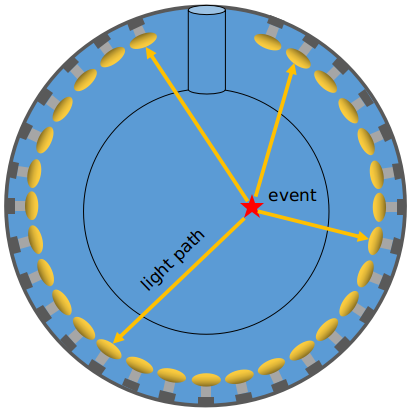
\includegraphics[width=6cm]{mpwDiagram.png}
	\caption{A diagram of straight light path for event position reconstruction in the SNO+ water phase geometry.}
	\label{mpwdiagram_position}
\end{figure}

An one-dimensional (1D) probability density function ($PDF$) is used for fitting the timing model, as shown in Fig.~\ref{fig:MPW_timingPDF}. This $PDF$ serves as a model of the timing responses of the triggered PMTs to an event to be fit. It was taken from the bench-top measurement of the individual PMT timing profile from SNO\cite{jillings1996photomultiplier} and was further tuned according to the measured $in-situ$ SNO+ detector responses to the calibration sources\cite{anderson2021optical}.

\begin{figure}[!htb]
	\centering
	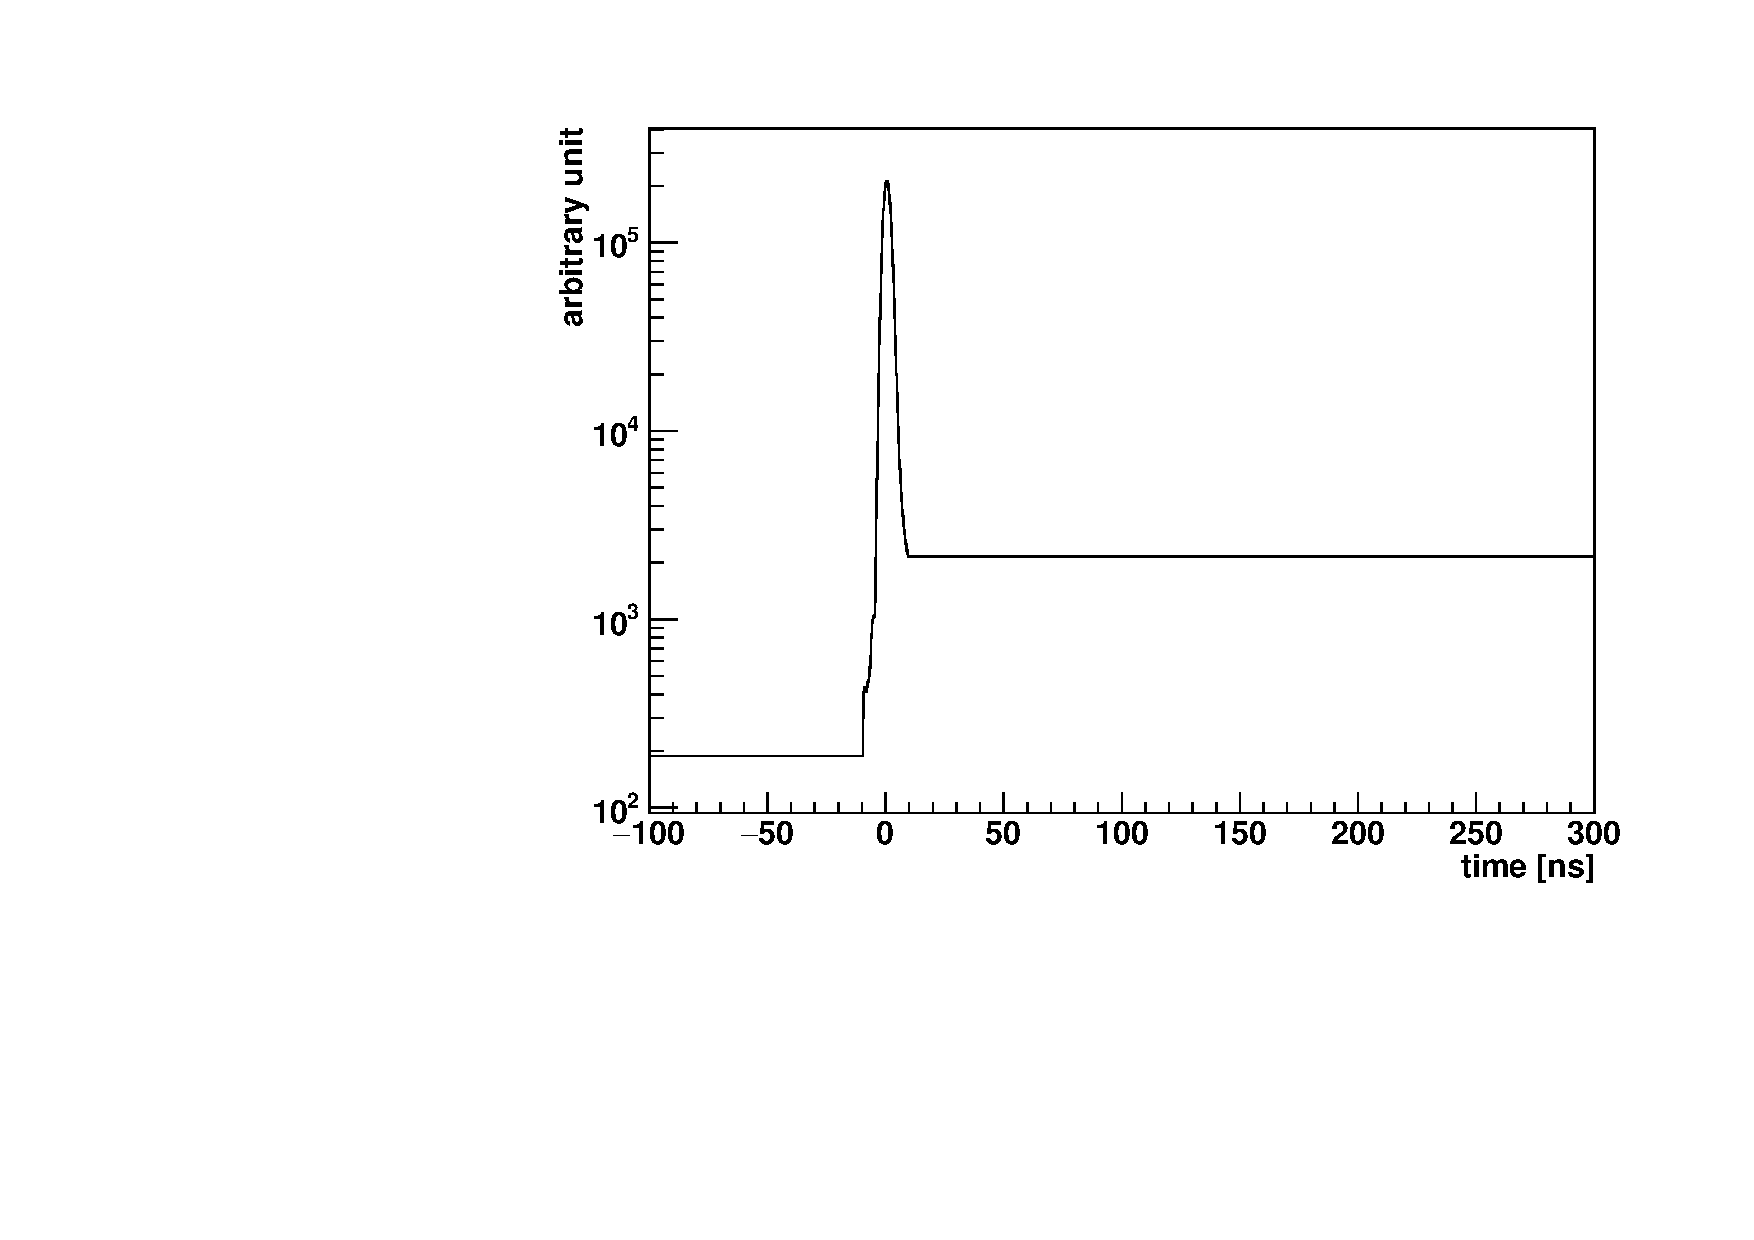
\includegraphics[width=10cm]{MPW_timingPDF.pdf}
	\caption{PMT response time as the timing $PDF$ for the vertex reconstruction.}
	\label{fig:MPW_timingPDF}
\end{figure}

For a trial vertex $(\vec{X}_0,t_0)$, the fitter calculates a $t_{res}$ value with respect to each hit PMT. Looping over all the hit PMTs, a likelihood function is built as:
\begin{equation}\label{eq:vertexLogL}
\ln\mathcal{L}(\vec{X}_0,t_0)=\sum_{i=1}^{{\mathrm{Nhits}}}\ln P(t^i_{res}),
\end{equation}
where $t^i_{res}$ is the time residual calculated from the $i^{th}$ hit PMT; $\mathrm{Nhits}$ is the total number of the hit PMTs triggered by an event and $P(t^i_{res})$ is the probability returned by reading the $PDF$ when given a $t^i_{res}$ for the $i^{th}$ hit PMT.

Therefore, the likelihood function starts with a random ($\vec{X}_0,t_0$) as a seed and calculates the likelihoods and their derivatives for various paths assuming straight line paths of the prompt Cherenkov light from the trial vertex $(\vec{X}_0,t_0)$ to each of the hit PMTs. The trial vertex is varied until the likelihood function reaches the global maximum when the best-fit vertex is found.

This fitting scheme is tackled by the Levenberg-Marquardt (MRQ) method, which is commonly used for fitting the nonlinear model with multiple parameters. This method is described in details in the Sect.~\ref{appendix:MRQ} and its applications for the \texttt{MP fitter} framework is also described. Also see Ref.~\cite{gregory2005bayesian, press2007numerical} for details.

As will be shown in the following sections, one of the main tasks for the fitter is to calculate the $t_{transit}$ by evaluating light paths. In the water phase, both of the AV and cavity were filled with the same ultra-pure water, which is the simplest situation. While in the other situations when the AV is filled with the wavelength shifter or scintillator, since they are different materials with the cavity water, the light path calculations will be complicated.

\subsection{Direction Reconstruction}\label{sect:waterDirection}
A direction vector $\vec{u}$ can be determined by two parameters: the zenith angle $\theta$ and the azimuth angle $\phi$. Then in the Cartesian coordinate system, it can be written as: 
\begin{equation}
\vec{u}=(\cos\phi\sin\theta,\sin\phi\sin\theta,\cos\theta).
\end{equation}

\begin{figure}[htbp]
	\centering
	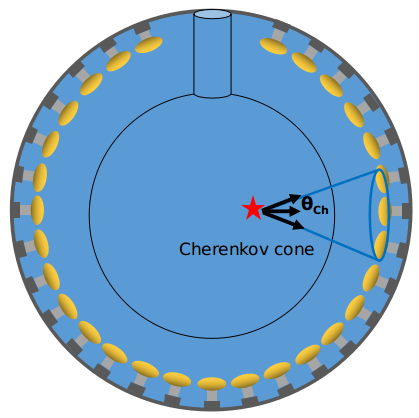
\includegraphics[width=6cm]{mpwDiagram2.png}
	\caption{Diagrams of position in the SNO+ water phase geometry.}
	\label{mpwdiagram_direction}
\end{figure}
To fit for the direction with 2 parameters: $\theta$ and $\phi$, similar to the vertex reconstruction, a random trial direction $\vec{u}_0(\phi_0,\theta_0)$ is generated by using \texttt{CLHEP}, see Sect.~\ref{appendix:random_gen}. The direction fitter then evaluates an angular parameter, $\cos\theta_{\mathrm{Ch}}$, which is the angle between $\vec{u}_{0}$ and $\vec{X}_{{\mathrm{diff}}}\equiv \vec{X}_{event}-\vec{X}_{PMT}$. Therefore, the direction fitter requires an event position as the input and it goes after the vertex fitter\footnote{It has been discussed that, instead of going into two steps, the vertex and direction can be fit simultaneously by utilizing the MRQ algorithm for fitting 6 parameters ($x,y,z,t,\theta,\phi$). However, it shows that the results were worse by using this method.}.

An 1D $PDF$ is used for fitting the angular model, as shown in Fig.~\ref{fig:MPW_angularPDF}. This $PDF$ serves as a model of the angular distributions of the triggered PMTs to an event to be fit. It was obtained from the simulations of 5 MeV $e^-$ events generated at the detector center, i.e., $\vec{X}_{mc}=(0,0,0)$ and traveling along the +x direction, i.e., $\vec{u}_{mc}=(1,0,0)$\footnote{Here 5 MeV is a typical energy for the SNO+ water phase analysis. It also shows that, using the $PDF$s generated by the similar setting but with different $e^-$ energies does minor effect on the reconstruction results.}.

\begin{figure}[!htb]
	\centering
	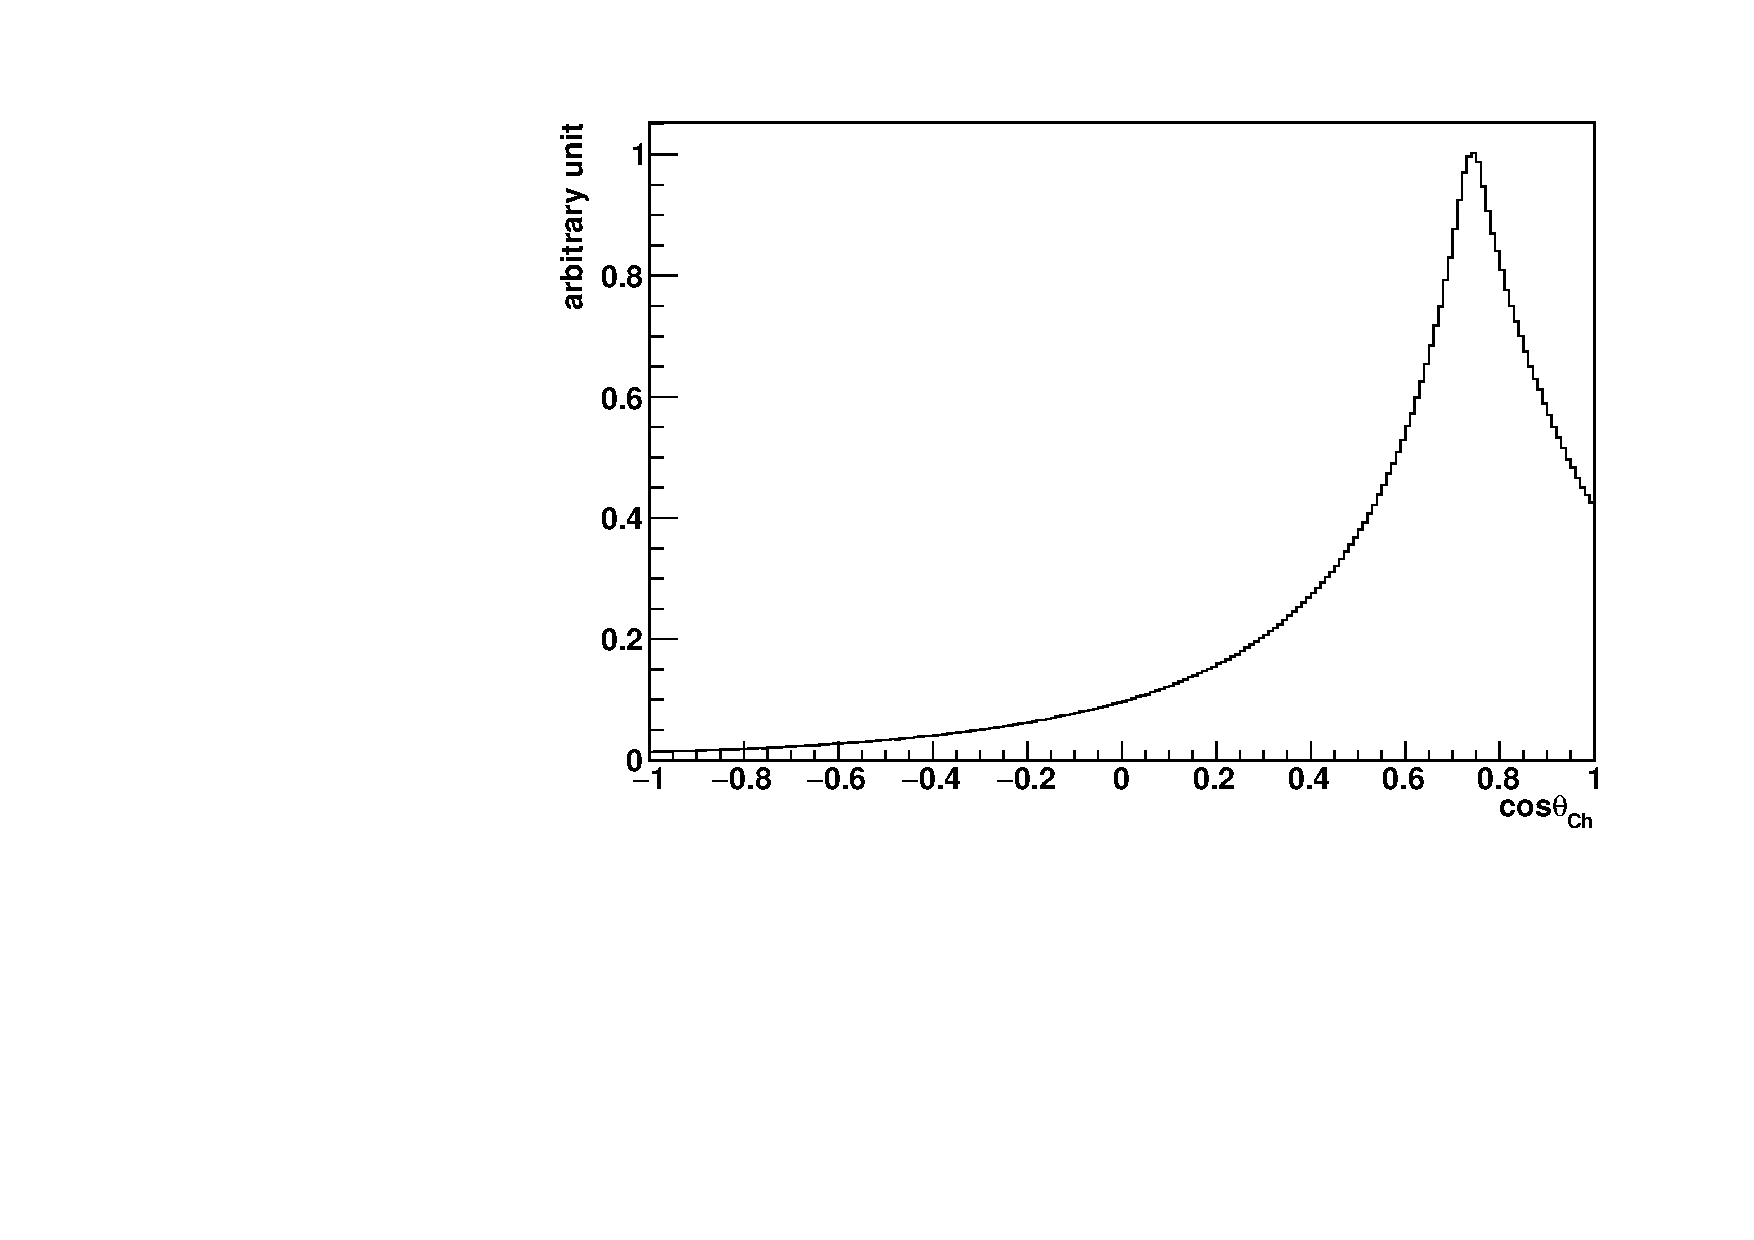
\includegraphics[width=10cm]{MPW_angularPDF.pdf}
	\caption{PMT angular distribution as the angular response $PDF$ for direction reconstruction.}
	\label{fig:MPW_angularPDF}
\end{figure}

For the $i^{th}$ hit PMT, $\cos\theta^i_{\mathrm{Ch}}=\vec{u}_0\cdot\frac{\vec{X}^i_{{\mathrm{diff}}}}{|\vec{X}^i_{{\mathrm{diff}}}|}$, then the likelihood function is built as:
\begin{equation}
\ln L(\vec{u}_0)=\sum_{i=1}^{{\mathrm{Nhits}}}L_i(\cos\theta_{\mathrm{Ch}}^i),
\end{equation}

Finally, the fitter fits for the angular $PDF$ by using the MRQ method to obtain the best-fit direction.

\subsection{Effective Group Velocity}\label{sect:tuneGroupVelocity}
When photons travel through the detector, their group velocities change with different refractive indices of different detector materials. The group velocities also depend on the wavelengths of the photons as $v_g=c/n(\lambda)$. Fig~.\ref{nVsWavelength} shows the measured refractive indices as a function of wavelength, obtained from the measurements of laserball scans in the SNO+ water phase\cite{laserball_groupVelocity}. Furthermore, the group velocities can change when these photons are scattered, absorbed, refracted and reflected. To simplify these complicated situations for the reconstruction, an averaged value of the group velocity is used in the straight line light path calculation. This fixed group velocity is considered as an effective value.

\begin{figure}[!htb]
	\centering
	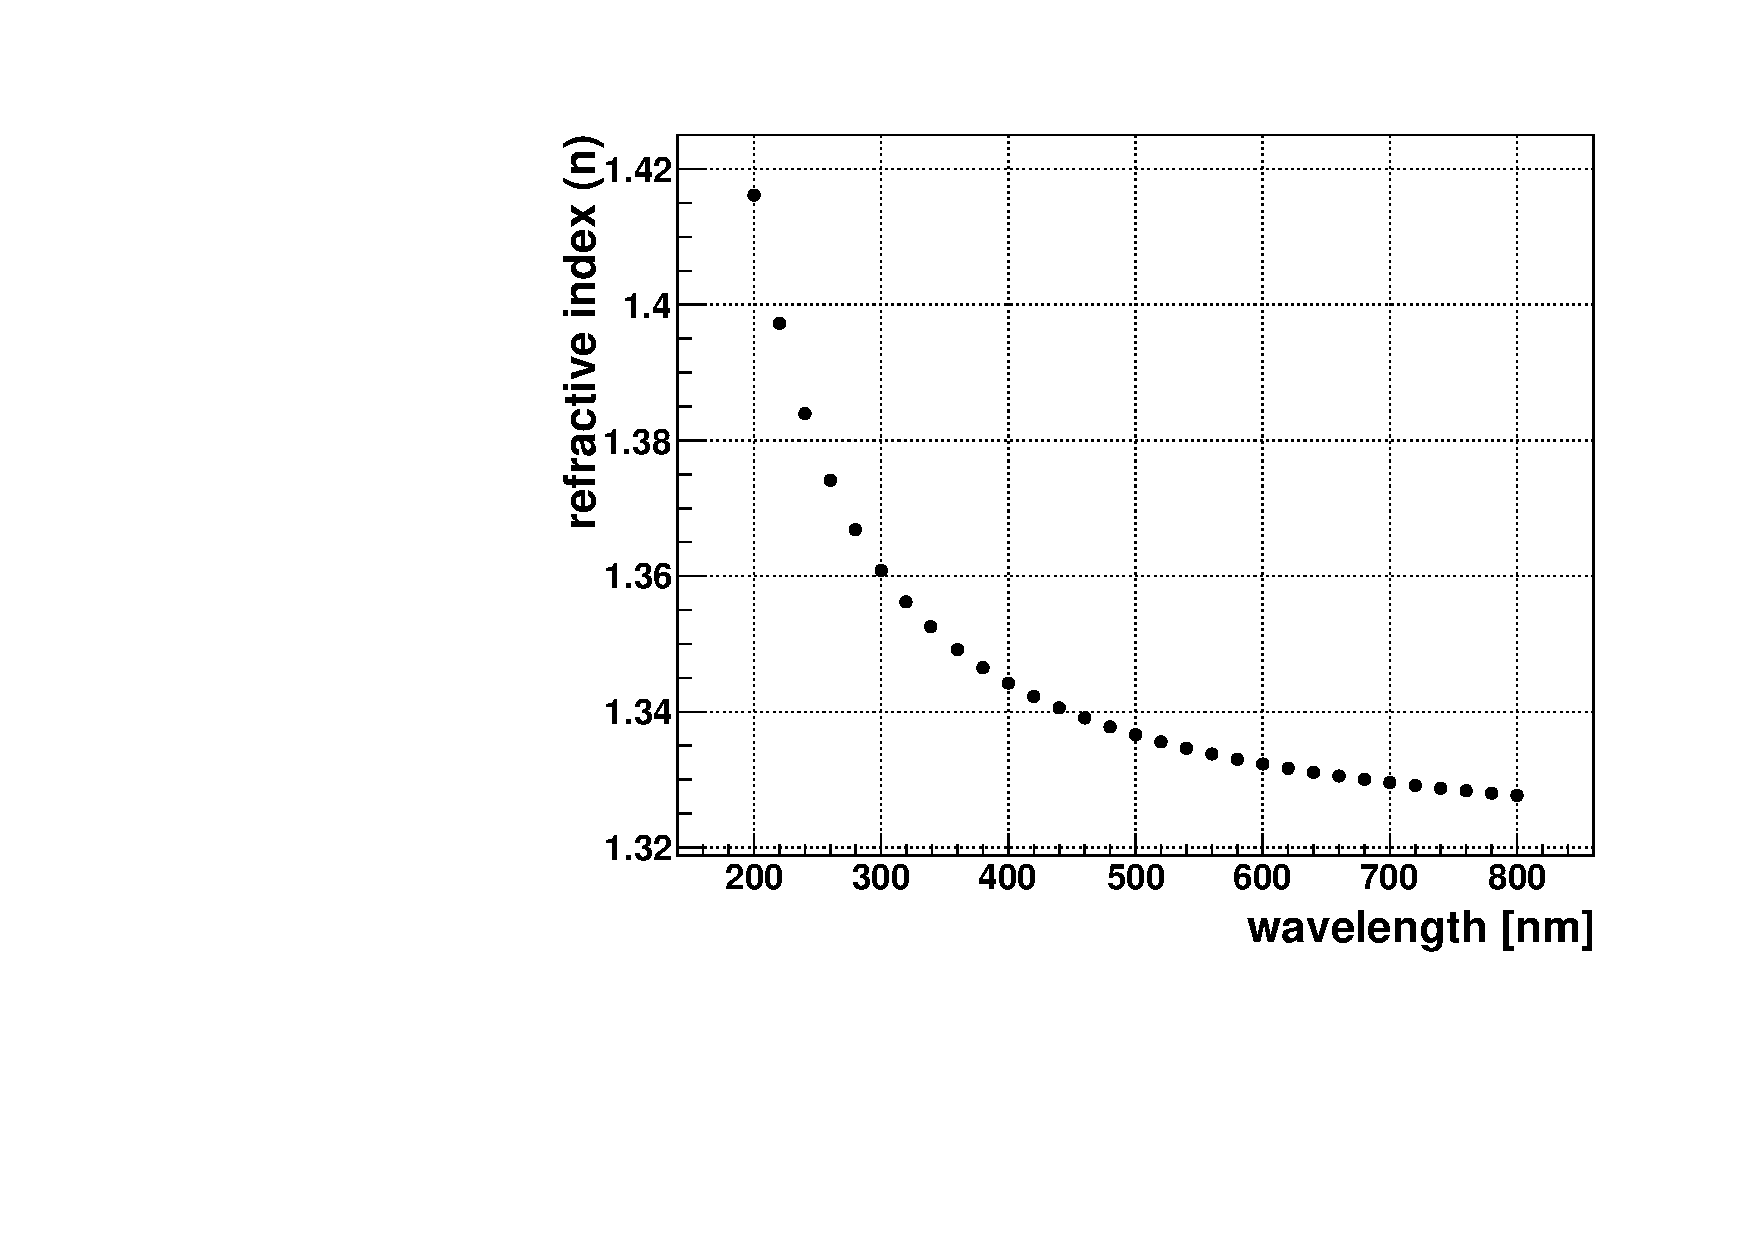
\includegraphics[width=6cm]{refractiveIndexVsWavelength.pdf}
	\caption{Refractive index vs wavelength. These values are based on the measurements from laserball calibration scans in the SNO+ water phase\cite{laserball_groupVelocity}.}
	\label{nVsWavelength}
\end{figure}

A reasonable selection of this value is required, since the value can introduce biases in the fitted position. This kind of bias is mainly due to a ``complementary'' effect of the fitter. As mentioned in section \ref{sect:mpw}, the water vertex fitter calculates the $t_{transit}$ by evaluating the distances from the trial vertex to the hit PMTs: $t_{transit}=|\vec{x}_{event}-\vec{x}_{PMT}|/v_{water}$. If the value of the group velocity $v_{water}$ is set large (or fast speed), the value of $t_{transit}$ will decrease, and the corresponding value of $t_{res}$ will increase according to the definition of $t_{res}$(\ref{tres_define}). These calculated $t_{res}$ value is compared to the time pdf for the fitting. If $t_{res}$ is larger than the expected value, the fitter will place the trial vertex away from the 
hit PMTs to increase the $t_{transit}$ and then decrease the $t_{res}$, as illustrated in Fig.~\ref{effectiveVg}. On the other hand, if $v_{water}$ is set small (or slow speed), $t_{transit}$ increases and $t_{res}$ decreases, and the fitter will place the trial vertex closer towards the hit PMTs.
Therefore, an overestimated group velocity (too fast) brings a positive radial bias to the true event position while an underestimated one (too slow) brings a negative radial bias.
\begin{figure}[!htb]
	\centering
	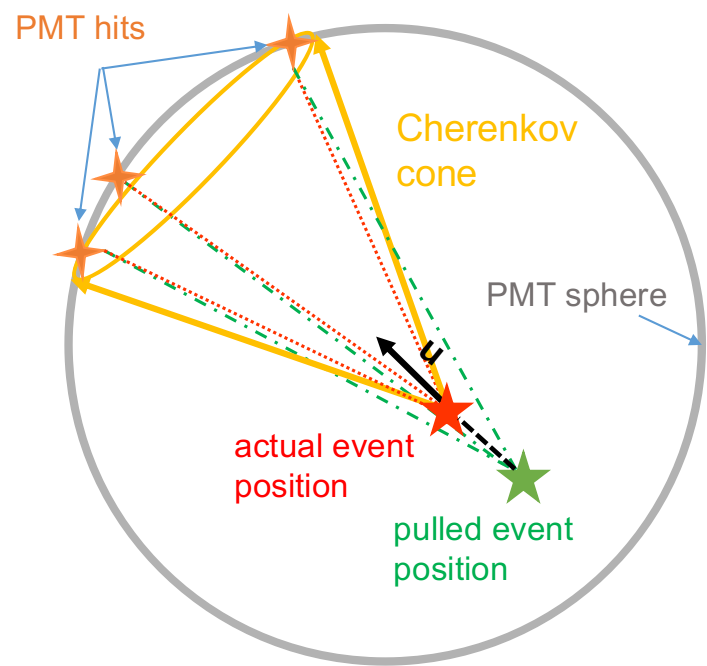
\includegraphics[width=6cm]{effectOfGroupVelocity.png}
	\caption{A cartoon shows effects of tuning the effective group velocity. In this case, the effective group velocity is faster than expected, the fitted position is dragged back along the direction to increase the time of flight.}
	\label{effectiveVg}
\end{figure}

In practice, the effective group velocity is tuned by an effective refractive index $n_{eff}$ (or called $RI$ value): $v_{water}=c/n_{eff}$. To select a reasonable effective group velocity for the water-phase vertex fitter, my first approach is to test on all the values of the refractive index provided by the SNO+ laserball measurements. The values are listed in Fig.~\ref{nVsWavelength}. 

I choose the one which gives the smallest radial bias based on MC simulations. 
For typical 5 MeV $e^-$ events simulated uniformly inside the AV and isotropic momentum,  

As shown in Fig.~\ref{plotGroupV}, $n_{eff}=1.40$ gives the smallest radial bias and is adopt for the MC case.

%\begin{figure}[!htb]
%	\centering
%	\includegraphics[width=6cm]{}
%	\caption{Biases .}
%	\label{plotGroupV}
%\end{figure}

Later I turned to a more data-driven approach rather than tuning from the simulations. This approach is to extract an average group velocity by analyzing the $^{16}$N calibration source data. As shown in Fig.~\ref{n16_groupVeloctiy}, for the $^{16}$N central run-100934 and run-107055, the source was deployed almost at the PSUP center where the optical photons were created and propagated to reach the PMTs on the PSUP. 

For each event, suppose triggered PMTs were found within a solid angle $\Omega$ , 

since the diameter of the PMT concentrator is 27 cm, a line segment $L = 50~cm$ was chose to let the $\Omega$ to include roughly 2 PMTs on the PSUP.
extends with $\theta=\arcsin(L/r_{PSUP})\approx 3.42^\circ$.

the arrival time $T_1$
$\Omega'$, which is the solid angle directly opposed to the $\Omega$, the arrival time $T_2$.

Then the average group velocity was calculated as:
\begin{equation}
v_{gr}=\frac{2 r_{PSUP}}{(T_1+T_2)}.
\end{equation}

This analysis found the $v_{gr}=c/n_{water,eff}=216.478~mm/ns$, where $n_{water,eff}=1.38486$.

\begin{figure}[!htb]
	\centering
	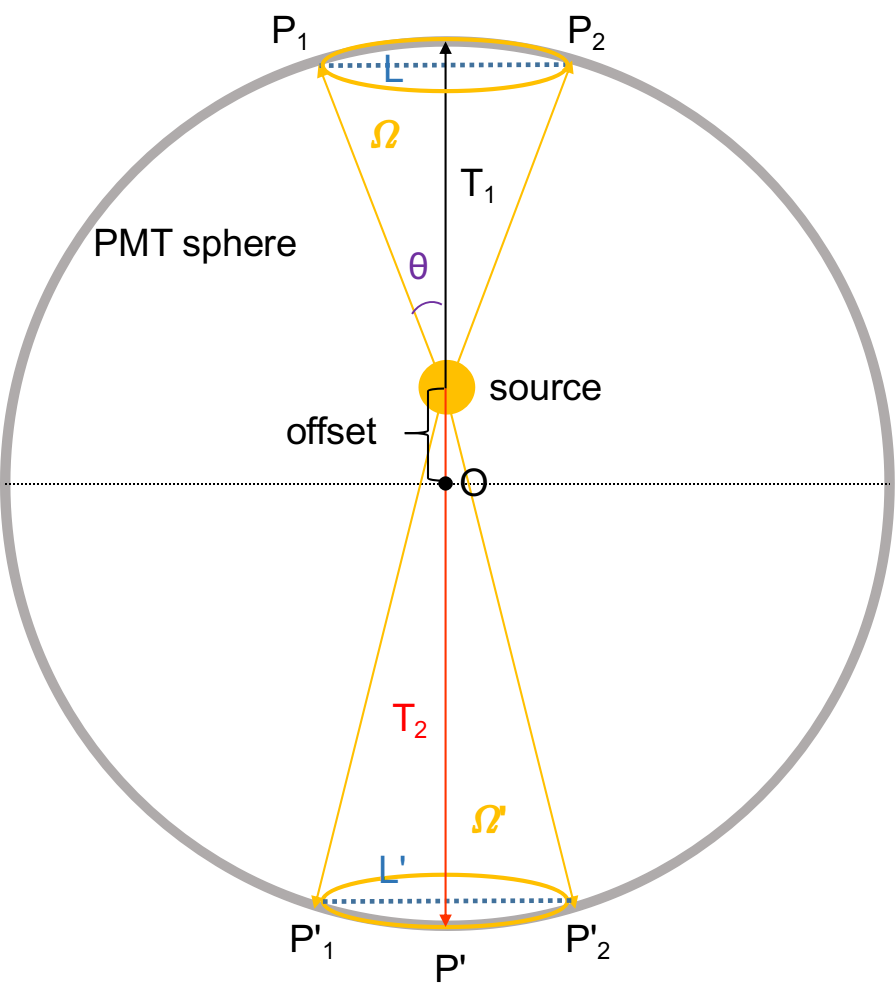
\includegraphics[width=6cm]{n16_groupVelocity.png}
	\caption{$^{16}$N central run for evaluating the average group velocity.}
	\label{n16_groupVeloctiy}
\end{figure}

The SNO+ collaboration used a more complicated approach to measure actual group velocities in the SNO+ water detector by analyzing a set of laserball calibration runs\cite{groupVmeasure,anderson2021optical}.

For the scintillator and partial-fill phase vertex fitters, I adopt a linear interpolation method described in \cite{coulter2013modelling}, which will be discussed in section \ref{sect:scintFitter}.

\subsection{Fitter Pull and Drive Correction}\label{sect:fitterPull}

An effect of ``fitter pull'' in the event vertex reconstruction utilizing the Cherenkov light was observed in the SNO experiment. The distribution of $(\vec{x}_{fit}-\vec{x}_mc)/|\vec{x}_{fit}-\vec{x}_mc|\cdot \vec{u}$ shows a large peak at +1, which indicates that the fitted position $\vec{x}$ is prone to be pulled forward from the true position systematically along the event direction$\vec{u}$\cite{driveCorPeter,brice1996monte,coulter2013modelling}. 

In the SNO+ water detection medium (or the SNO heavy water), Cherenkov photons created by an event trigger most of the PMT-hits with early timing and these hits are located within the Cherenkov cone; for the same event, there are also a few PMT-hits with later timing. These PMT hits can be caused by the scattered or reflected photons and they are located throughout the detector. For a random PMT hit, it is more probable to be placed outside the Cherenkov cone due to the geometry: consider an event happens at the center of the PSUP, the Cherenkov cone it produced will intersect the PSUP by an area of $2\pi R^2_{PSUP}(1-\cos41^\circ)$, which occupies about 12\% of the total area of the PSUP sphere. Therefore, for a random PMT-hit on the PSUP sphere, it has more than 88\% of chance to be placed outside the Cherenkov cone. 

For these later timing PMT hits, a similar ``complementary'' effect mentioned in \ref{tuneGroupVelocity} can also happen. When the fitter fits with $t_{res}$, for the large $t_{res}$ values caused by the later timing hits, it pulls the trial position away from the later timing hits to increase $t_{transit}$ and decrease $t_{res}$, as illustrated in Fig.~\ref{fitterPull}. This effect was also explained as ``straighten out delayed photons'' by the timing fitter in \cite{driveCorPeter}. Furthermore, the major early hits can also cause small $t_{res}$ values and thus the fitter pulls the trial position closer towards the early hits to decrease $t_{transit}$ and increase $t_{res}$. Recall that the early hits are located on or around the Cherenkov cone, therefore an overall effect of this ``fitter pull'' is that the fitted position will be pulled along the axis of the Cherenkov cone and towards the PSUP sphere. This pull direction is coincident with the event direction.

\begin{figure}[!htb]
	\centering
	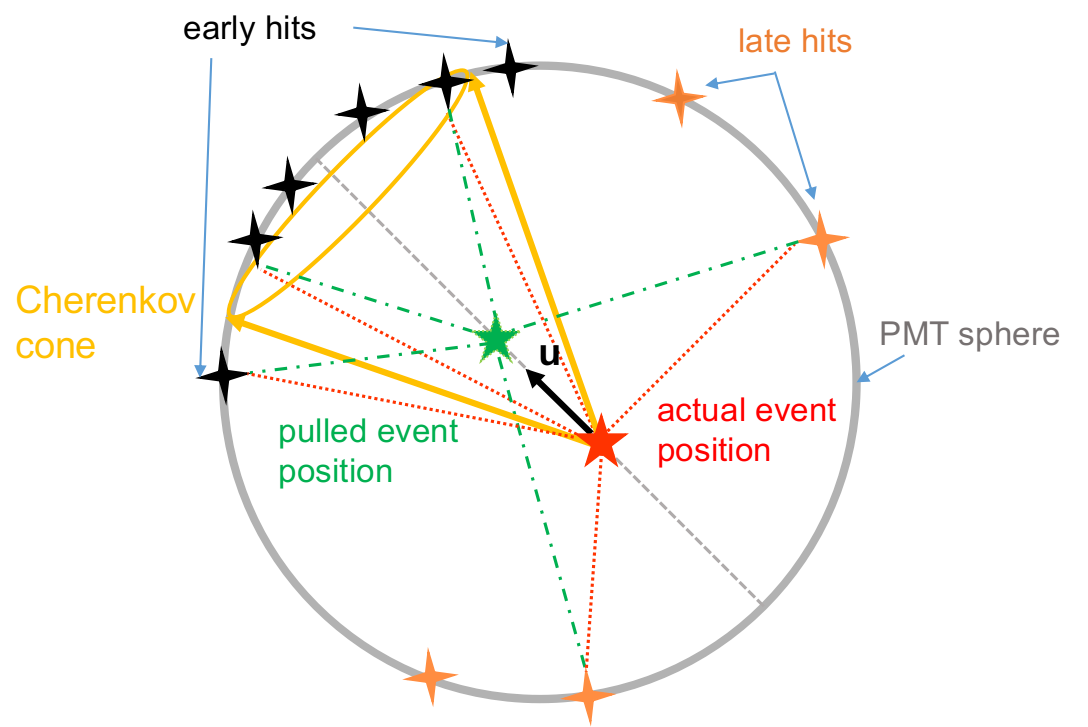
\includegraphics[width=8cm]{fitterPull.png}
\caption{ A cartoon shows fitter pull effect, modified from Fig.~C.2 in \cite{brice1996monte} and Fig.~2,3,4 in \cite{driveCorPeter}.}
	\label{fitterPull}
\end{figure}

A simple way to eliminate this ``fitter pull'' effect is to pull back the fitted event position against the event direction. This is called ``drive correction''.   

Once the \texttt{MPW fitter} obtains both of the fitted position and direction, the drive correction is applied on the fitted position by $\vec{X}_{\mathrm{corrected}} = p_0\vec{X}_{fit}+p_1\vec{u}_{fit}$, where $p_0$ and $p_1$ are the correction parameters, as shown in Fig.~\ref{drivecor}.
\begin{figure}[!htb]
	\centering
	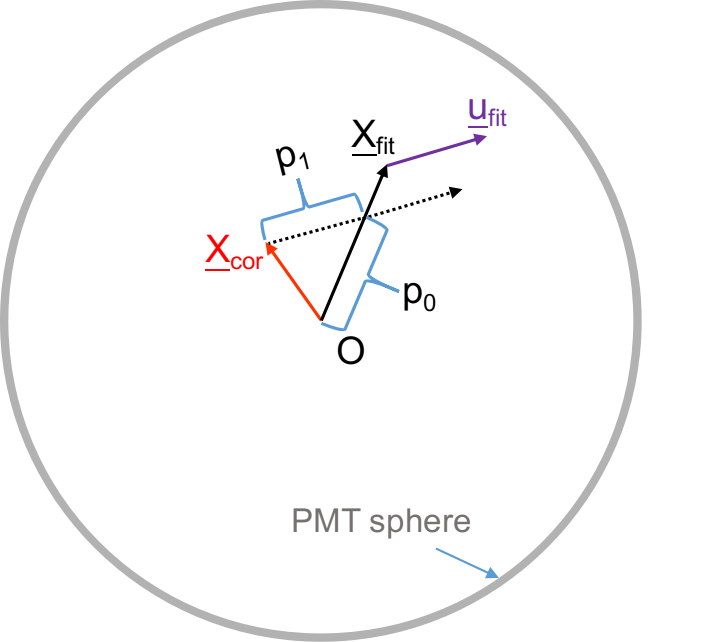
\includegraphics[width=6cm]{driveCor.png}
	\caption{ A diagram illustrates the drive correction.}
	\label{drivecor}
\end{figure}

To obtain the values of $p_0$ and $p_1$, I generated electron events distributed isotropically inside the AV. The simulations of 2, 3, 4, ... ,10 MeV electrons are produced. Then the \texttt{MPW fitter} is applied on each simulations and returns the results of $\vec{X}_{fit}$ and $\vec{u}_{fit}$. Take the Monte Carlo generated positions $\vec{X}_{MC}$ as the true positions, for all the fitted events, a $\chi^2$ function is calculated by:
\begin{equation}
\chi^2 = \sum_{i=1}^{N_{\mathrm{events}}}[\vec{X}^i_{MC}-(p_0\vec{X}^i_{fit}+p_1\vec{u}^i_{fit})]^2,
\end{equation}

The $p_0$ and $p_1$ are obtained by minimizing the $\chi^2$ function. When calculating the $\chi^2$, the fitted events of $|\vec{X}_{fit}-\vec{X}_{MC}|>3~m$ are thrown away to improve the $\chi^2$ minimization results.

For the 2 to 10 MeV electrons simulations, the obtained values of $p_0$ and $p_1$ are energy or Nhit dependent. However, it does not improve the results if using the $\mathrm{NHits}$ dependent functions $p_0(Nhit)$ and $p_1(Nhit)$ as drive corrections.
Finally we take the average values from the 5 to 10 MeV electrons simulations and the drive correction is set as: 
\begin{equation}
\vec{X}_{\mathrm{corrected}} = 0.99577\vec{X}_{fit}+-63.826\vec{u}_{fit}.
\end{equation}

It is important to note that since the drive correction parameters are obtained from the reconstructions of Monte Carlo, it depends on the Monte Carlo and the results of reconstruction. Therefore, the n$_{water}$, mode cut and time residue cut affecting the fitted results will also affect the drive correction parameters, but not significantly.


\begin{figure}[!htb]
	\centering
	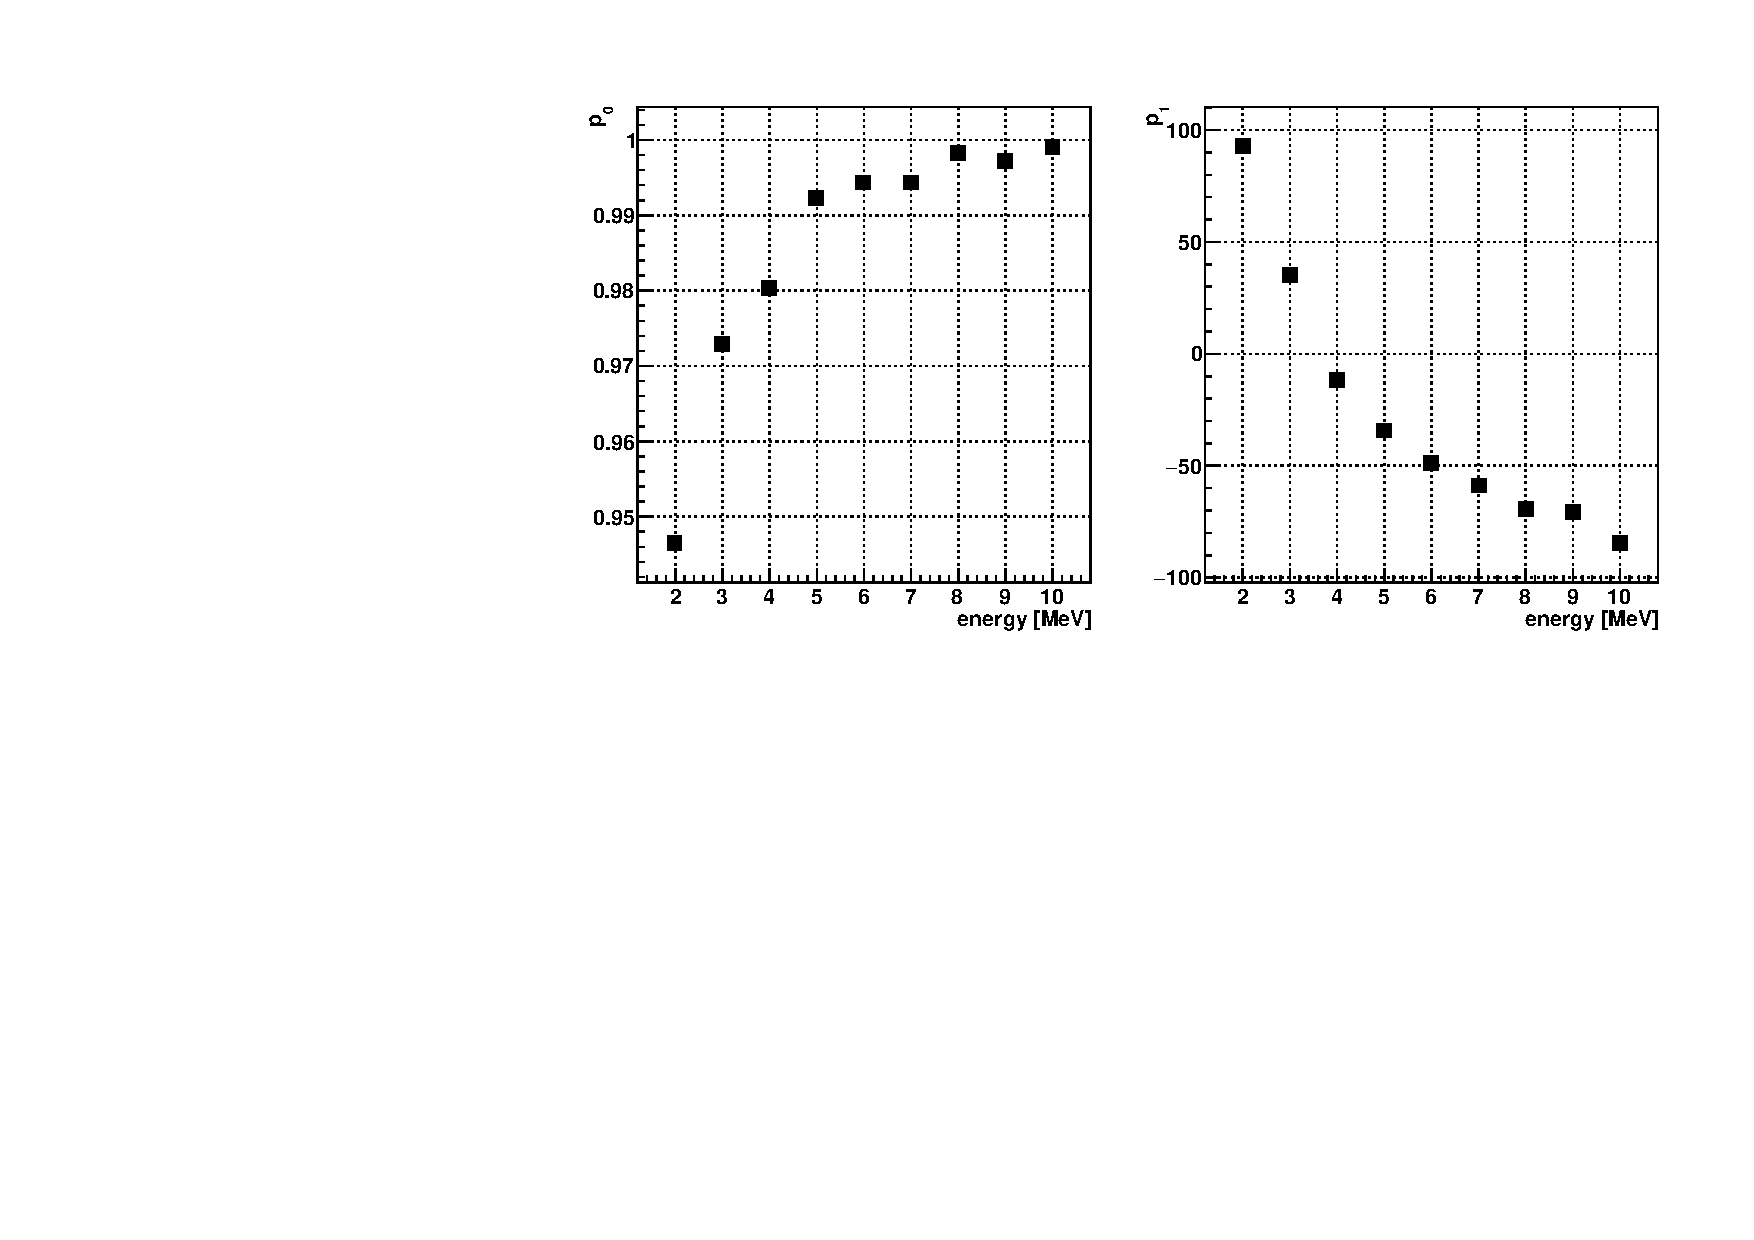
\includegraphics[width=10cm]{pullParVsEnergy.pdf}
	\caption{ Drive correction parameter $p_0$, $p_1$ vs energy.}
	\label{pullParVsEnergy}
\end{figure}

Electron events with various energies were generated at the detector center and their momentum were along +x direction. 

\begin{figure}[!htb]
	\centering
	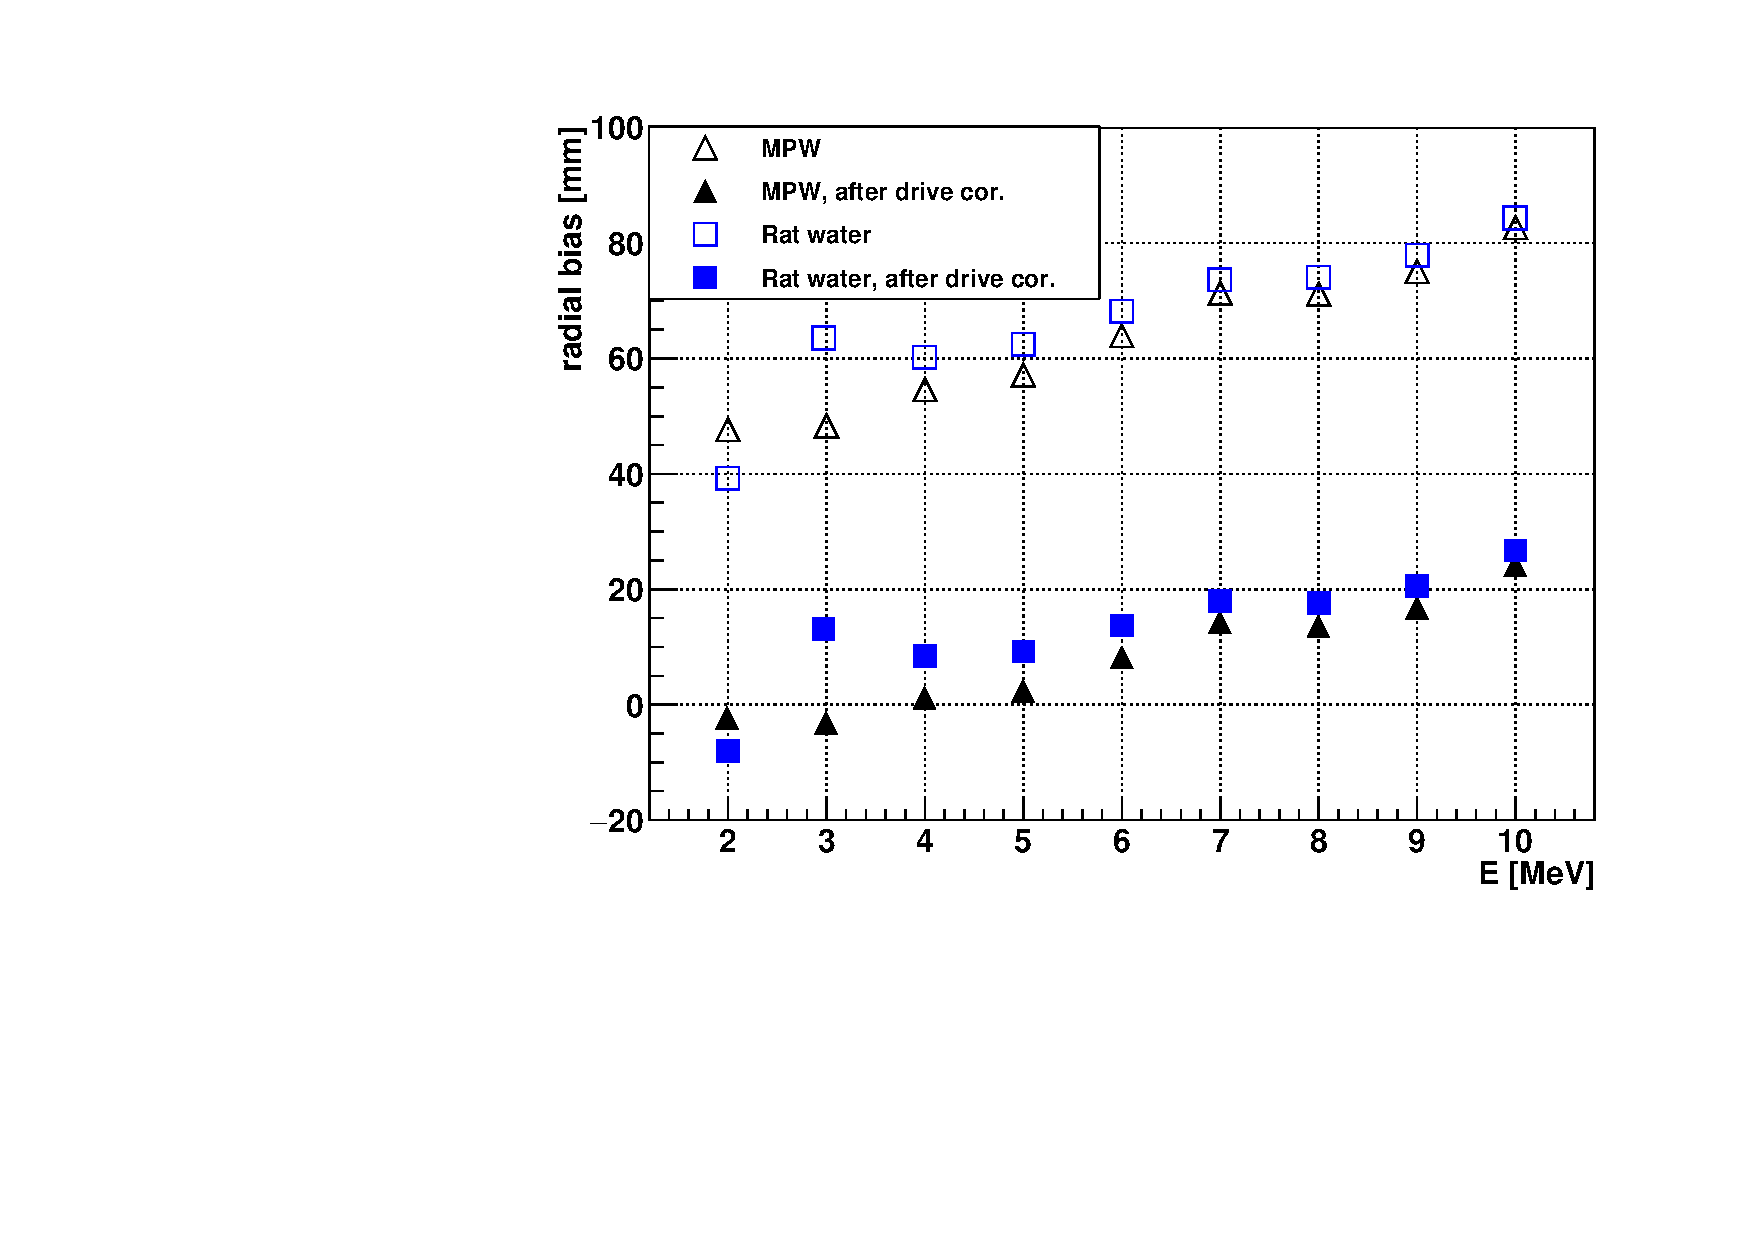
\includegraphics[width=8cm]{pullEffectVsEnergy.pdf}
	\caption{ Radial biases of simulated electron events before and after the drive correction, as a function of energy.}
	\label{drivecorVsEnergy}
\end{figure}

By fitting the simulations of 5 MeV electrons generated at the detector center and traveling along +x direction, the drive effct of the MPW fitter causes a $\sim$50 mm biases from the detector center along +x axis. The drive correction reduces this drive bias down to $\sim$0.2 mm. For the reconstruction of $^{16}$N data, the drive correction can reduce the fitted position RMS by $\sim$20 mm.

\subsection{Water Fitter Performances}

By using the \texttt{RAT} (version 6.5.5) package, 10000 $e^-$ events were generated at the detector center (in the PSUP coordination) with isotropic momentum directions. Default detector trigger settings in the SNO+ water phase were used (\texttt{N100Hi}=21.0,\texttt{N100Med}=16.0 and \texttt{N100Lo}=11.0). With these settings, low energy events may not trigger the detector and thus the number of the reconstructed events can be lower than the simulated events.

Fig.~\ref{fig:5MeVbeta_center_water} shows the position reconstruction results for the 5-MeV $e^-$ events. The fit position biases $\vec{X}_{fit}-\vec{X}_{mc}$ were projected on the x, y and z axes respectively and were filled into 1D histograms which were further fitted with Gaussian functions. Here the Gaussian mean ($\mu$) is regarded as the fit bias while the Gaussian sigma ($\sigma$) is regarded as fit resolution.
\begin{figure}[htbp]
	\centering \label{fig:5MeVbeta_center_water}
	\subfigure[$x_{fit}-x_{mc}$]{
		\begin{minipage}[t]{0.38\textwidth}
			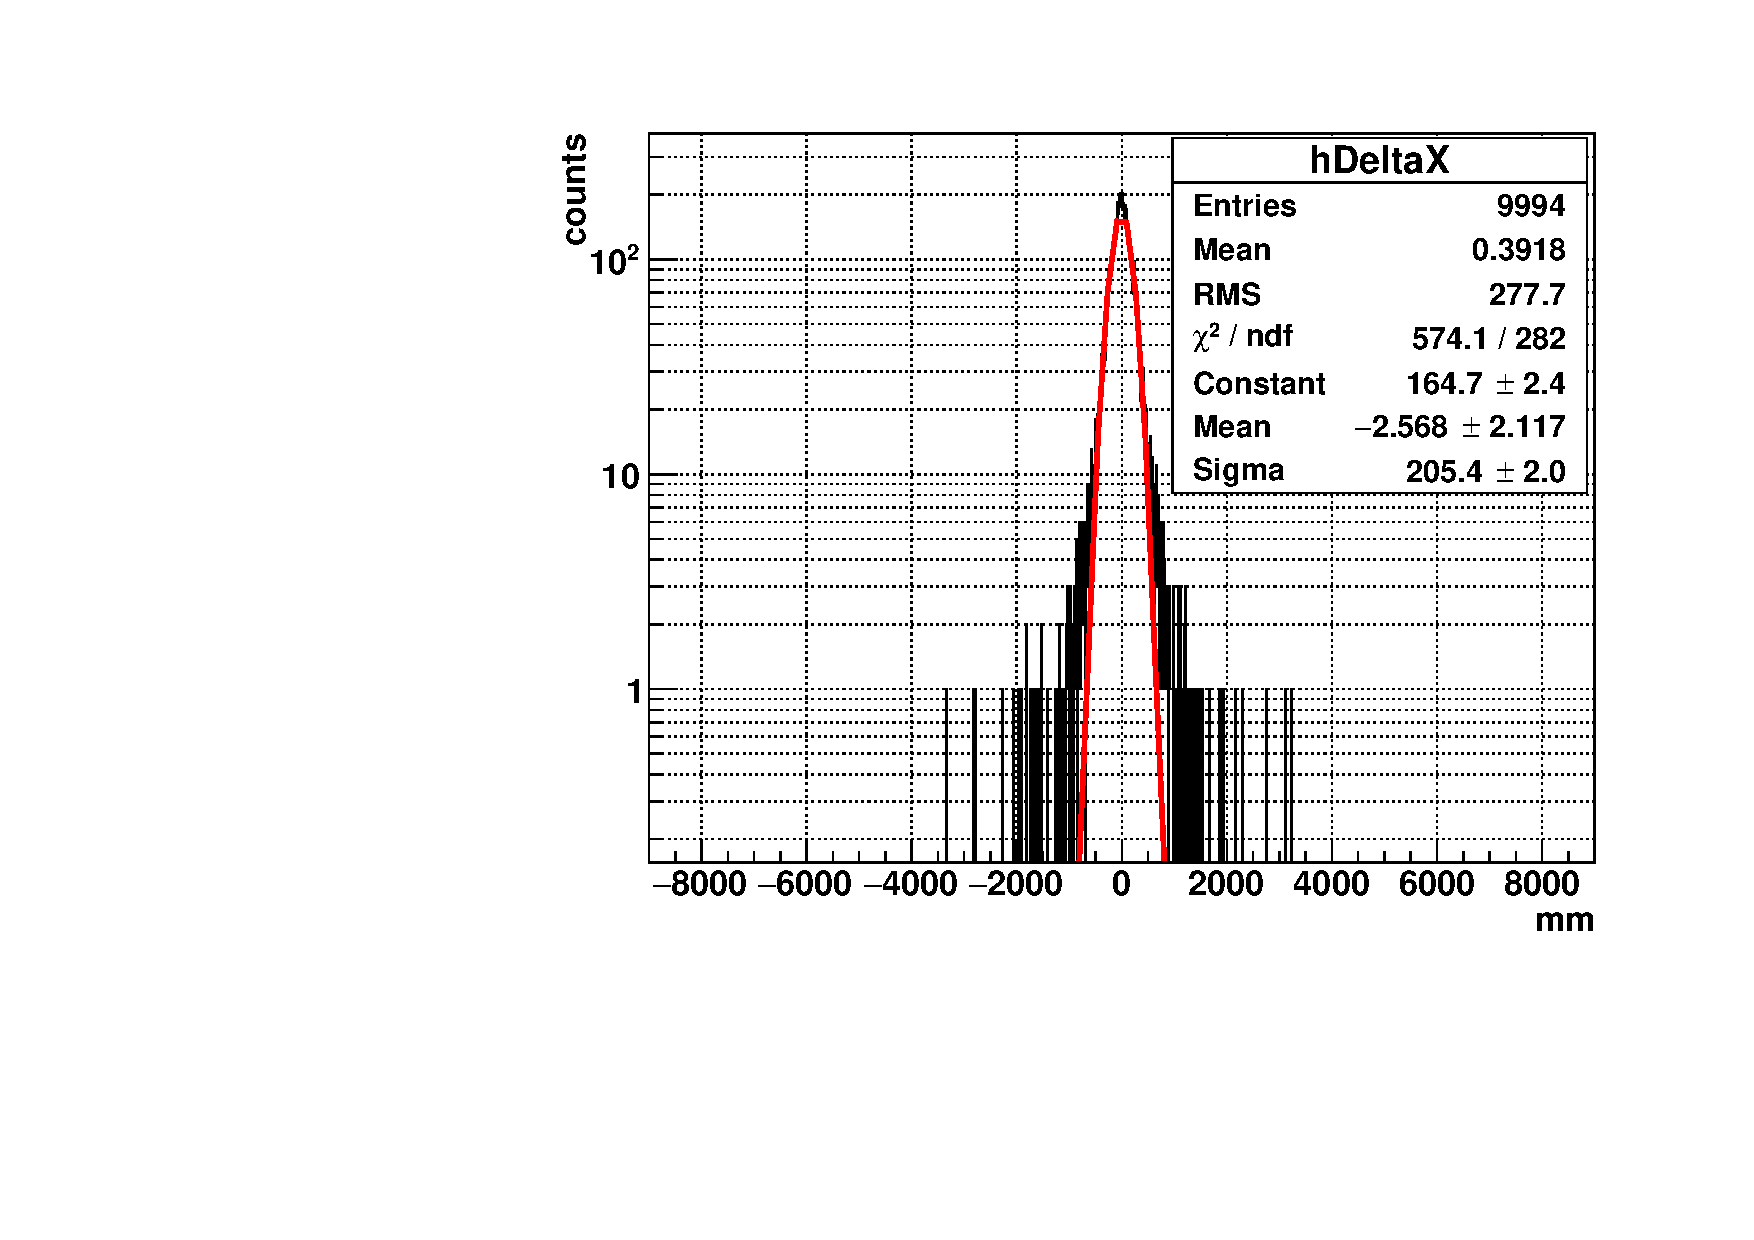
\includegraphics[width=6cm]{5MeVbetaX.png}
		\end{minipage}
	}   
	\subfigure[$y_{fit}-y_{mc}$]{ 
		\begin{minipage}[t]{0.38\textwidth}
			\centering
			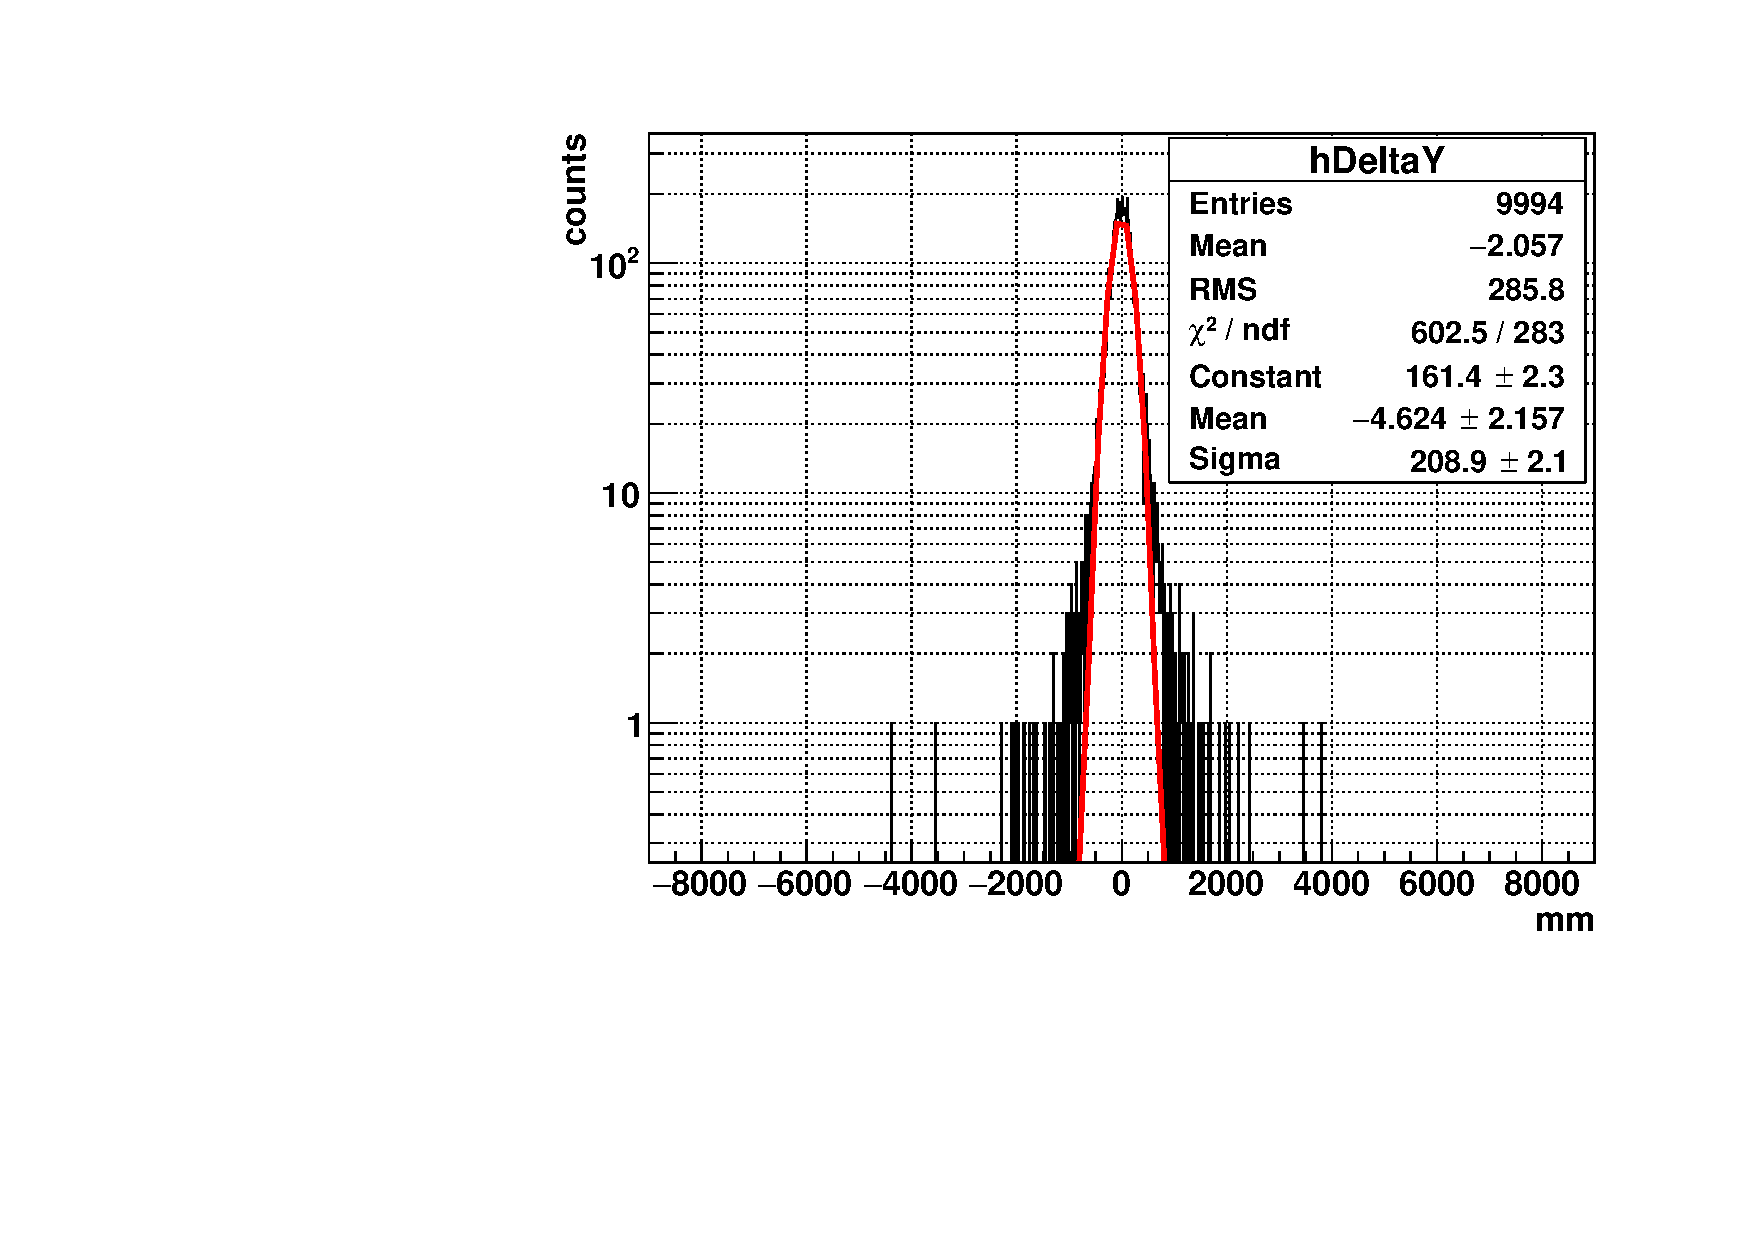
\includegraphics[width=6cm]{5MeVbetaY.png}
		\end{minipage}
	}
	\subfigure[$z_{fit}-z_{mc}$]{ 
		\begin{minipage}[b]{0.32\textwidth}
			\centering
			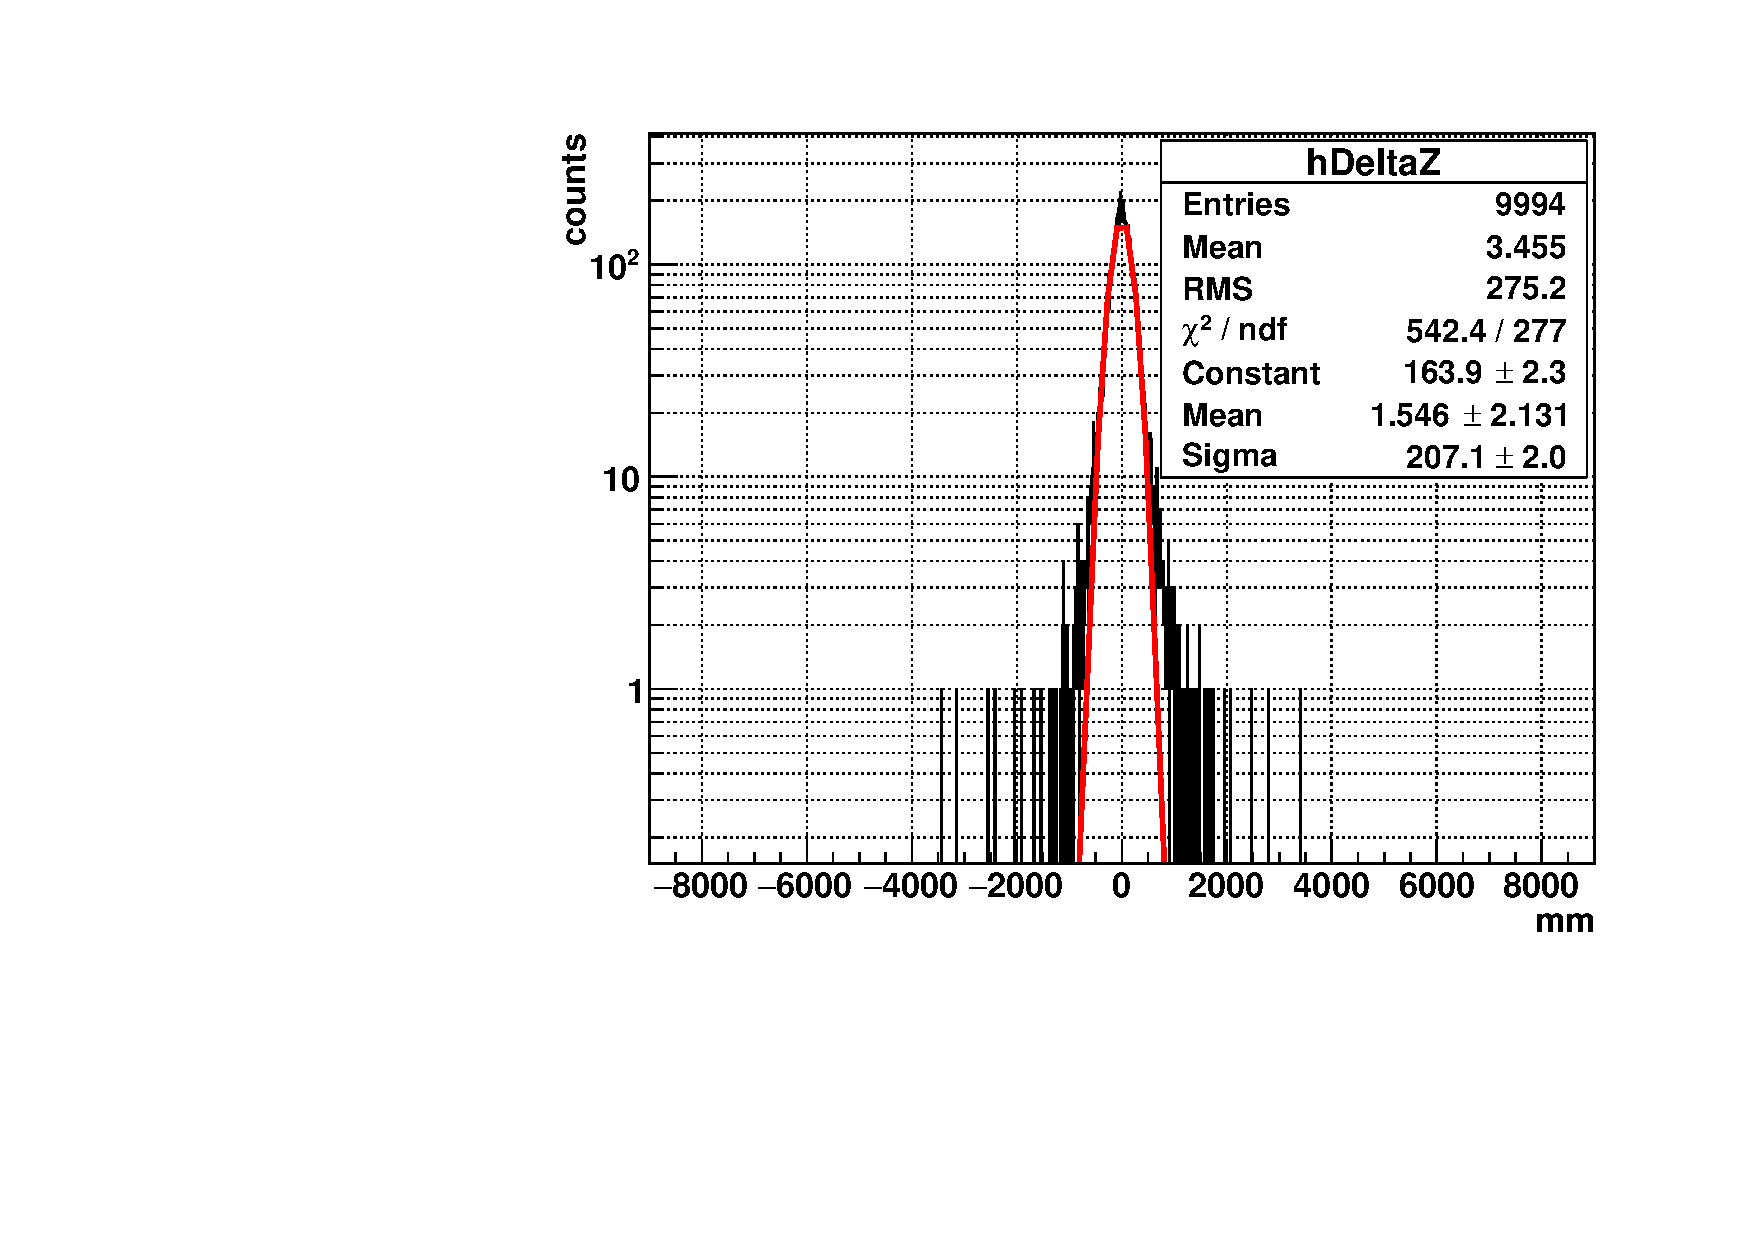
\includegraphics[width=6cm]{5MeVbetaZ.png}
		\end{minipage}
	}
	\caption{Distributions of fit position biases projected on x axis ($x_{fit}-x_{MC}$), for 5-MeV events.}
\end{figure}

The events with the same settings but different energies, from 2 MeV to 15 MeV by a 1 MeV step, were also simulated. Their results are shown in Fig.~\ref{fig:MPWposResol}. It shows that the event with higher energy can produce more photons from the detection medium and thus triggers more PMTs. With a larger NHits, the fitter has more information to fit and can return better position resolutions. As I will show in the following section, for a decent detection medium which can produce more photons for the same event, the position resolution can also be improved.
 
\begin{figure}[htbp]
	\centering	
	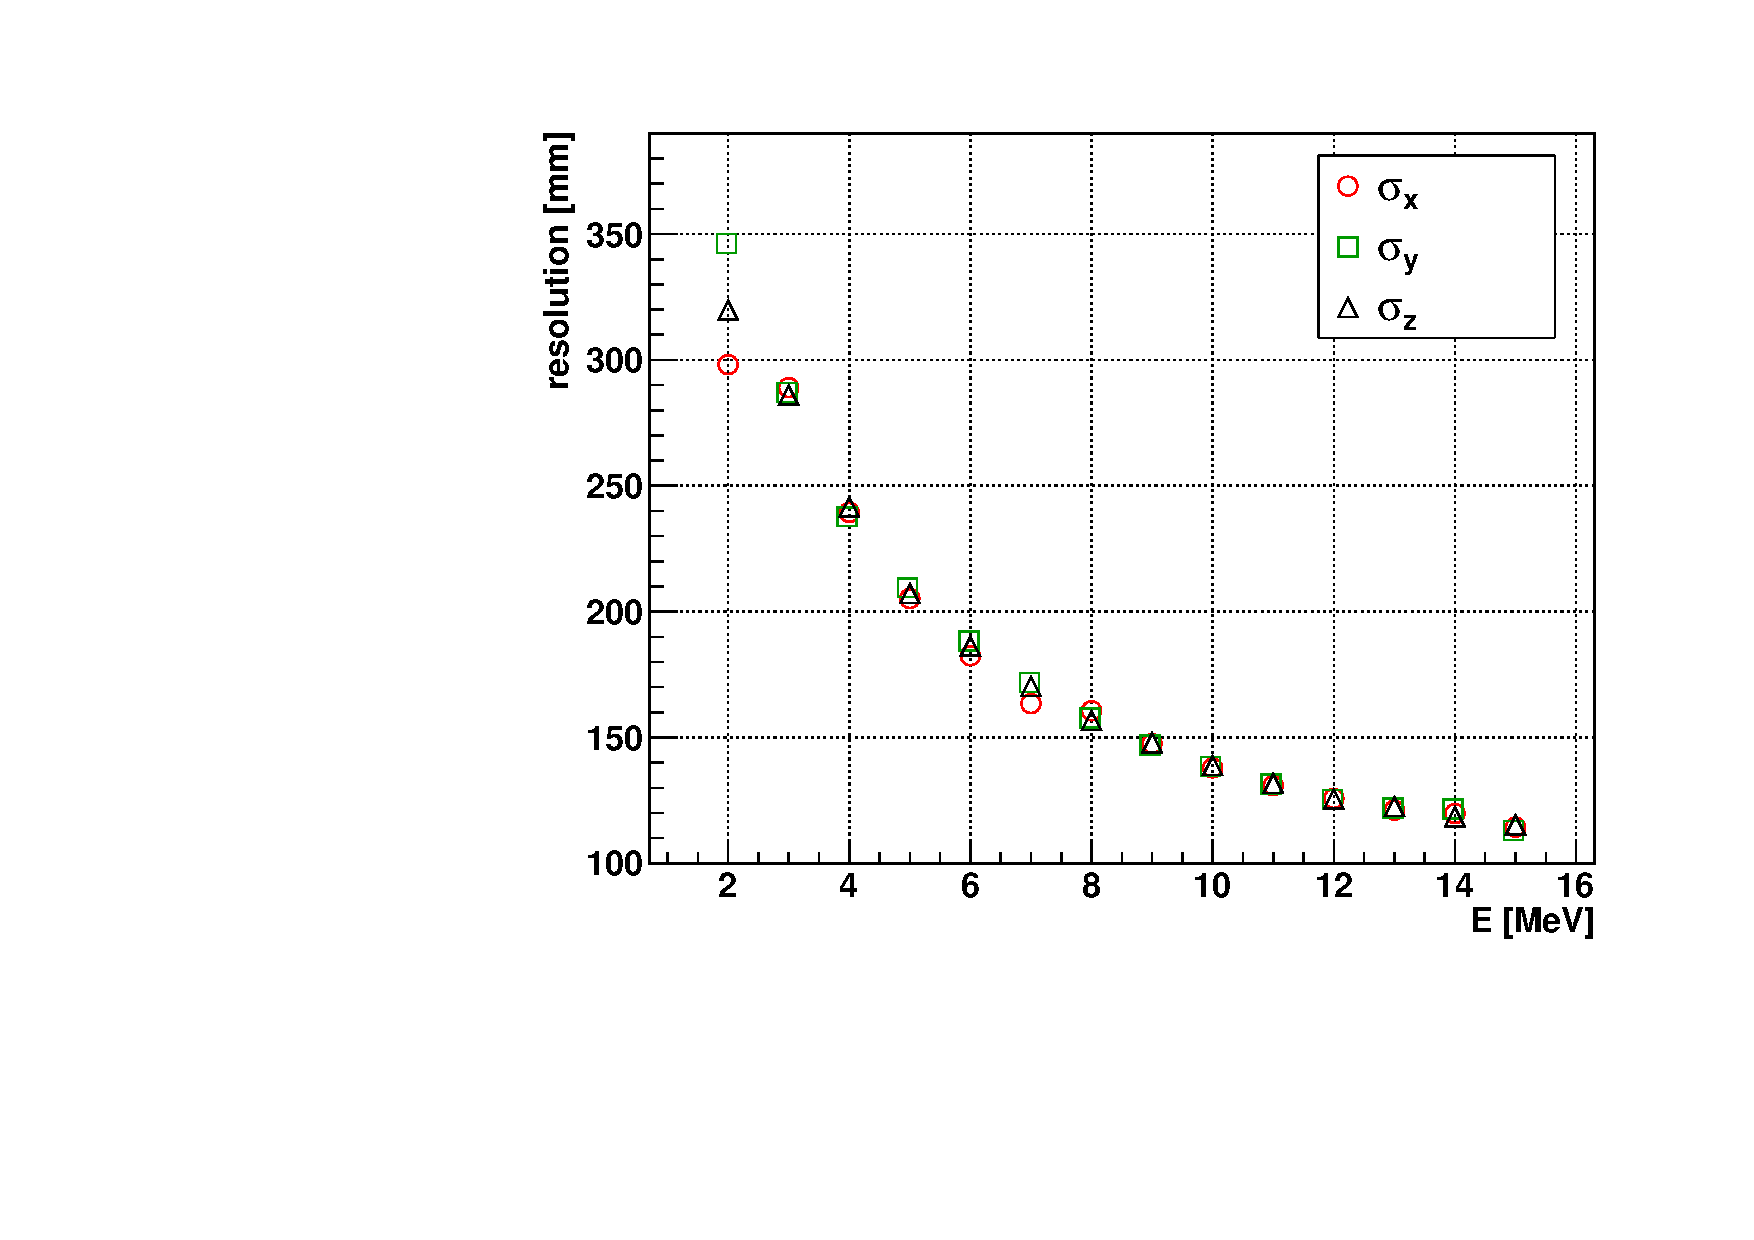
\includegraphics[width=9cm]{MPW_posResolVsE.pdf}
	\caption{The \texttt{MPW fitter} position resolutions of x, y, z axes as a function of energies.}
	\label{fig:MPWposResol}
\end{figure}

A more generic situation is that the events happens everywhere inside the AV. In this simulation, $e^-$ events were generated uniformly inside the AV volume. 

\begin{figure}[htbp]
	\centering	
	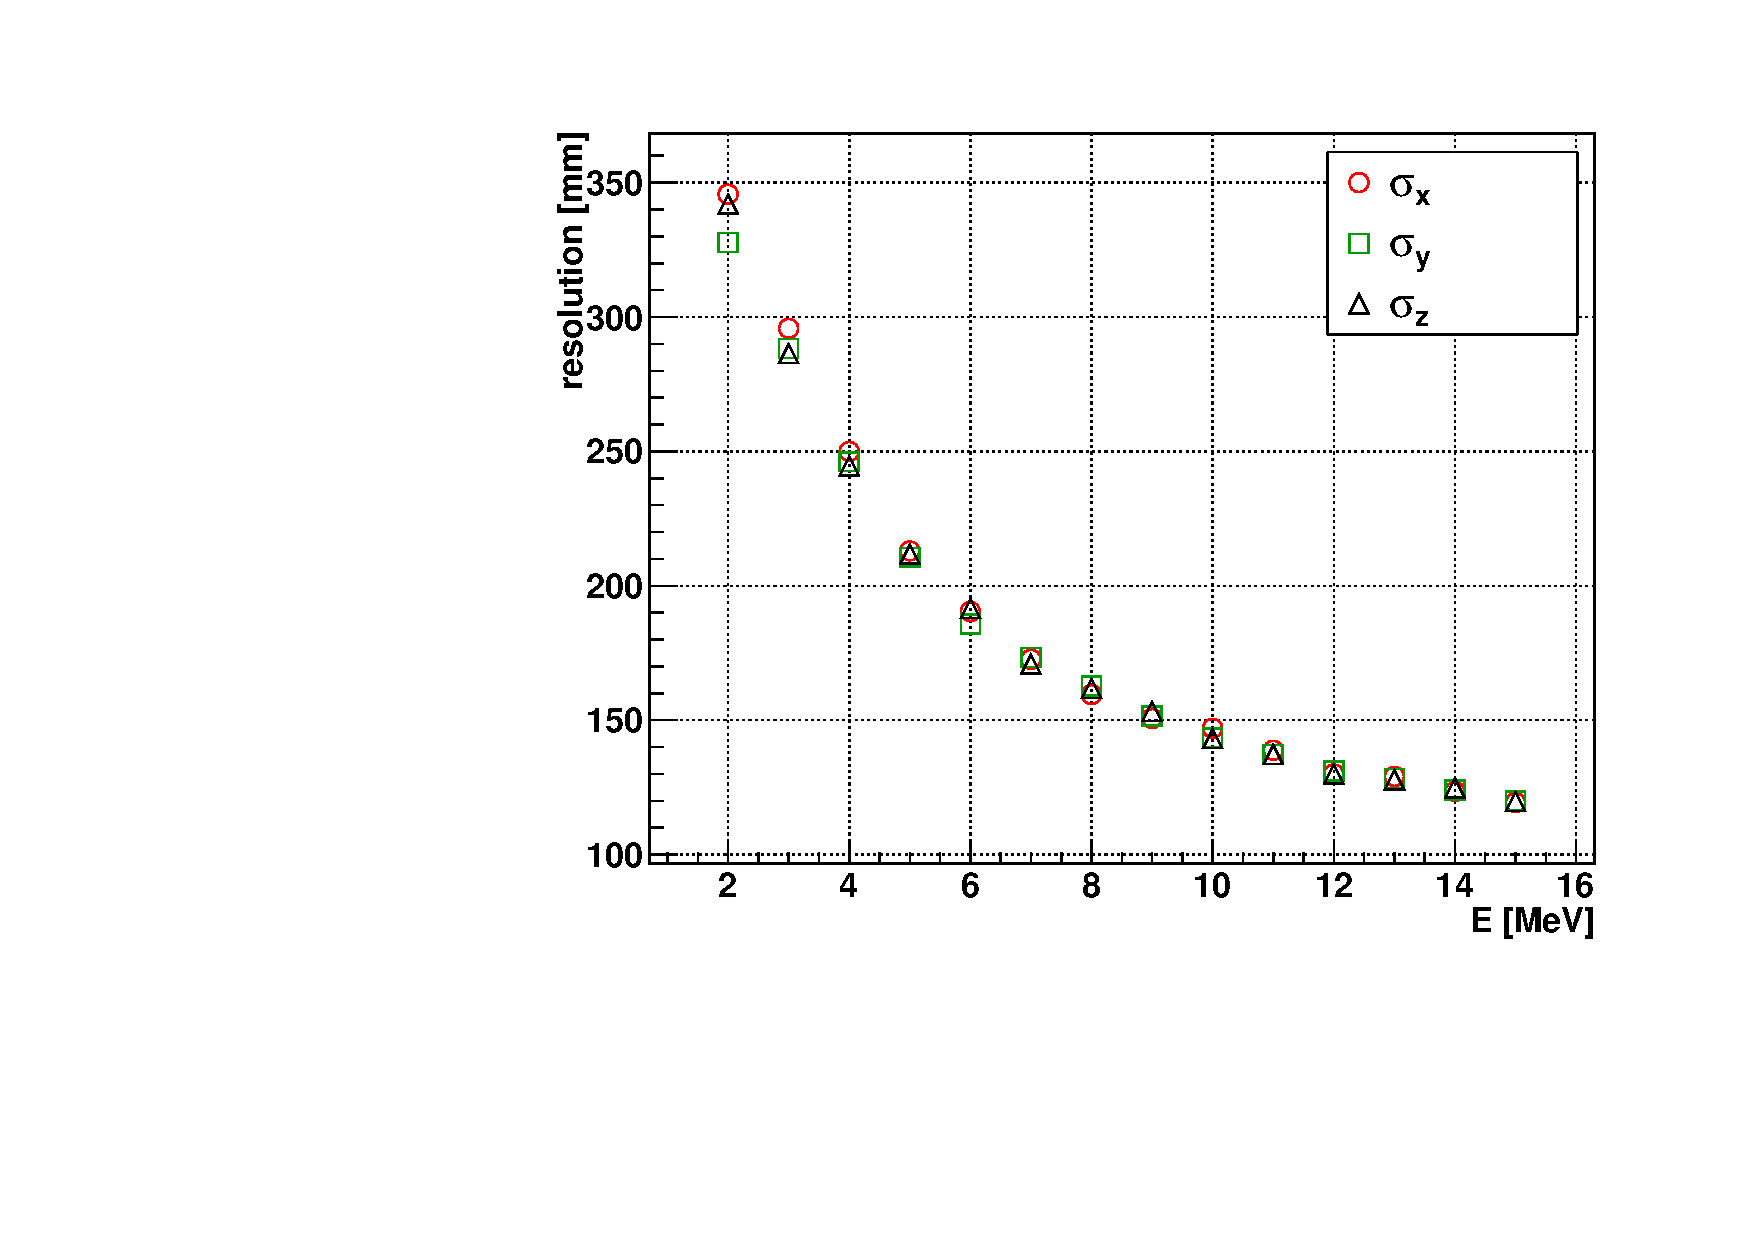
\includegraphics[width=9cm]{MPW_isoFill_posResolVsE.pdf}
	\caption{The \texttt{MPW fitter} position resolutions of x, y, z axes as a function of energies.}
	\label{fig:MPWposResol_isoFill}
\end{figure}
%\begin{table}[ht]
%	\caption{Fitter resolutions in water phase.}\label{table:fitterBiasInWater}
%	\centering		
%	\begin{tabular*}{120mm}{c@{\extracolsep{\fill}}cccc}
%		\toprule 
%		medium & $\cos\theta_{0.9}$ & $\cos\theta_{0.8}$ & $\cos\theta_{0.5}$\\
%		\midrule
%		SNO heavy water  & 0.50 & 0.71 & 0.92  \\	
%		SNO+ water  & 0.53 & 0.76 & 0.93	 \\
%		wbWLS  & 0.37 & 0.63 & 0.90  \\	
%		\bottomrule	
%	\end{tabular*}
%\end{table}

\subsection{Direction Resolutions}\label{sect:directResol}

To describe the biases between the reconstructed direction and the true particle direction of the event, an empirical function for the angular resolution was adopted by SNO\cite{boulay2004direct} and it is defined as a combination of two exponential components:
\begin{equation}\label{eq:directResol}
P(\cos\theta)=\alpha_M\frac{\beta_M\exp[-\beta_M(1-\cos\theta)]}{1-\exp(-2\beta_M)}+(1-\alpha_M)\frac{\beta_s\exp[-\beta_s(1-\cos\theta)]}{1-\exp(-2\beta_s)},
\end{equation}
where the parameters: $\beta_M$ and $\beta_S$ are the ``decay'' constants or the ``slopes'' of the two exponential components; $\alpha_M$ is the fraction between two exponential components. The first component, the main peak is due to the single scattering of the electrons and is the true angular resolution of the detector, while the second component which has a broad tail is mainly due to the multiple scattering of electrons; there are also back scattering electrons on the detector components and the poorly reconstructed events in the tails\cite{boulay2004direct}.

\subsection{Test on Gamma Events}

The $\gamma$ events with energies of 2.2 MeV and 4.4 MeV are crucial for analyzing the AmBe calibration data (see Sect.~\ref{sect:AmBesource}). 

\begin{figure}[htbp]
	\centering
	\subfigure[$x_{fit}-x_{mc}$]{
		\begin{minipage}[t]{0.38\textwidth}
			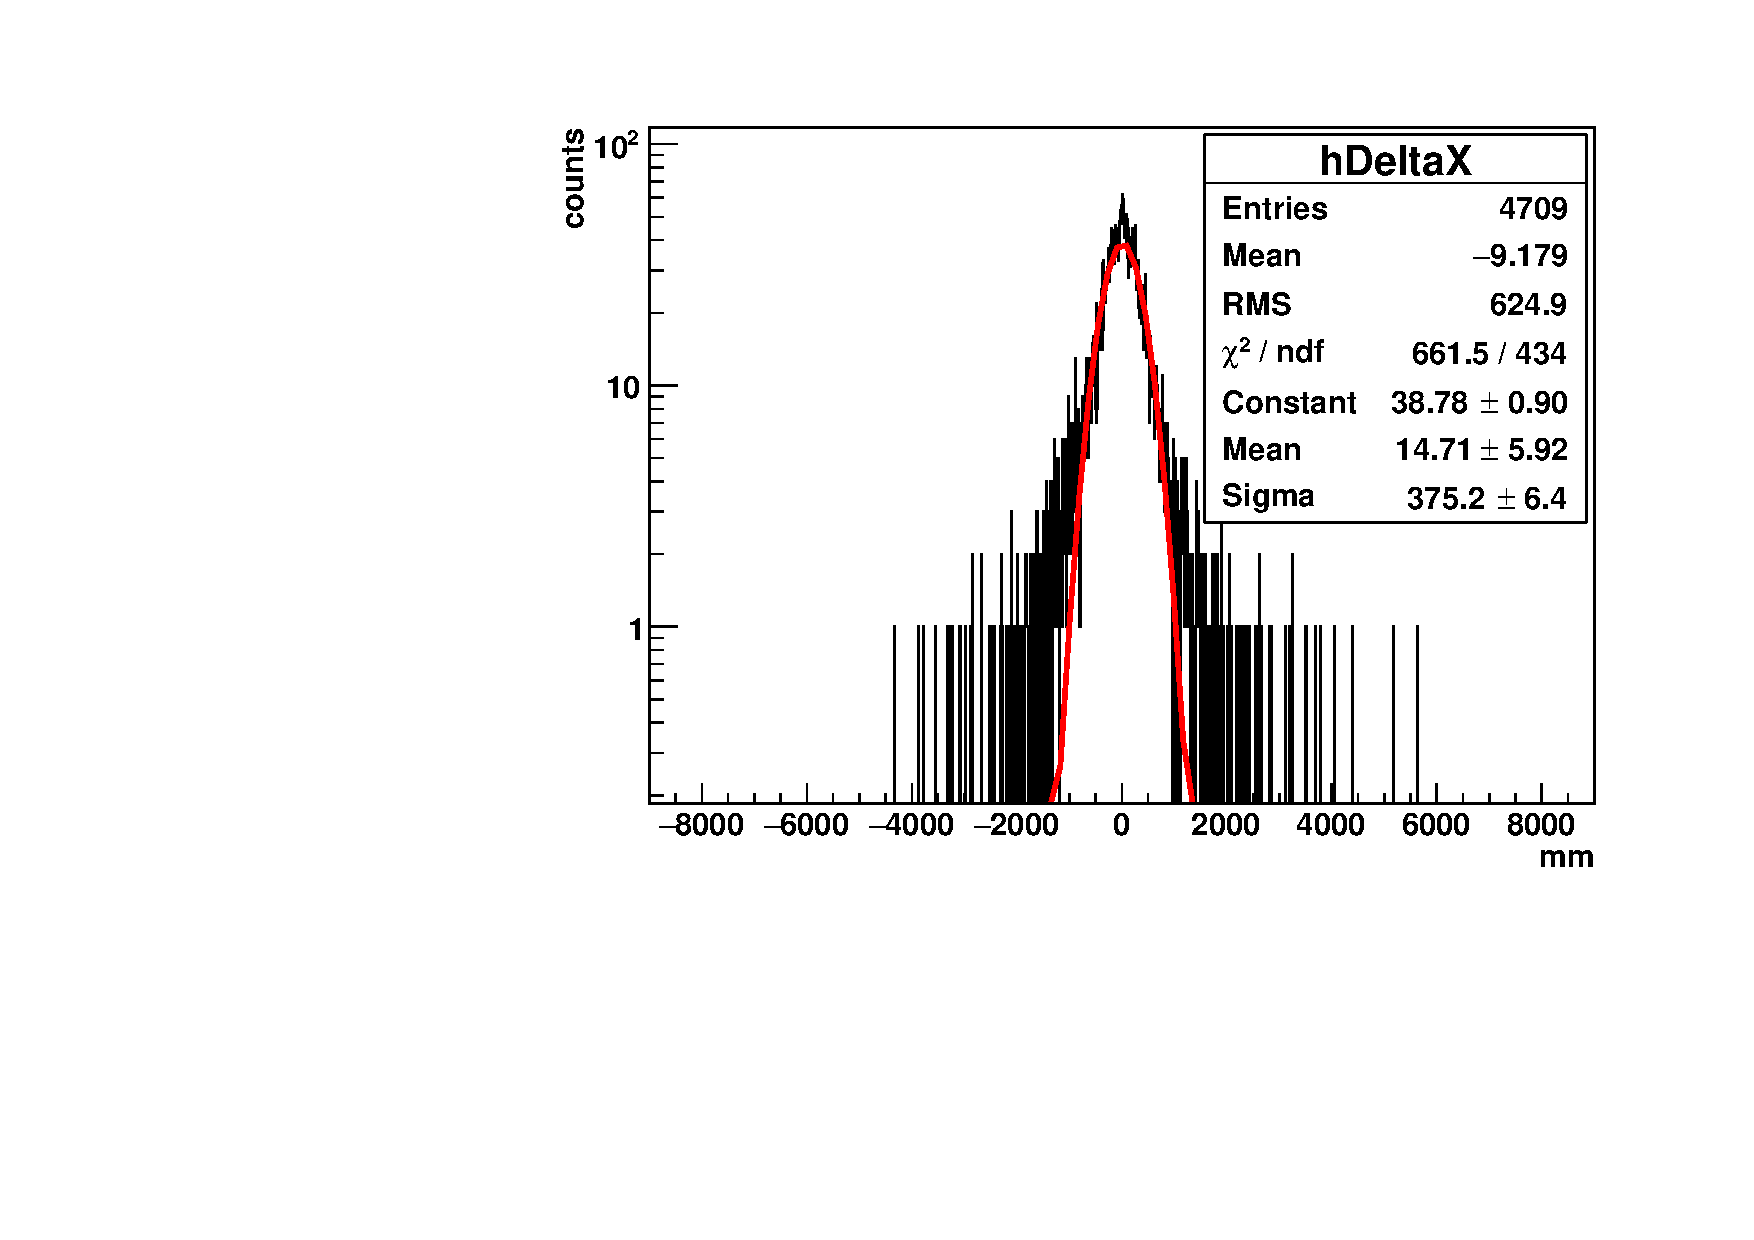
\includegraphics[width=6cm]{X_2p2MeVgamma.pdf}
		\end{minipage}
	}   
	\subfigure[$y_{fit}-y_{mc}$]{ 
		\begin{minipage}[t]{0.38\textwidth}
			\centering
			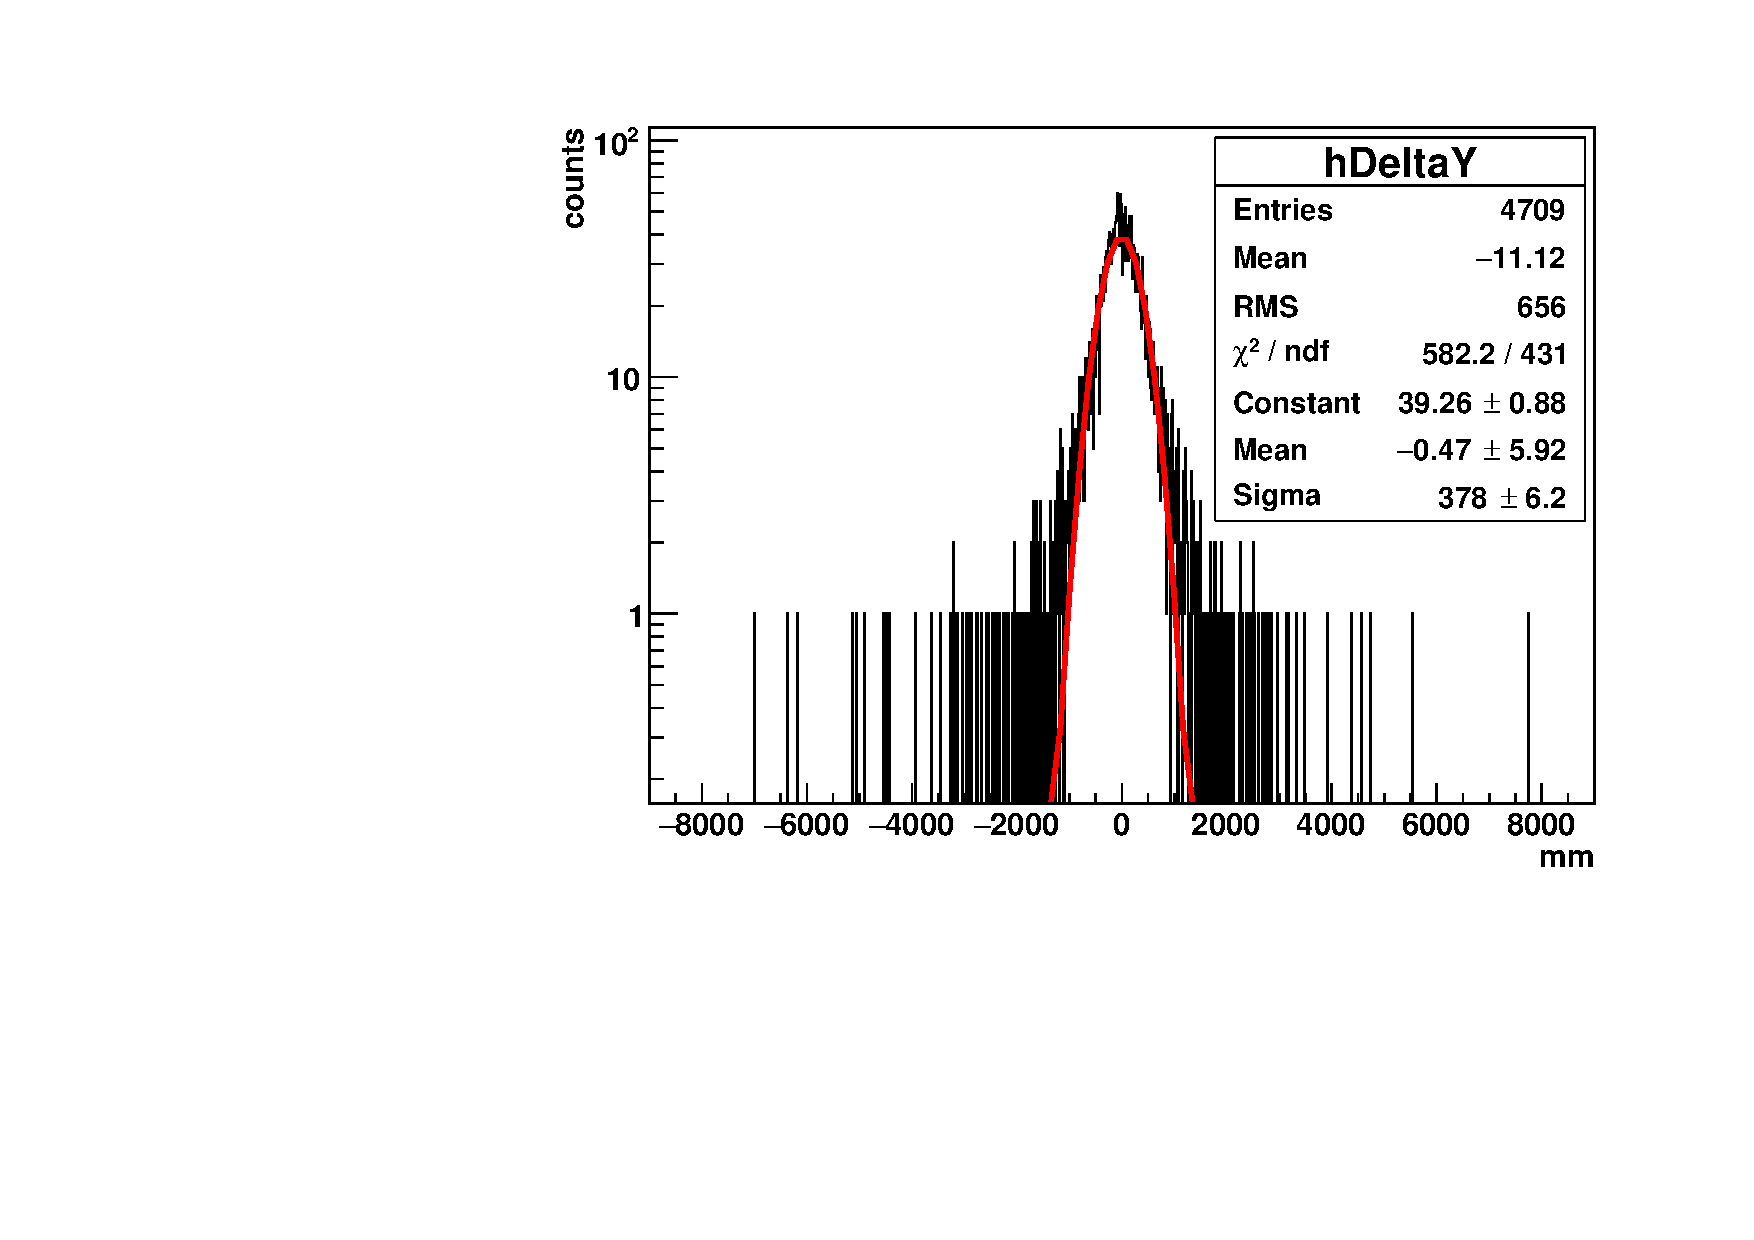
\includegraphics[width=6cm]{Y_2p2MeVgamma.pdf}
		\end{minipage}
	}
	\subfigure[$z_{fit}-z_{mc}$]{ 
		\begin{minipage}[b]{0.32\textwidth}
			\centering
			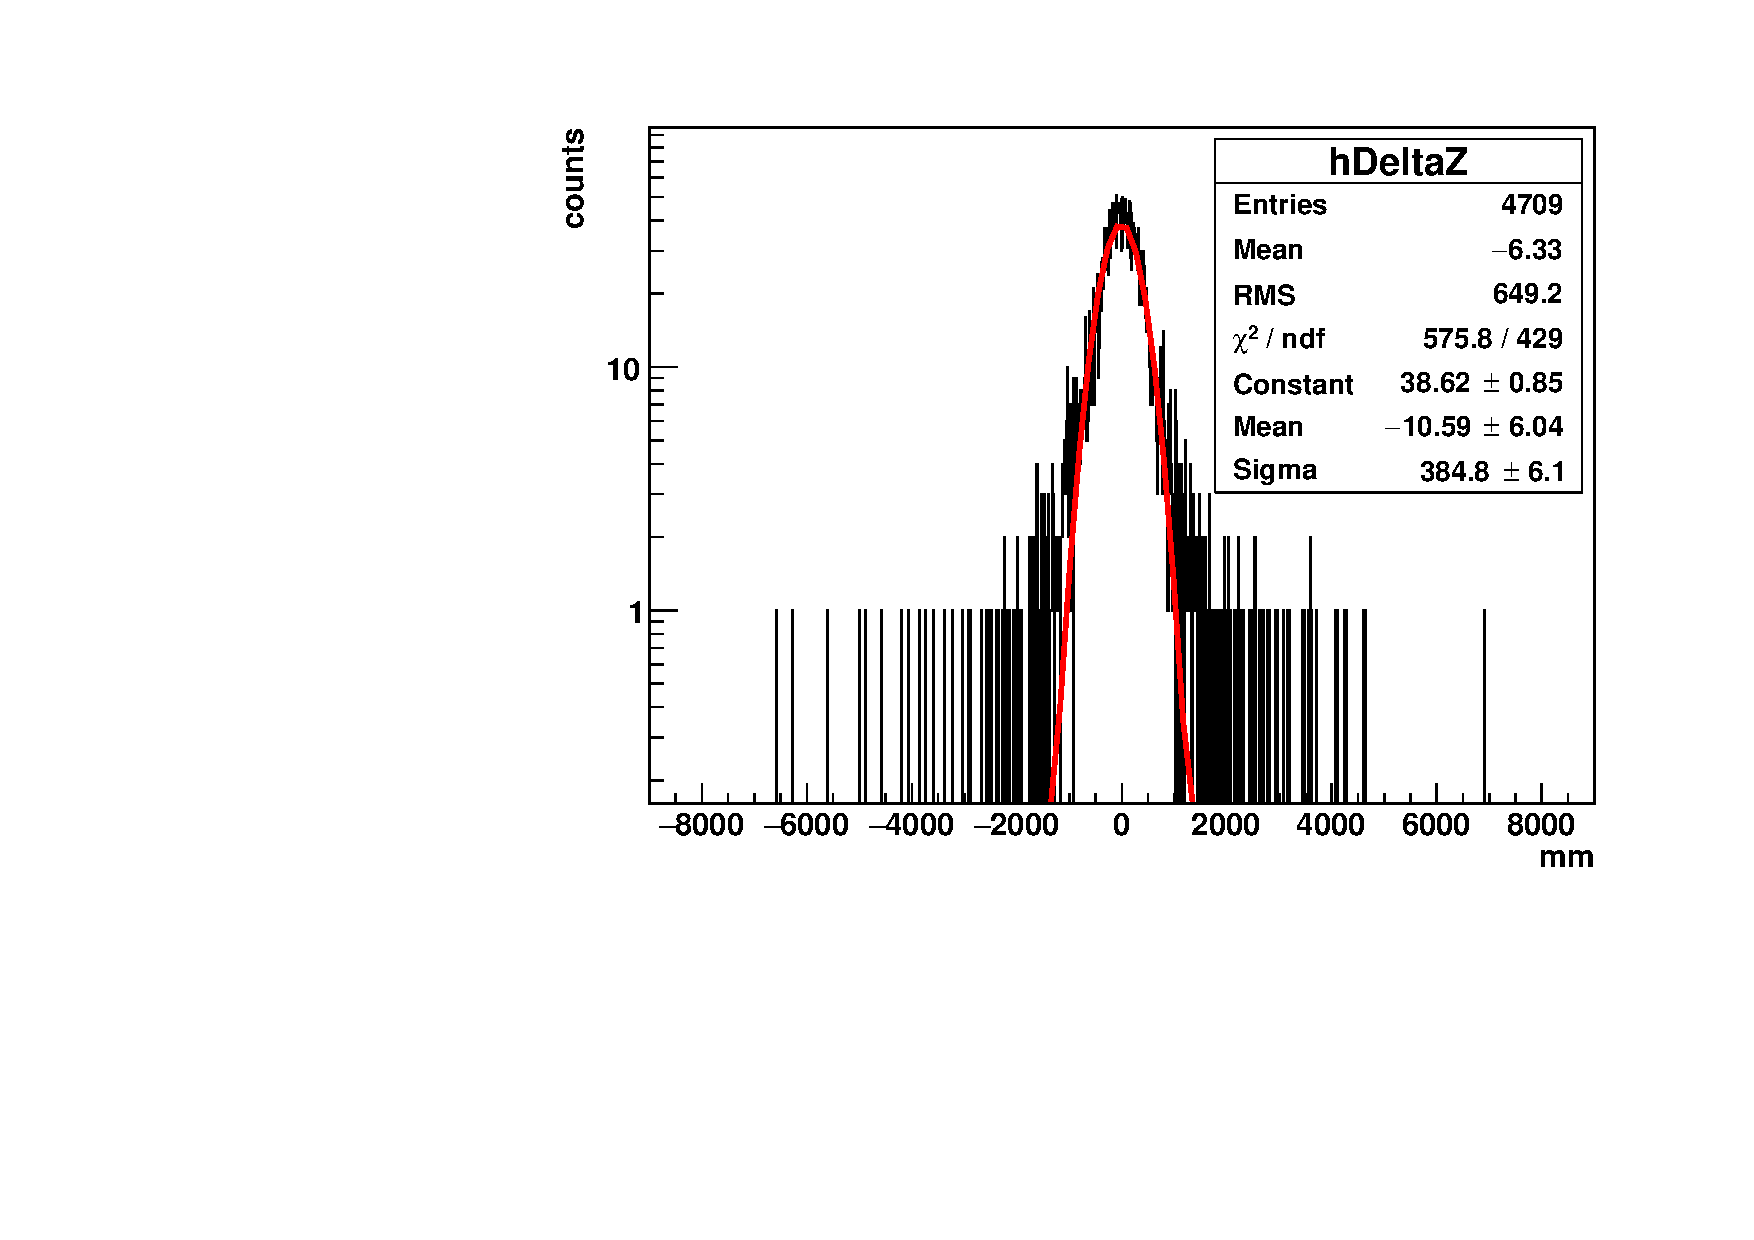
\includegraphics[width=6cm]{Z_2p2MeVgamma.pdf}
		\end{minipage}
	}
	\caption{Distributions of fit position bias projected on x axis ($\vec{X}_{fit}-\vec{X}_{MC}$) for $10^5$ MC simulations of 2.2 MeV $\gamma$ events.}
\end{figure}



4.4-MeV $\gamma$ events
\begin{figure}[htbp]
	\centering
	\subfigure[$x_{fit}-x_{mc}$]{
		\begin{minipage}[t]{0.38\textwidth}
			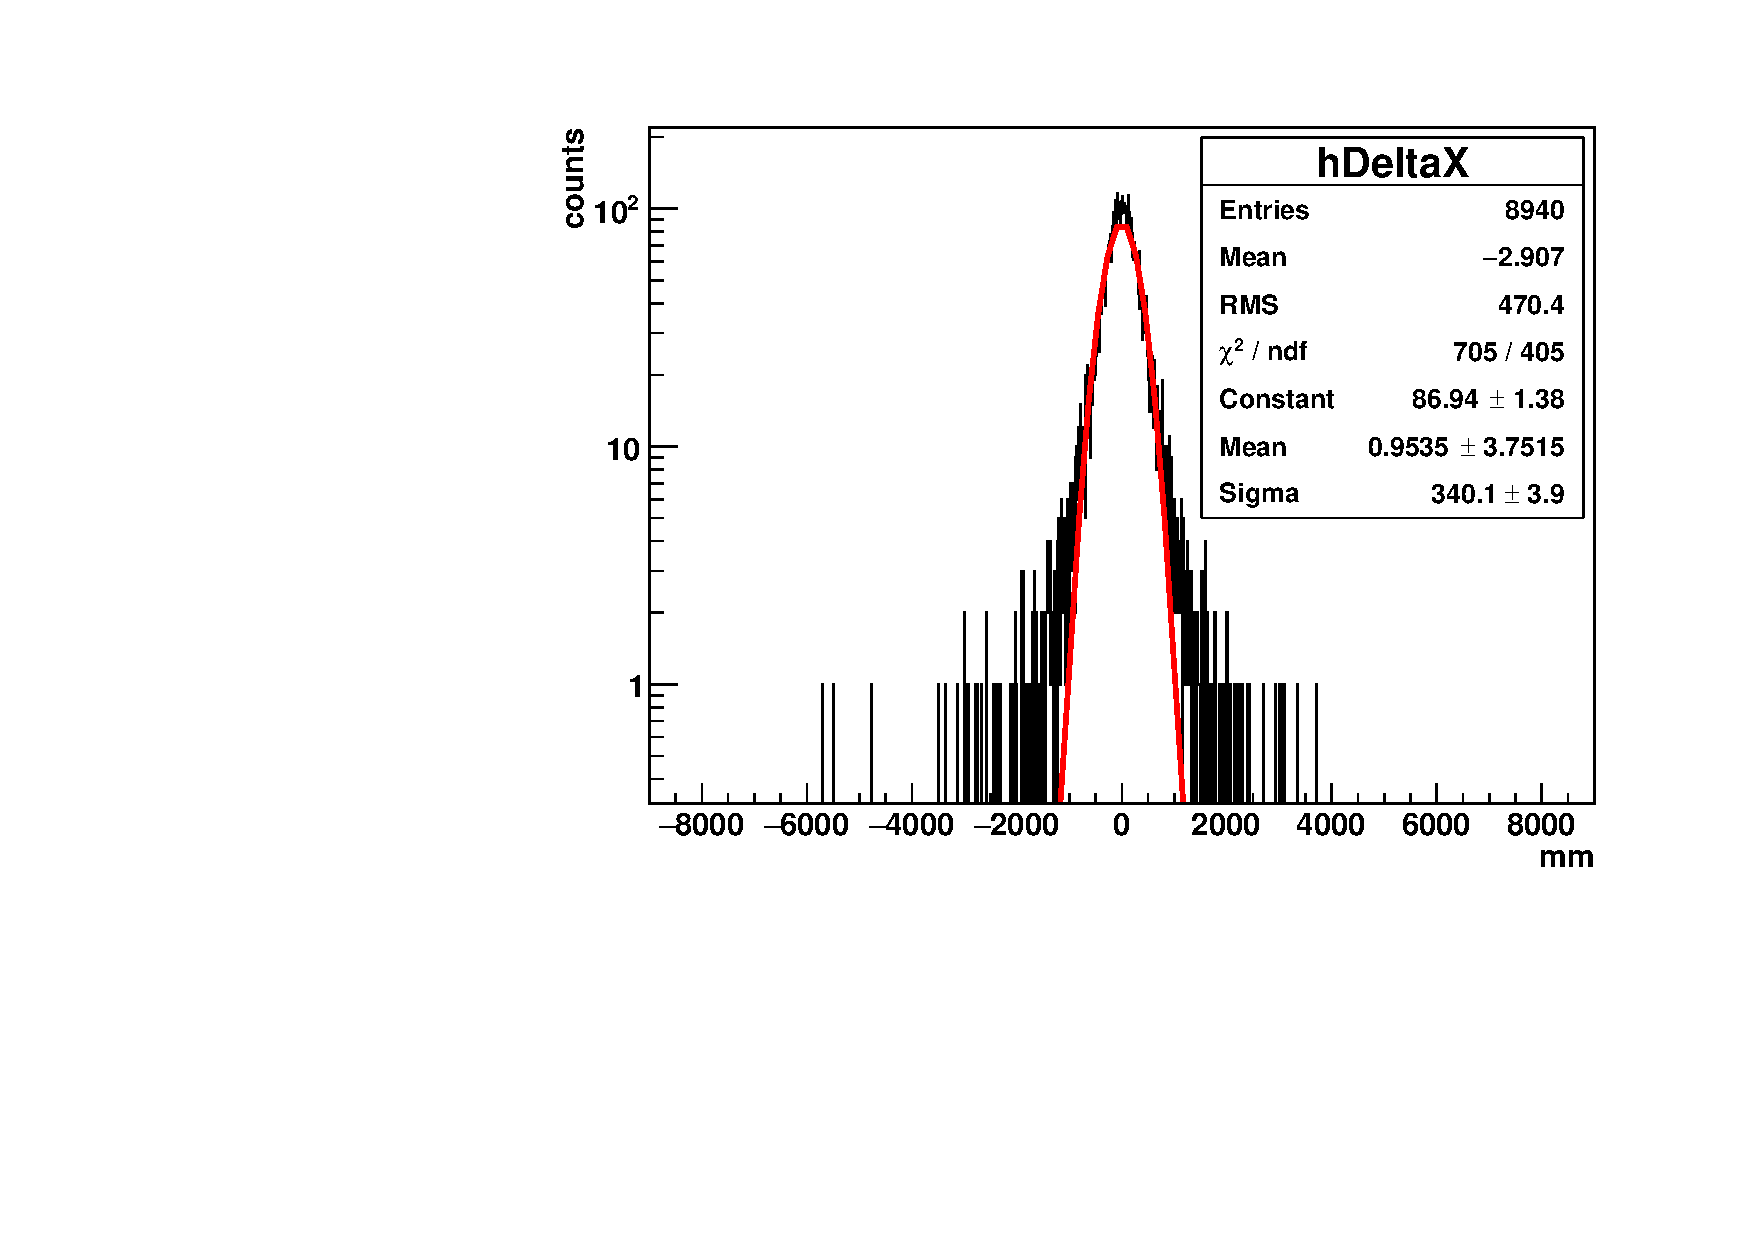
\includegraphics[width=6cm]{X_4p4MeVgamma.pdf}
		\end{minipage}
	}   
	\subfigure[$y_{fit}-y_{mc}$]{ 
		\begin{minipage}[t]{0.38\textwidth}
			\centering
			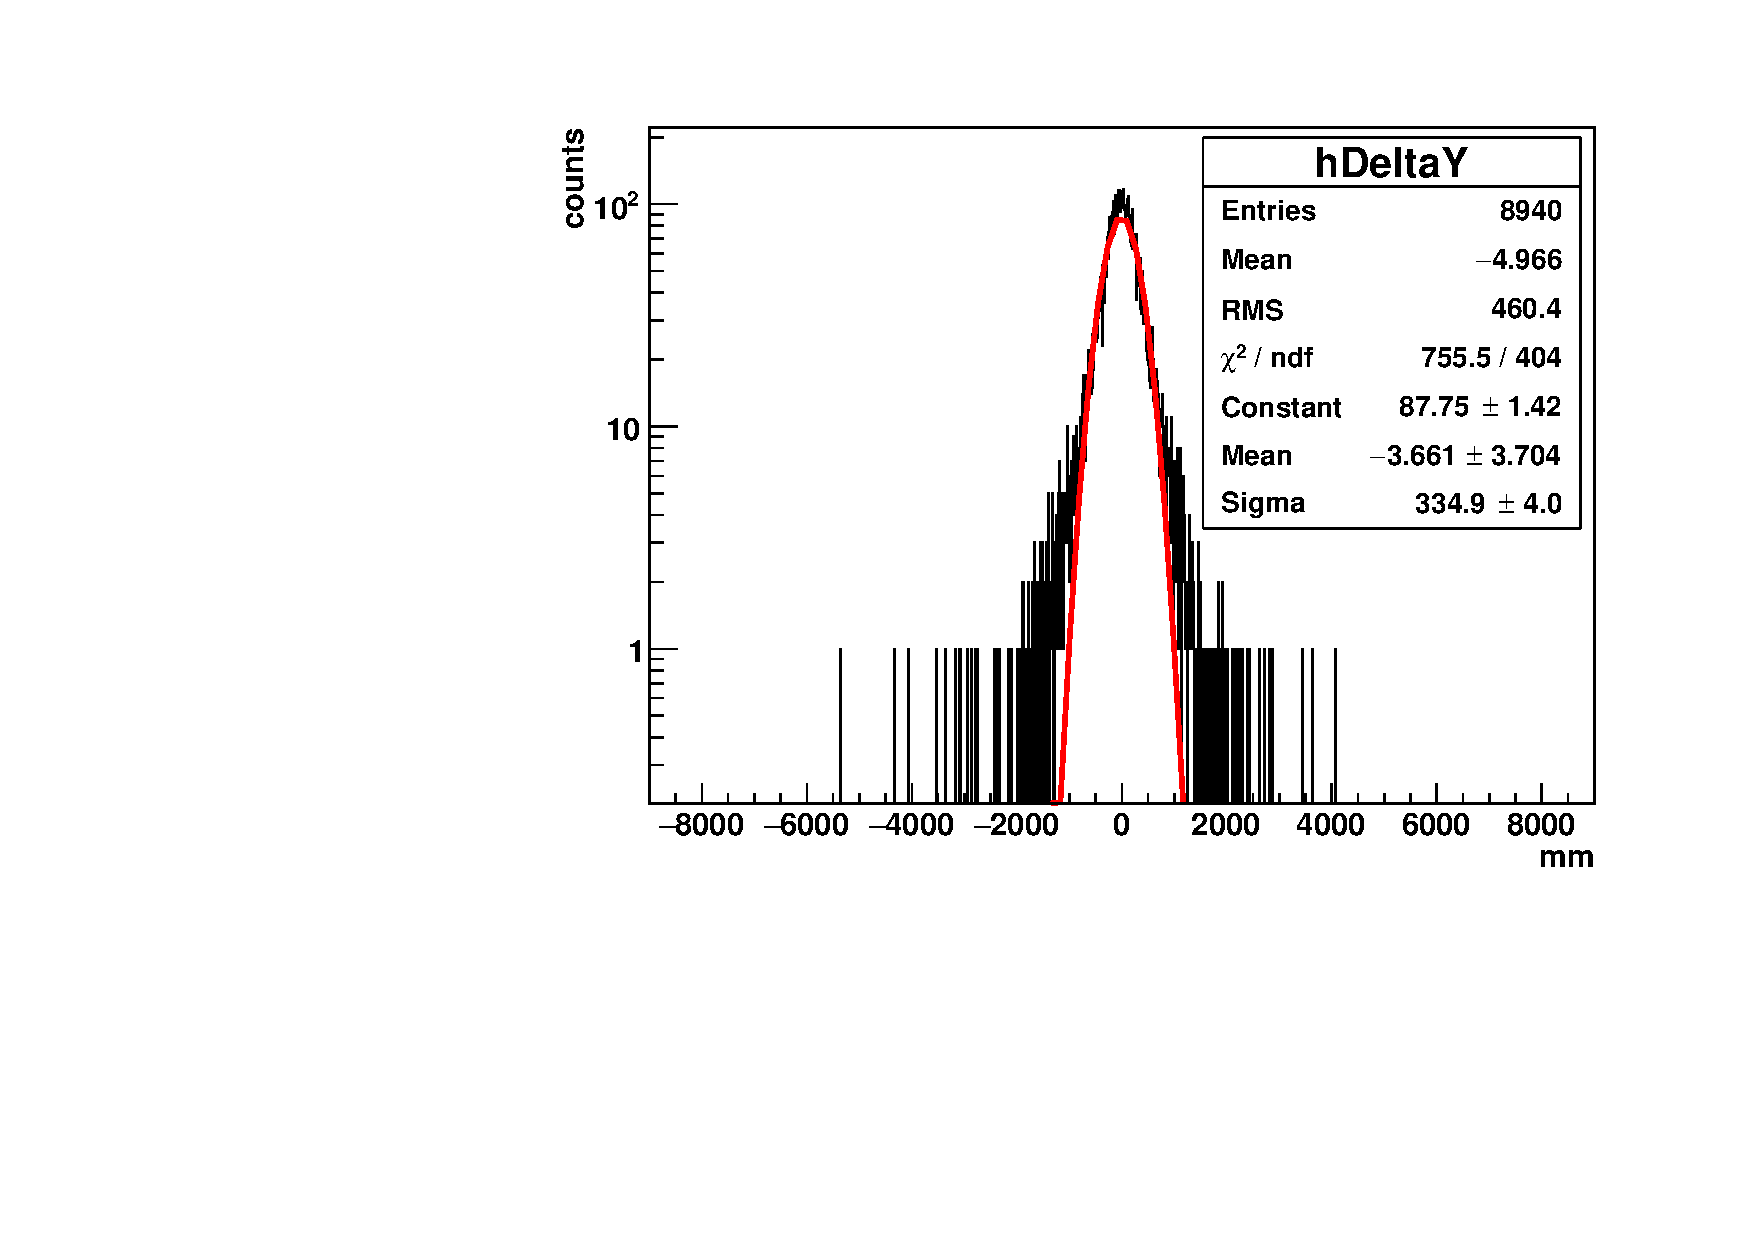
\includegraphics[width=6cm]{Y_4p4MeVgamma.pdf}
		\end{minipage}
	}
	\subfigure[$z_{fit}-z_{mc}$]{ 
		\begin{minipage}[b]{0.32\textwidth}
			\centering
			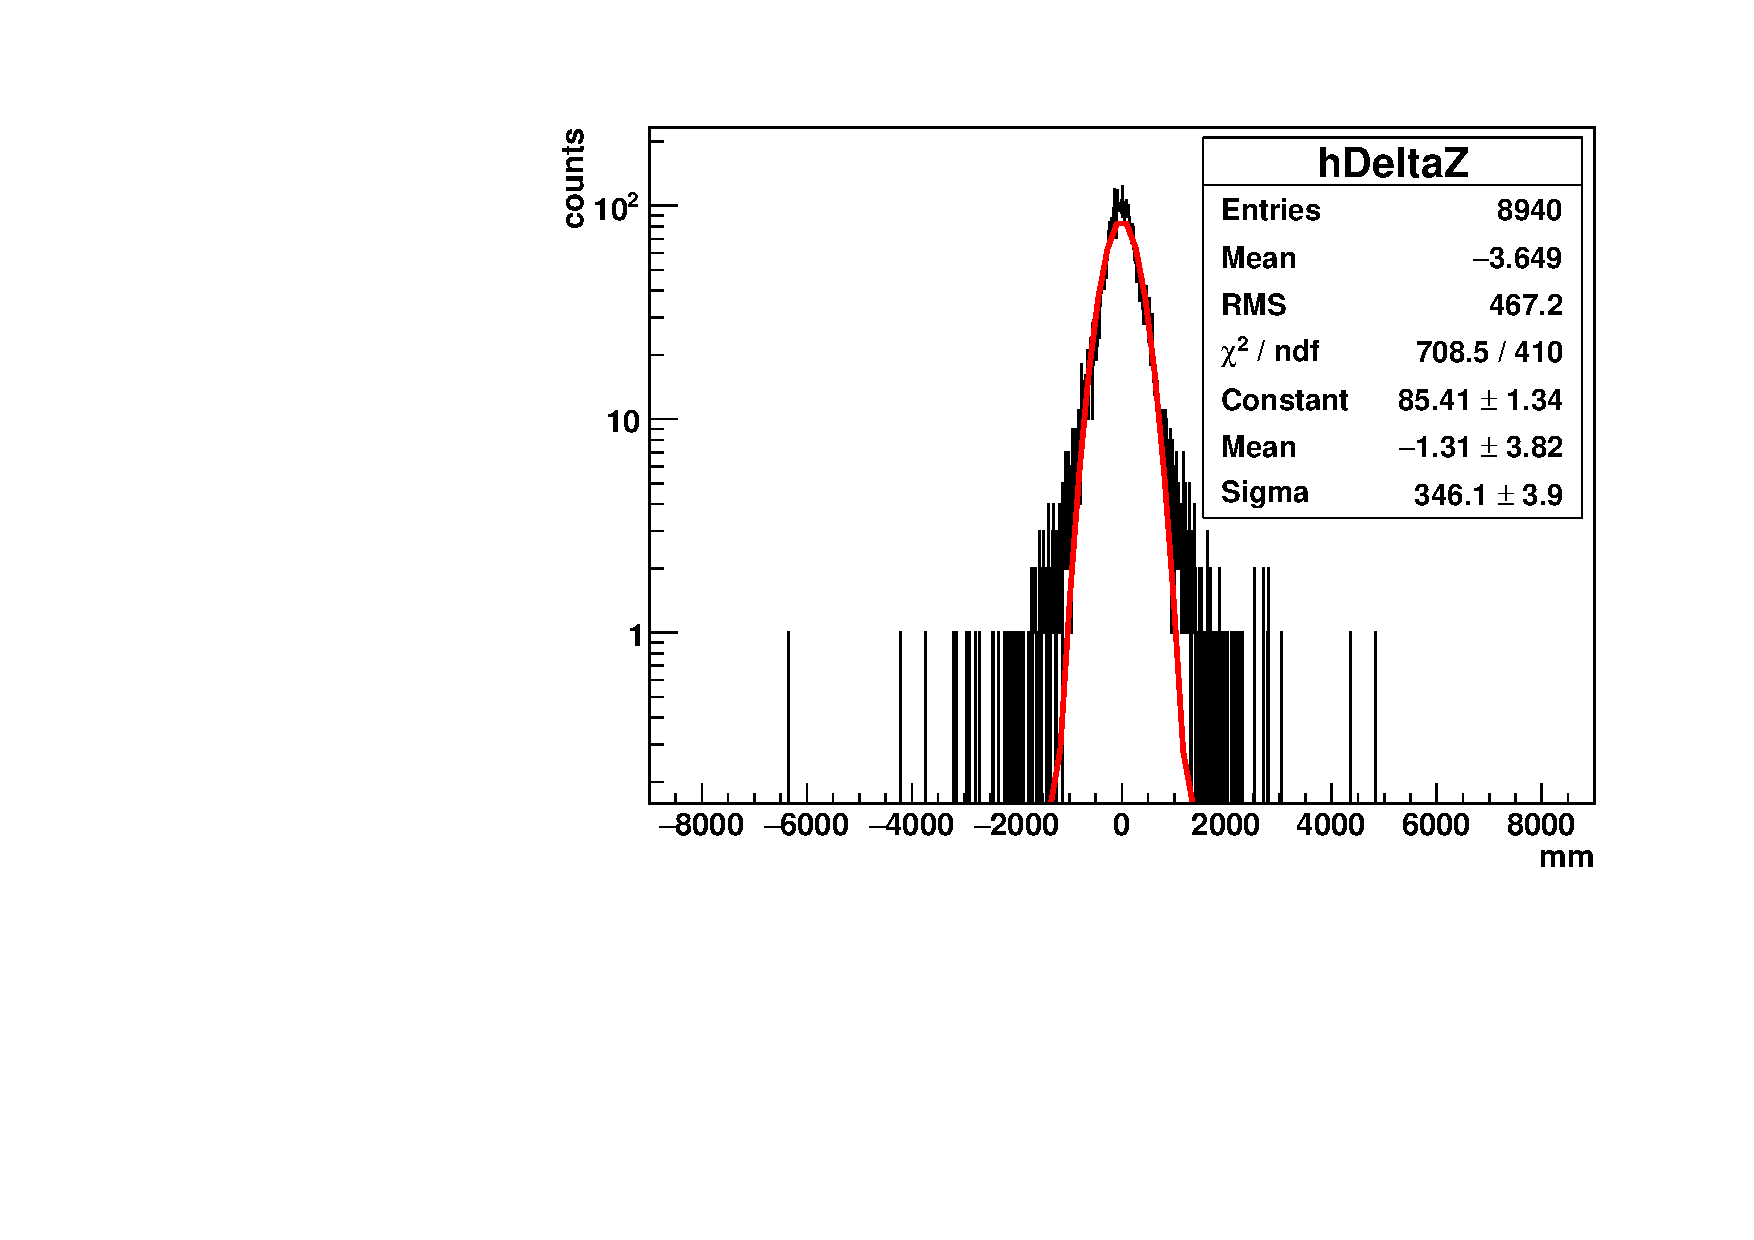
\includegraphics[width=6cm]{Z_4p4MeVgamma.pdf}
		\end{minipage}
	}
	\caption{Distributions of fit position bias projected on x axis ($x_{fit}-x_{MC}$) for 10000 MC simulations of 4.4 MeV $\gamma$ events.}
\end{figure}

\subsubsection{Test on $^{16}$N Calibration Source Events}
In a more realistic situation, the data collected from the runs of the calibration sources were used to evaluate the fitter performances as well as the reconstruction uncertainties. Chapter 5 will discuss the analyses of the $^{16}$N calibration source in detail. For these tests, a position resolution function including the distributions of the initial interaction positions, rather than the Gaussian function was used, while the same direction resolution function was used. 

\section{Vertex and Direction Reconstruction for the Water-based Wavelength-shifter}\label{sect:WLSfitter}
A reconstruction algorithm was developed to investigate the proposal for the water-based wavelength-shifter, as mentioned in \ref{sect:wbWLS}.

Figure~\ref{pmt_wls} shows the position distributions of hit PMTs for MC simulated 5 MeV electrons traveling along $+x$ direction in the AV. The left panel shows the case when the detector is filled with pure water while the right panel is for water plus 0.1 ppm PPO. For the same electrons, the number of hit PMTs ($\mathrm{NHits}$) in wbWLS is about 2.4 times greater than the pure water one. Although there is extra isotropic light emitted, the Cherenkov ring can still be seen clearly, allowing reconstruction of the directionality.  

\begin{figure}[htbp]
	\centering
	\begin{minipage}[t]{0.48\textwidth}
		\centering
		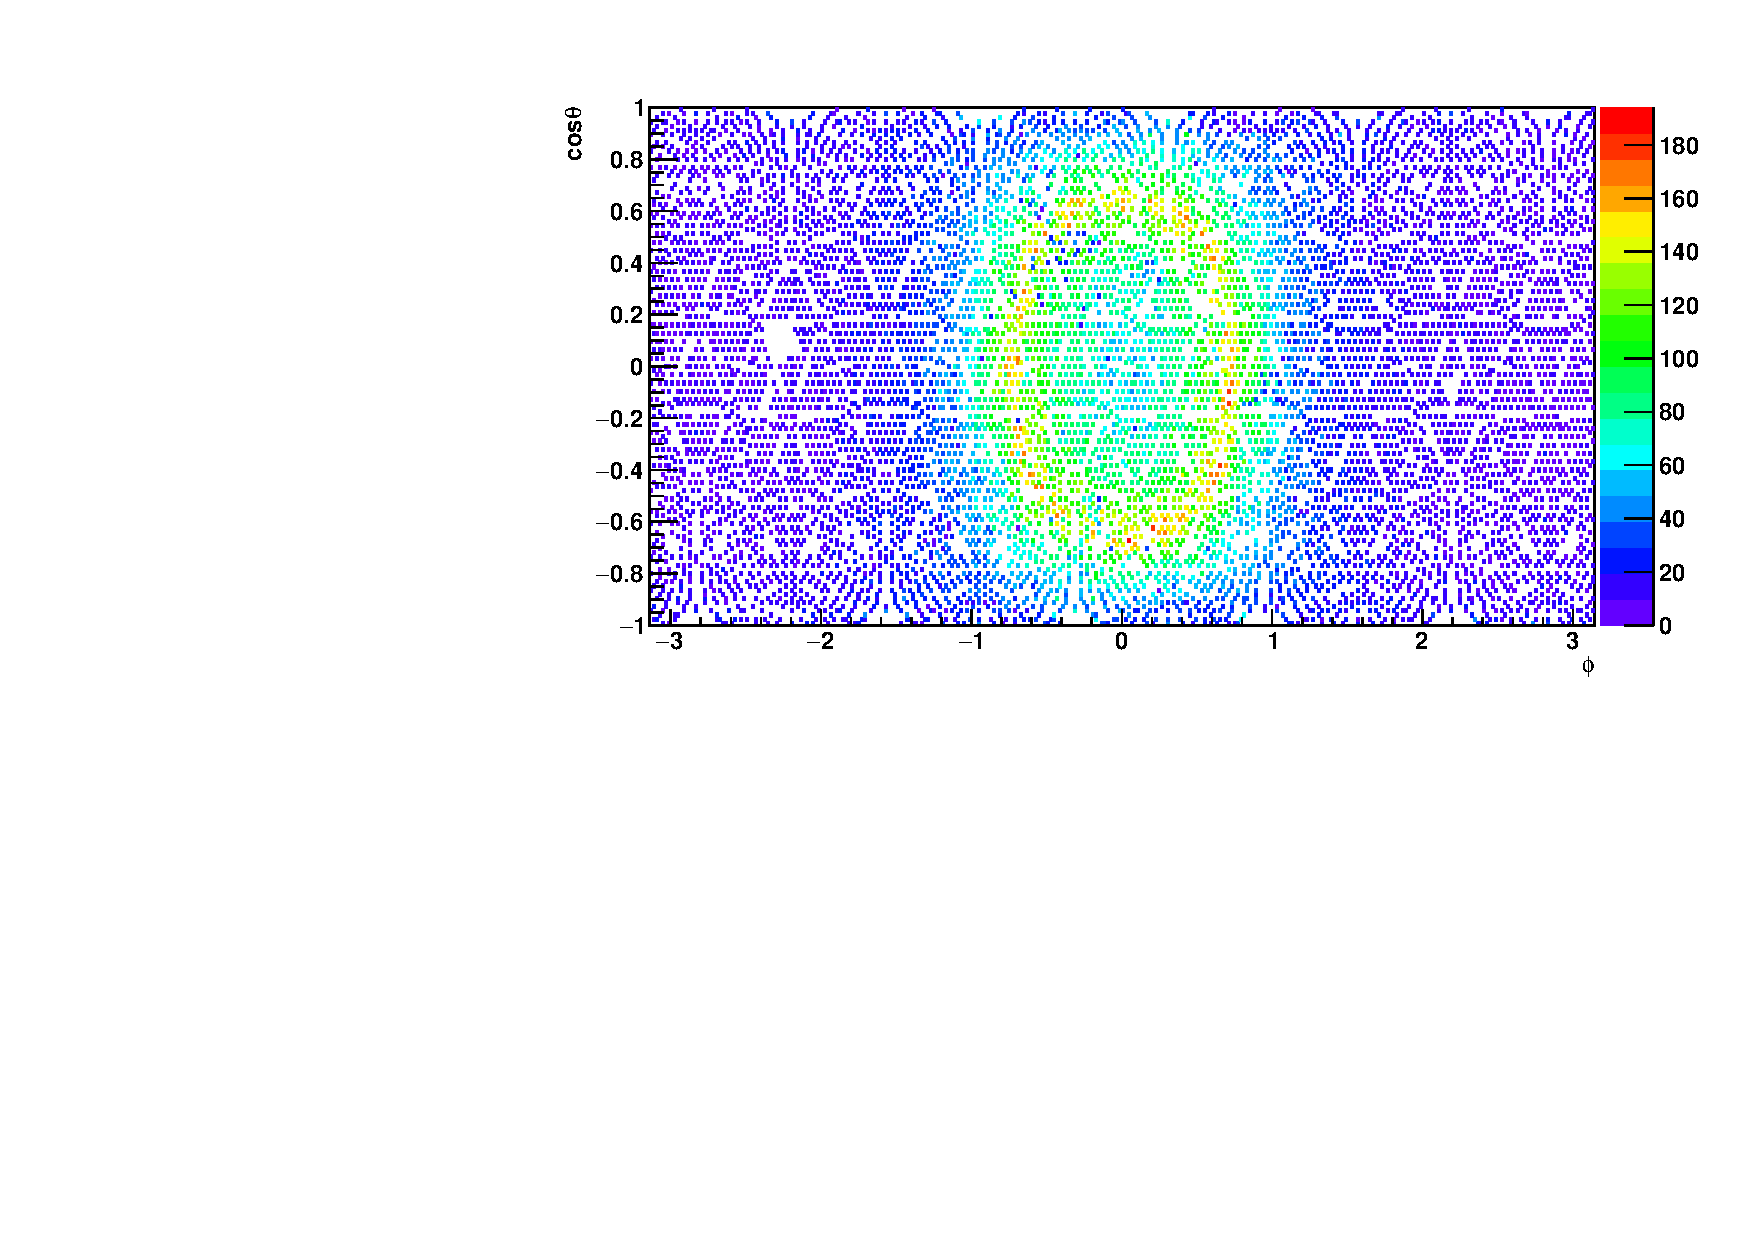
\includegraphics[width=7cm]{PMT_5MeVElectronWater.pdf}
	\end{minipage}
	\begin{minipage}[t]{0.48\textwidth}
		\centering
		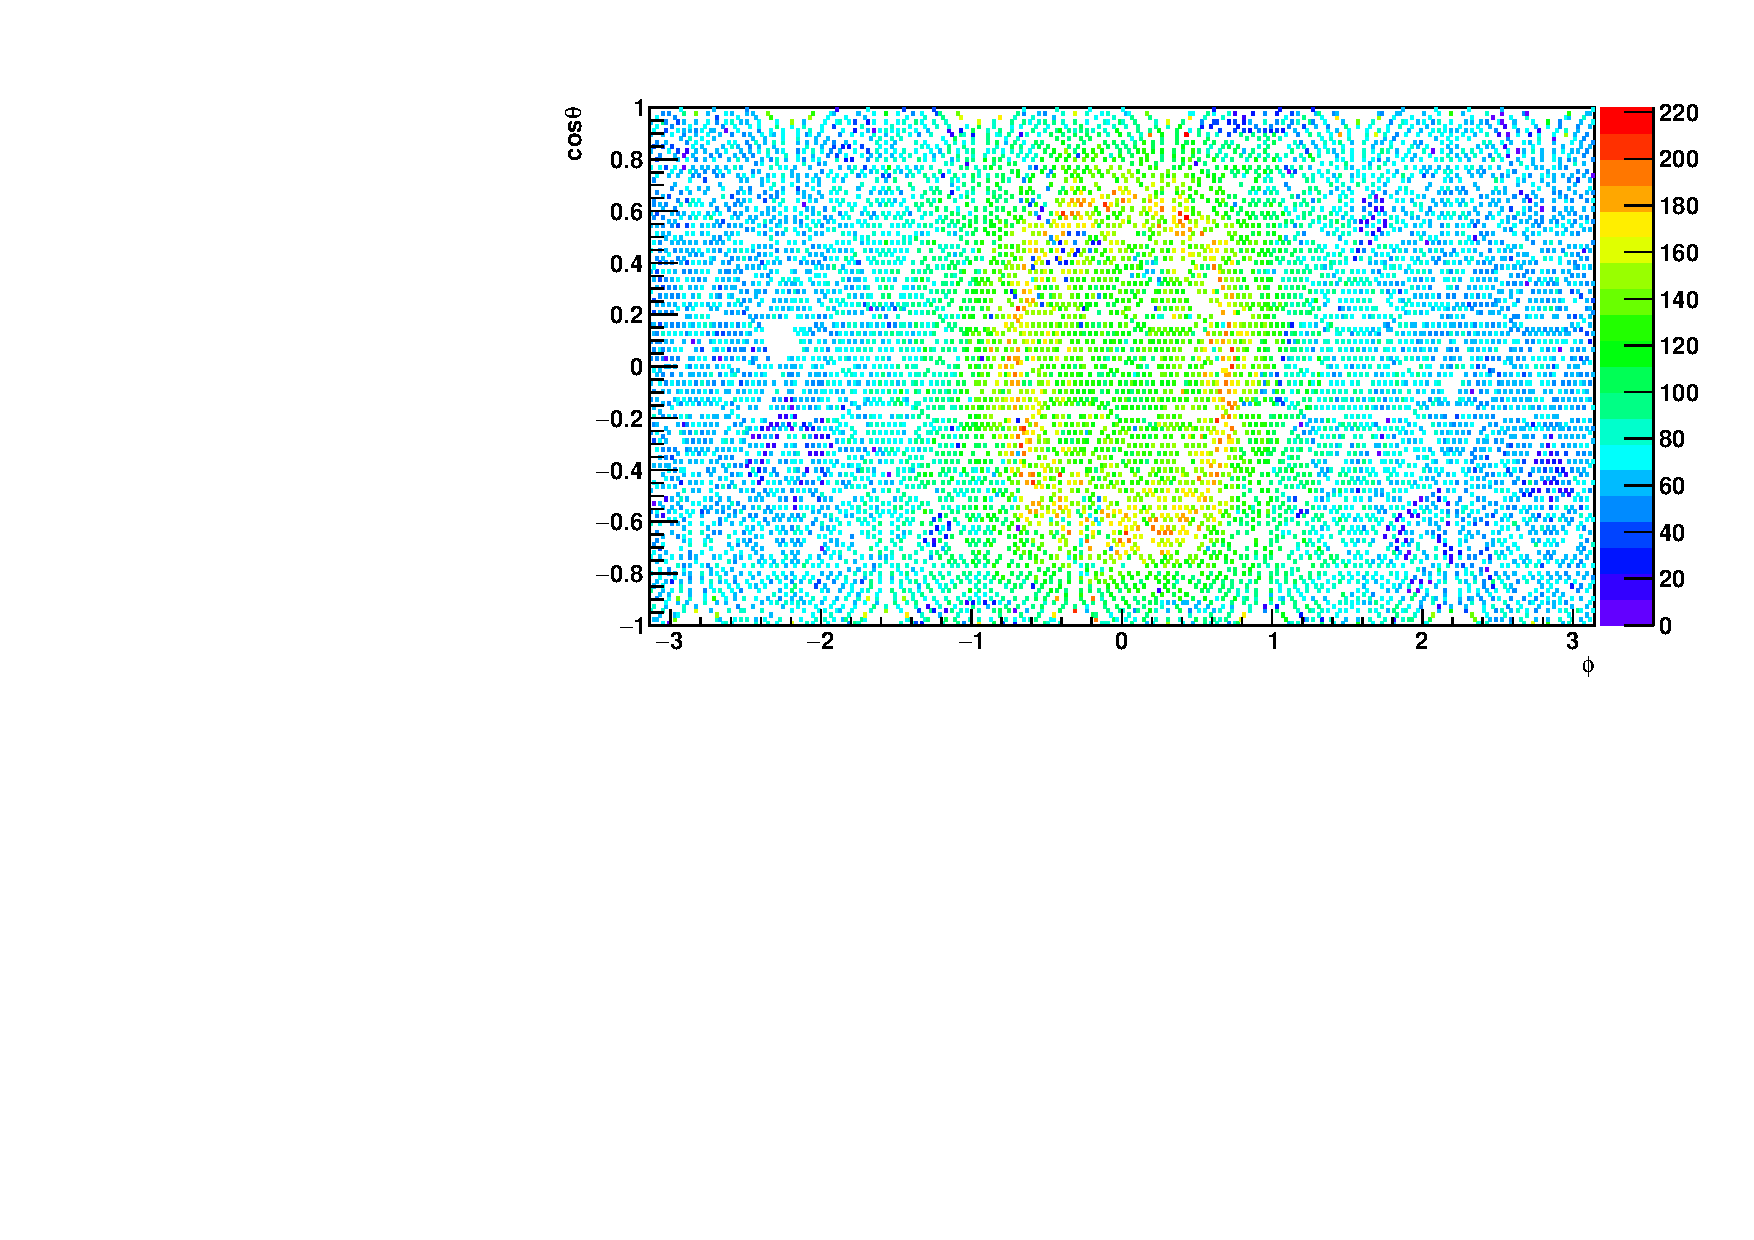
\includegraphics[width=7cm]{PMT_5MeVElectron0p1ppmPPO.pdf}
	\end{minipage}
	\caption{Position distributions of hit PMTs (in zenith and azimuth angles) for 5 MeV electrons traveling along $+x$ direction in the pure water (left) and the water plus 0.1 ppm PPO (right).}
	\label{pmt_wls}
\end{figure}

Figure~\ref{nhit_wls} shows the energies of simulated electrons as a function of the mean value of the $\mathrm{NHit}$ distribution (mean $\mathrm{NHits}$). In pure water, a 1 MeV electron simulation does not trigger any PMTs while in wbWLS case we have a mean $\mathrm{NHits}$ of 20.

\begin{figure}[htbp]
	\centering	
	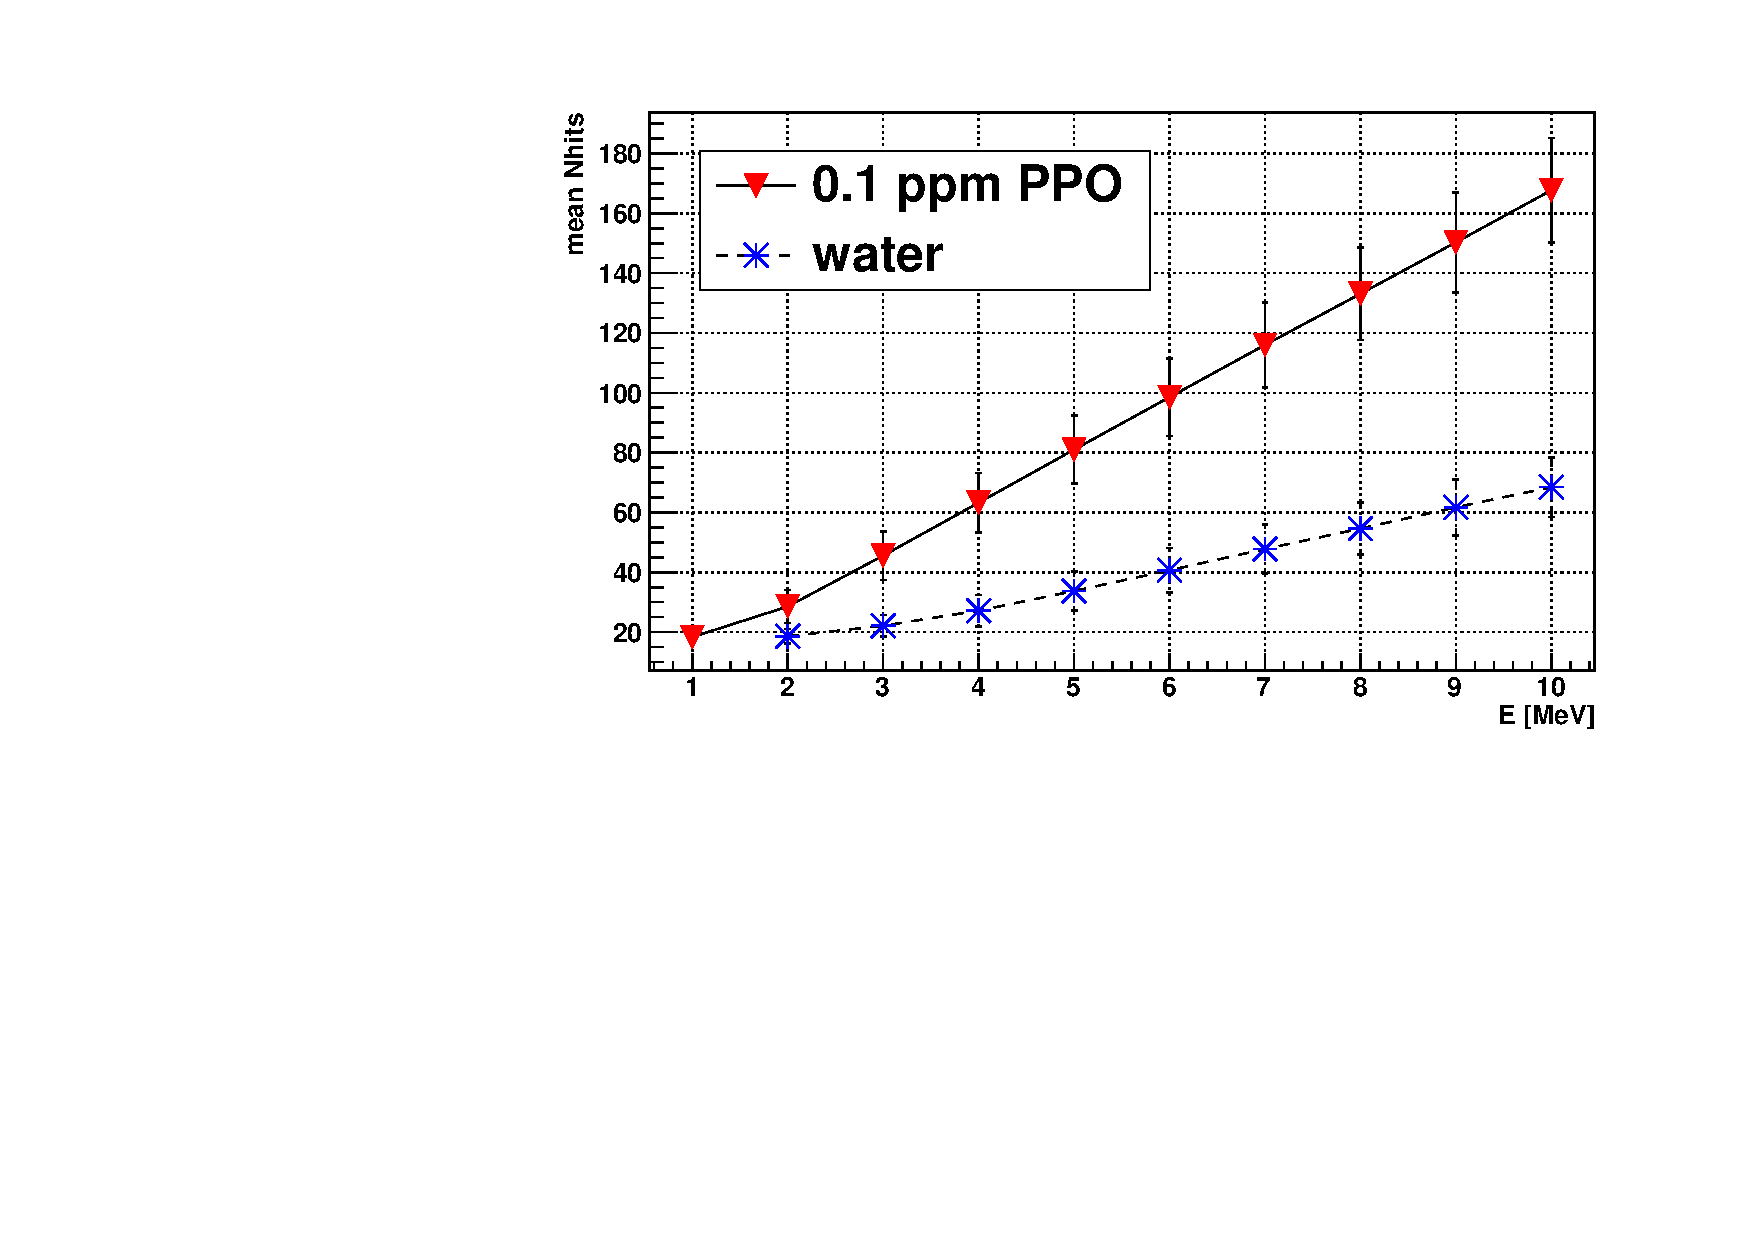
\includegraphics[width=9cm]{nhits_wls.pdf}
	\caption{ The energies of simulated electrons as a function of mean $\mathrm{NHits}$. The values in the 0.1 ppm PPO (solid line with inverted triangle) are compared with the water (dashed line with star).}
	\label{nhit_wls}
\end{figure}

In the wbWLS case, since WLS absorbs and re-emits photons, the reconstruction mentioned in section \ref{sect:mpw} is slightly modified to build the MP WLS Fitter. According to the optical property of PPO, the prompt light emitted from an event has a probability of $\sim$0.6 to be absorbed by the WLS and then re-emitted at a shifted vertex along the particle direction $\hat{n}$. Then the fitter returns a shifted vertex, $\vec{X}_{0,shifted}=\vec{X}_0+\mathrm{offset}\cdot\hat{n}$. The offset we set in the fitter is 100 mm obtained from simulations. Figure~\ref{WLS_pdf} shows the timing pdf for the wbWLS, which is the PMT response time modified to photon propagation time in the wbWLS.
\begin{figure}[htbp]	
	\centering		
	\begin{minipage}[b]{0.5\textwidth}			
		%\centering			
		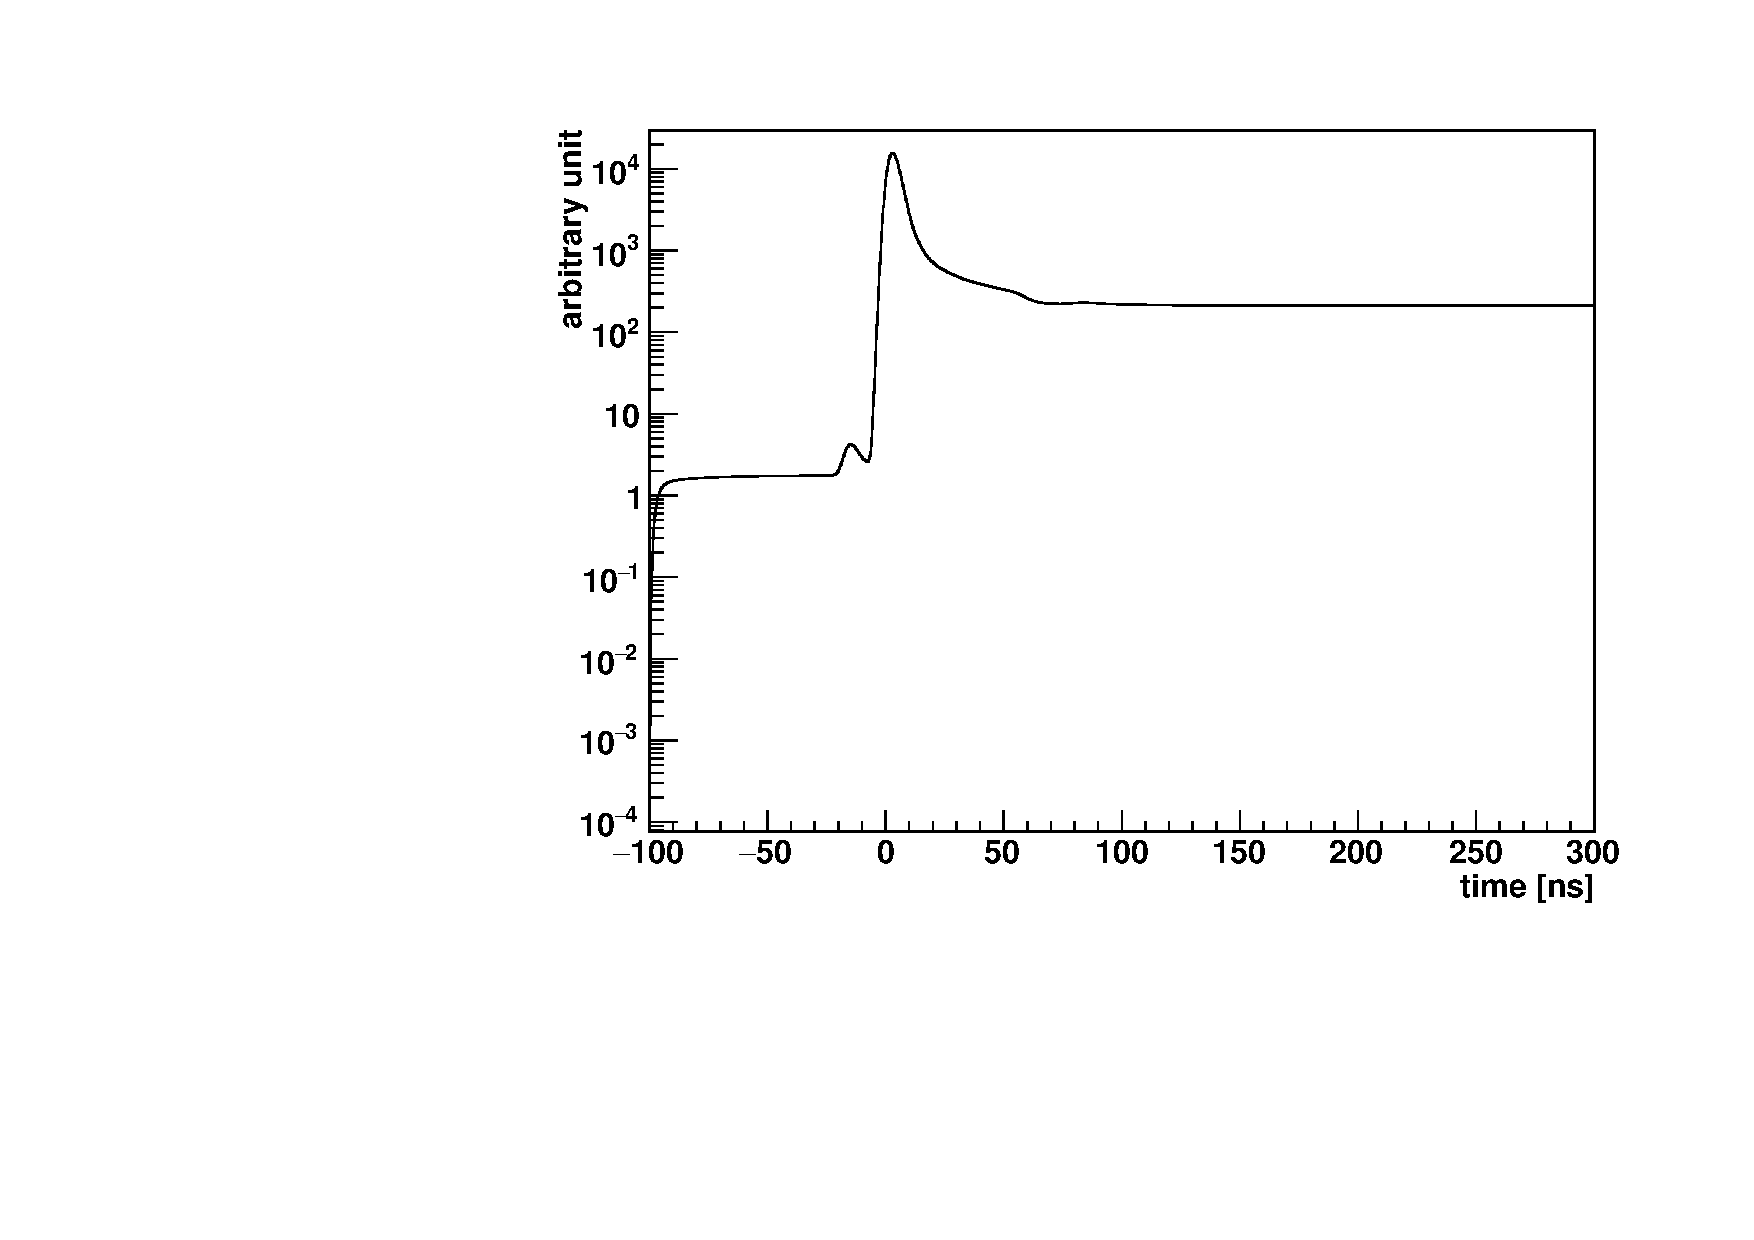
\includegraphics[height=6cm]{WLSTime_pdf.pdf}			
	\end{minipage}%				
%		\begin{minipage}[b]{0.5\textwidth}		
%			%\centering	
%			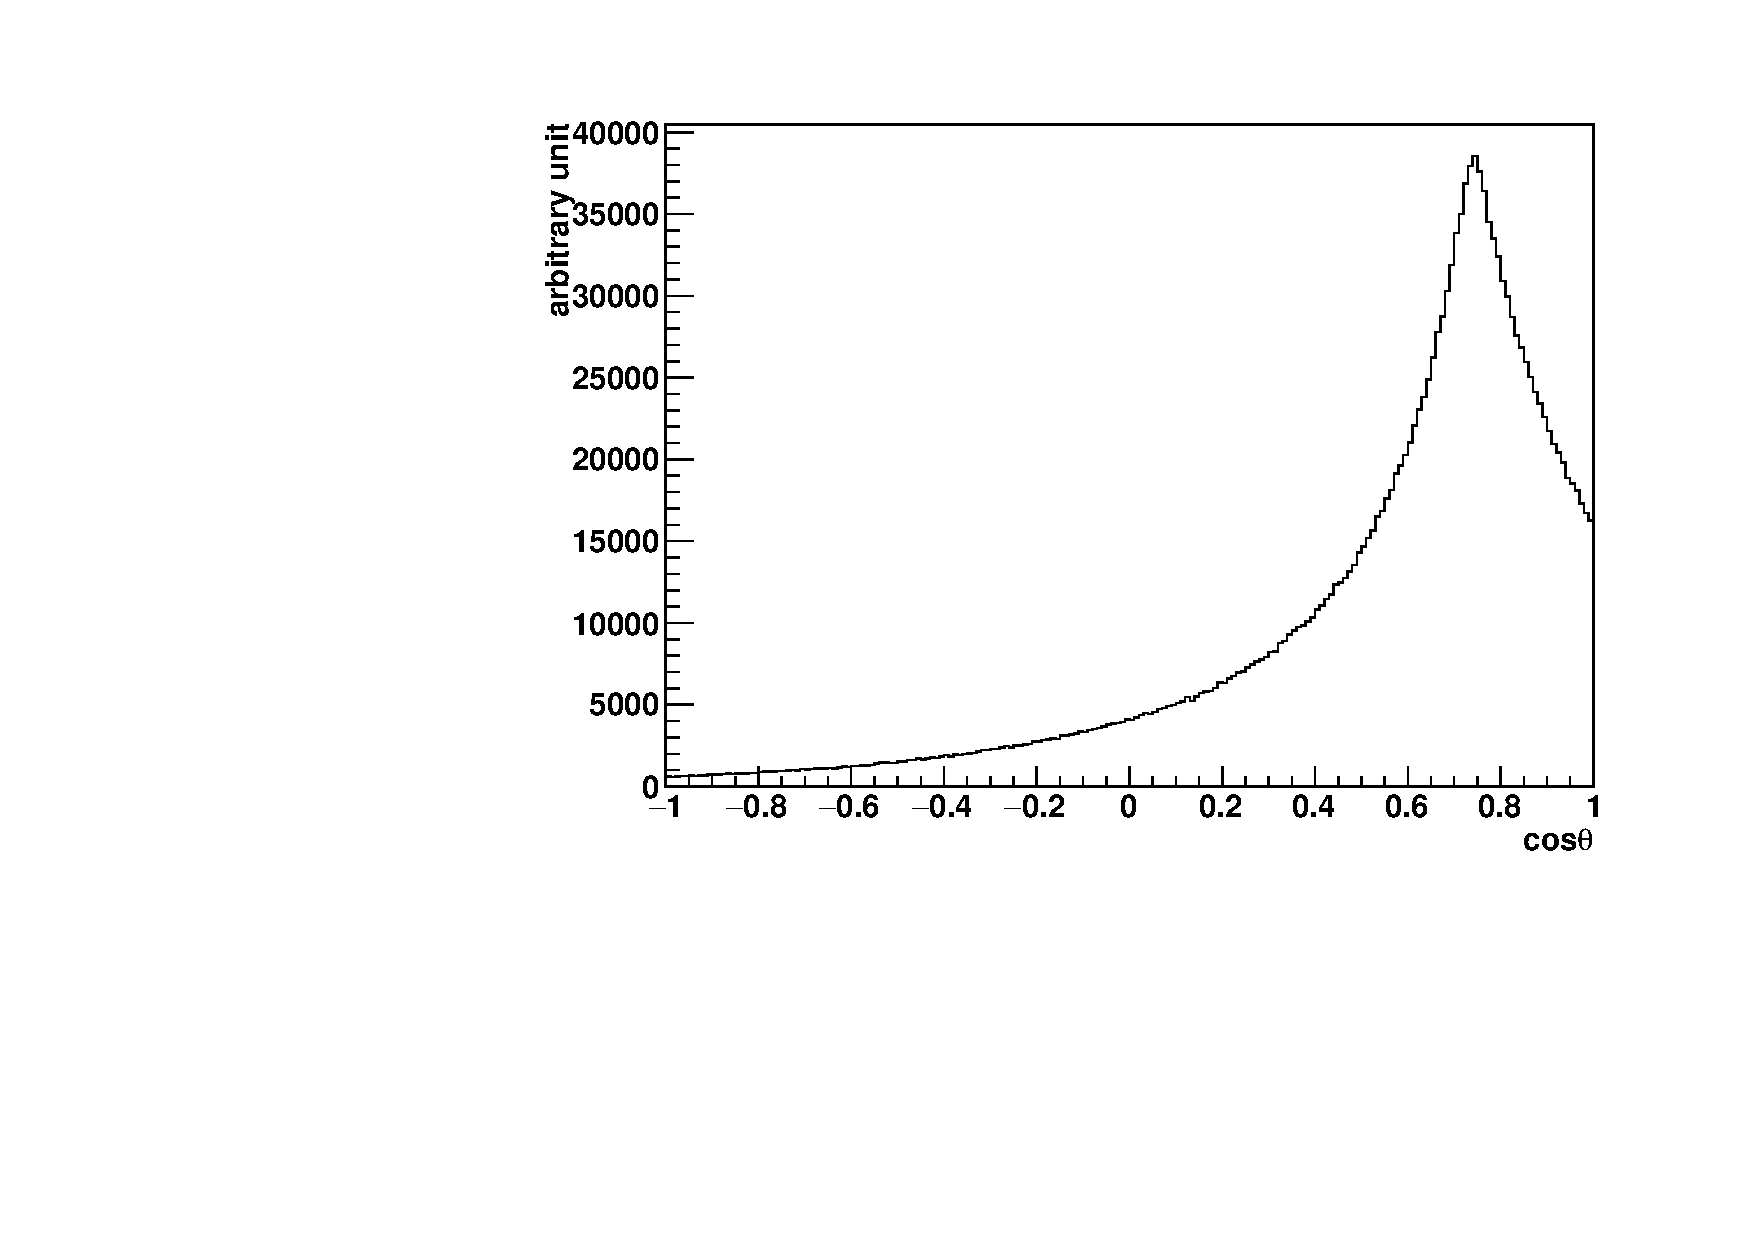
\includegraphics[height=5cm]{ChAngle_pdf.pdf}	
%		\end{minipage}	
	\caption{\label{WLS_pdf} The timing pdf for the wbWLS.}	
\end{figure}

To reconstruct the direction, besides the angular distribution of Cherenkov photons, $\cos\theta_{Ch}$, we also consider the fraction of the re-emitted and wavelength shifted photons that cause a flat angular distribution.

To test the performance of the \texttt{MP WLS Fitter}, 5 MeV electrons were simulated at the center of the AV filled with wbWLS and traveling along +x direction. As a comparison, the same simulation was done for the AV filled with pure water and the simulated events were reconstructed by the water fitter.

Fig.~\ref{WLSFitPos} shows the performance of the WLS fitter reconstructed positions of the MC simulations compared to the pure water case. For the fit position distribution of 5 MeV electrons in the wbWLS, we get a root mean square (RMS) of 201 mm and a bias to the center (the mean of histogram) of 29 mm. Compared to the pure water case, the fit bias is about 19 mm better and the RMS is 188 mm better.

\begin{figure}[htbp]	
	\centering			
	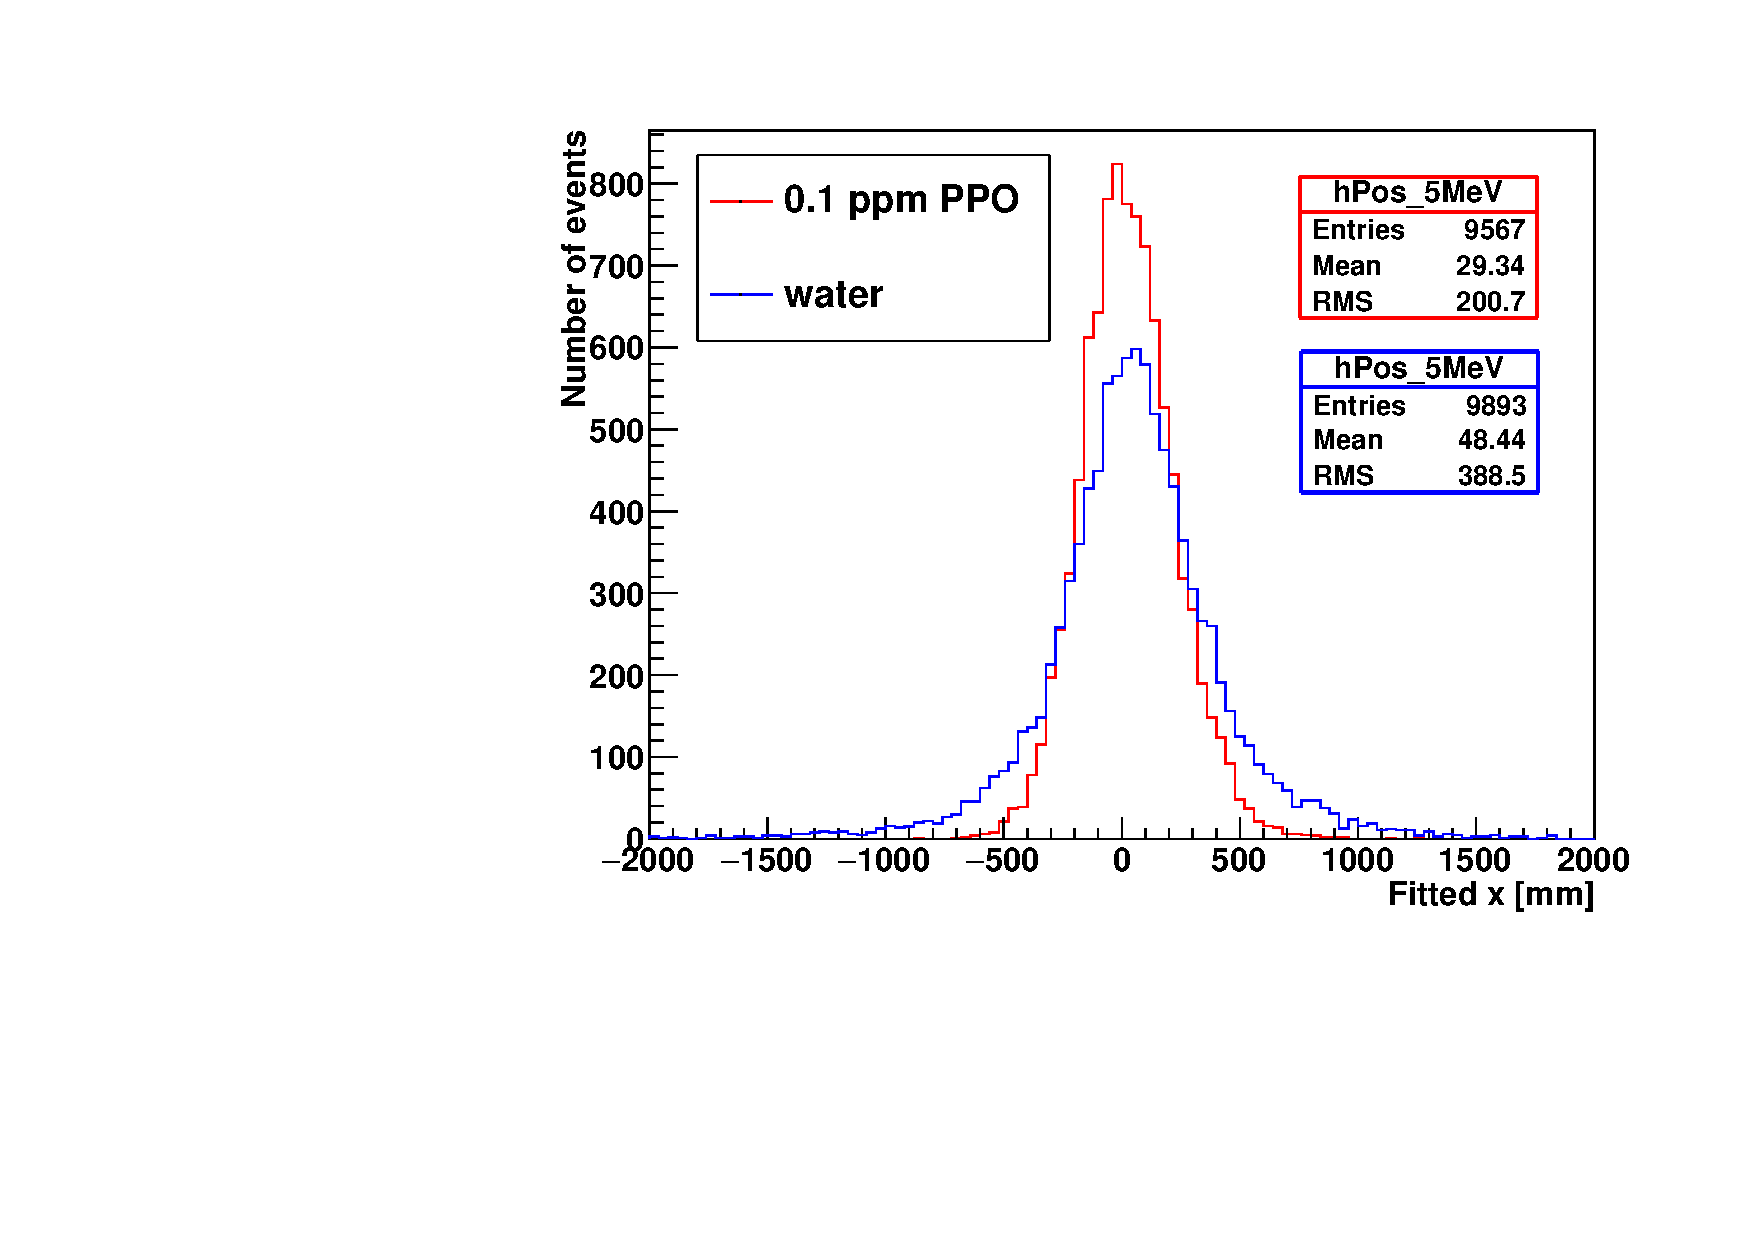
\includegraphics[height=5cm]{WLS_FittedPos.pdf}		
	\caption{\label{WLSFitPos} Fit position projected on x axis. The WLS fitter reconstructed $x$ positions of the 5 MeV electron events in the wbWLS (red) are compared to the ones in the water (blue).
	}
\end{figure}

For a given Cherenkov event, the error in the reconstructed event direction is defined as\cite{boulay2004direct}: $\cos(\theta_e)=\vec{u}_{fit}\cdot\vec{u}_e$, where $\vec{u}_e$ is the simulated electron direction and $\vec{u}_{fit}$ is the reconstructed direction. To quantify this error, we define a $\cos\theta_{a}$ so that:
\[
\frac{\int_{\cos\theta_{a}}^1 P(\cos\theta_e) d\cos\theta_e}{\int_0^1 P(\cos\theta_e) d\cos\theta_e} = a.
\] 
where $P(\cos\theta_e)$ is the distribution of $\cos\theta_e$ from MC data. The value of $\cos\theta_{a}$ is found numerically to let $\cos\theta_e$ contain $ a\cdot 100\%$ of the reconstructed data. A larger $\cos\theta_{a}$ means better direction reconstruction.

Table~\ref{quantAngular} shows the results of $\cos\theta_{a}$ for SNO heavy water data\cite{boulay2004direct} and simulations for SNO+ pure water and wbWLS. 

\begin{table}[ht]
	\caption{A comparison of quantitative estimates for the angular resolution between the SNO heavy water, SNO+ wbWLS and the SNO+ pure water cases.}\label{quantAngular}
				\centering		
		\begin{tabular*}{120mm}{c@{\extracolsep{\fill}}cccc}
			\toprule 
			medium & $\cos\theta_{0.9}$ & $\cos\theta_{0.8}$ & $\cos\theta_{0.5}$
			\\
			\midrule
			SNO heavy water  & 0.50 & 0.71 & 0.92  \\	
			SNO+ water  & 0.53 & 0.76 & 0.93	 \\
			wbWLS  & 0.37 & 0.63 & 0.90  \\	
			\bottomrule	
		\end{tabular*}
\end{table}

Comparing a pure water SNO+ detector and the wbWLS one, using the MP WLS Fitter for physics events gives a better position resolution without a significant loss in the performance of the direction reconstruction.

This fitter was tested for in \cite{mekarski2018electron}.

\section{Vertex Reconstruction for the Partial-fill}\label{sect:partialFitter}
The vertex reconstructions for the partial-fill and scintillator phases are very similar. Both of them treat two detection media: the water and the scintillator, and calculate the light paths in these two regions. I will first describe the calculations in the partial-fill case, since its geometry is more complicated while the full scintillator case can be considered as a simplified version.

\subsection{Partial-fill}

In the partial-fill geometry, the SNO+ detector can be described as a composition of three parts: the neck cylinder filled with the scintillator; the AV sphere, which is split by a water-scintillator interface (plane) inside, and above this plane is the scintillator and below is the water; and the PSUP sphere outside the neck and the AV, filled with the water.

Omitting the acrylic and other detector materials, photons mainly pass through two different media: the water and the scintillator. As shown in Fig.~\ref{fig:scintpath}, assuming a straight light path from a vertex to a hit PMT position, its total length is $|\vec{l}_p|=|\vec{X}_\mathrm{PMT}-\vec{X}_0|$. The \texttt{MP partial fitter} evaluates the length of the $|\vec{l}_p|$ in the scintillator: $d_{sp}$ and then the length in the water is $|\vec{l}_p|-d_{sp}$. Since photons travel at different speeds in these two media: $v_{gr,scint}$ and $v_{gr,water}$, the \texttt{MP partial fitter} evaluates the time of flight, $t_{transit}$ by:
\begin{equation}
t_{transit} = \frac{|\vec{l}_p|-d_{sp}}{v_{gr,water}} +\frac{d_{sp}}{v_{gr,scint}},
\end{equation}
and thus the time residual, $t_{res}$ is calculated. Once the $t_{res}$ is obtained, the following fitting procedure is the same to the \texttt{MP water fitter}.

\begin{figure}[!htb]
	\centering
	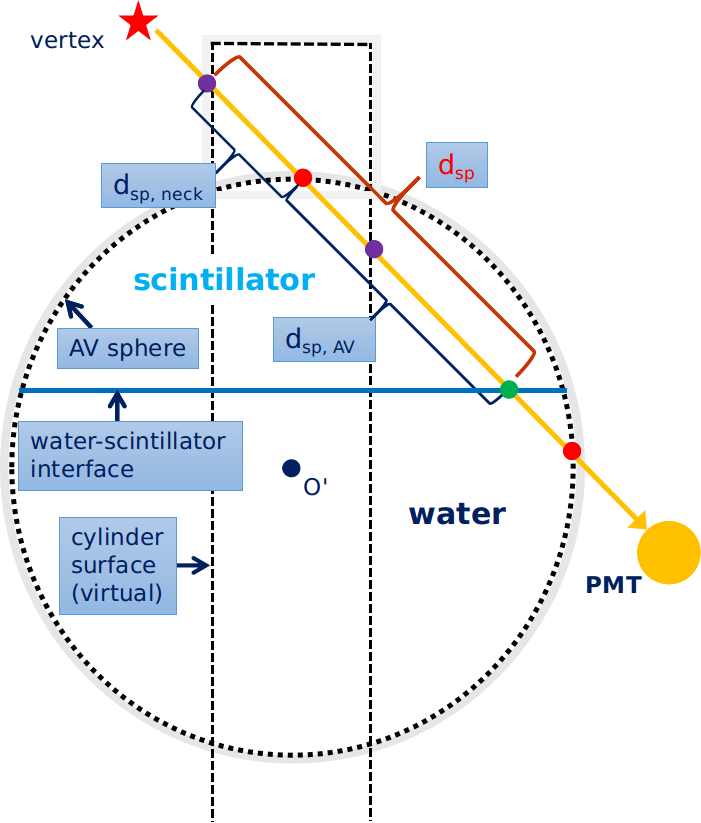
\includegraphics[width=7cm]{scintpath.png}
	\caption{Light path calculation for the \texttt{MP partial fitter}. In the figure, a light path intersects with the neck cylinder surface, the AV sphere as well as the water-scintillator interface. The total length of the path in the scintillator region (scintillator path, $d_{sp}$) includes the paths in the neck ($d_{sp,neck}$) and in the AV ($d_{sp,AV}$). Calculations of the ray-cylinder, ray-plane and ray-sphere intersections are applied.}
	\label{fig:scintpath}
\end{figure}

Therefore, the crucial part here is to calculate the $d_{sp}$. The light path $\vec{l}_p$ is considered as a ray with a direction (rather than a line without direction). The ray intersects with three geometry objects: the neck cylinder, the AV sphere and the water-scintillator interface plane. As illustrated in Fig.~\ref{fig:scintpath}, a detailed calculation of $d_{sp}$ includes the evaluations of (1) $\vec{l}_p$ and neck (ray-cylinder) intersection; (2) $\vec{l}_p$ and the AV (ray-sphere) intersection and (3) $\vec{l}_p$ and the water-scintillator interface (ray-plane) intersection. The $d_{sp}$ is further separated into the path lengths in the neck ($d_{sp,neck}$) and in the AV ($d_{sp,AV}$). 

For a trial position $\vec{X}_0=(x_0,y_0,z_0)$ and a hit PMT position $\vec{X}_{\mathrm{pmt}}=(x_\mathrm{pmt},y_\mathrm{pmt},z_\mathrm{pmt})$, define the ray vector as $\vec{l}_0\equiv\vec{X}_0+a\cdot \vec{u}$, where $a$ is the distance between vertex and intersection point and it is the parameter to be determined; $\vec u=\frac{\vec{X}_{\mathrm{pmt}}-\vec{X}_0}{|\vec{X}_{\mathrm{pmt}}-\vec{X}_0|}$ is the direction of the ray vector. It is a unit vector pointing from the $\vec{X}_0$ to the $\vec{X}_{\mathrm{pmt}}$. The following goes through the three intersection cases:

\begin{itemize}
\item Ray-sphere intersection

In the ray-sphere intersection case (ray vector passes through the AV sphere), the intersection points on the $\vec{l}_0$ satisfy the sphere equation $(\vec{X}-\vec{O}_{av})^2= r^2_{AV}$, where $\vec{O}_{AV}$ is the origin of the AV sphere and $\vec{O}_{AV} = (0,0,108)$ mm in the PSUP coordinate; $r_{av}=6005$ mm. Thus the intersection equation is:
$(\vec{l}_0-\vec{O}_{av})^2 = r^2_{AV}$.

Let $\Delta \equiv {[(\vec{X}_0-\vec{O}_{av})\cdot\vec{u}]}^2-{(\vec{X}_0-\vec{O}_{av})}^2+r^2_{av}$, if $\Delta>0$, solve the equation and get:
\begin{equation}\label{eq:ray-sphere}
a_{\pm} = -(\vec{X}_0-\vec{O}_{av})\cdot\vec{u}\pm\sqrt{\Delta},~if~\Delta>0.
\end{equation}
In this case, both $a_+$ and $a_-$ exist and their values are different. If $a_+>a_->0$, the length of the path inside the sphere is $a_+-a_-$, as illustrated in Fig.~\ref{line-sphere} (a). Due to this geometry, the event position should be outside the AV, the condition $|\vec{X}_0|\geq r_{AV}$ is automatically met. If $a_+>0>a_-$, $a_-$ determines the intersection point along the opposite direction of the ray vector. Thus the ray vector actually does not pass that point (different to the line intersection with no direction). Thus the length of the path inside the sphere is $a_+$, as illustrated in Fig.~\ref{line-sphere} (b). Also, the condition $|\vec{X}_0|<r_{AV}$ is automatically met. 

If $\Delta\leq0$,
there is no intersection point or only one intersection point (when $\Delta=0$) at the AV, the ray vector never passes through the AV sphere, as illustrated in Fig.~\ref{line-sphere} (c) and (d).

\begin{figure}
	\centering
{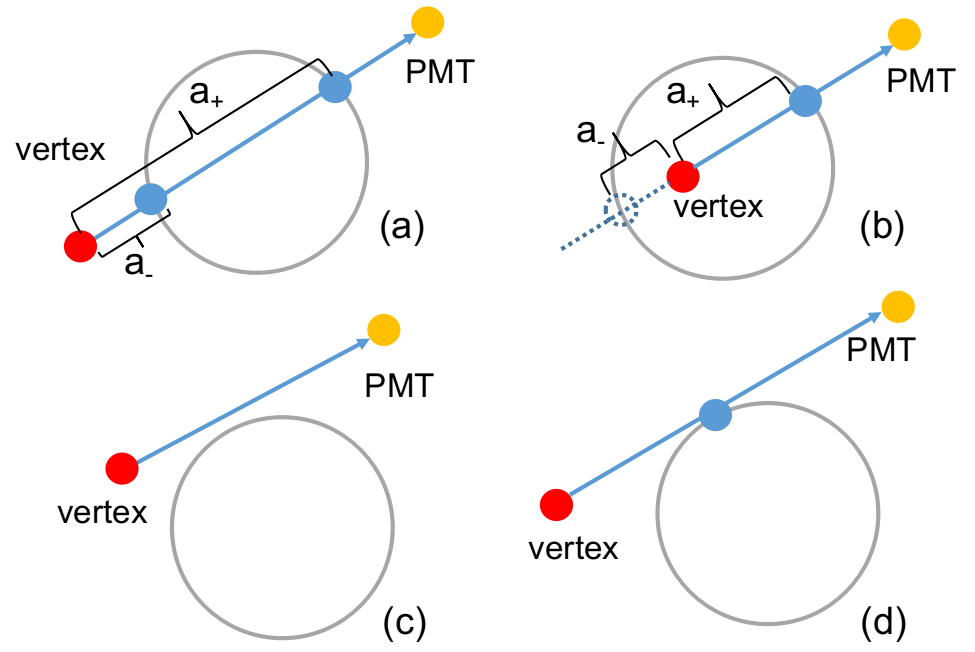
\includegraphics[width=80mm]{line-sphere.png}}
\caption{Line-sphere intersections. (a) the ray vector intersects the sphere with 2 points; (b) the ray vector intersects the sphere with 1 point; (c) and (d): the ray vector never passes through the sphere.}\label{line-sphere}
\end{figure}

\item Ray-plane intersection

For the ray-plane intersection, the z components of the intersection points on $\vec{l}_0$ satisfy the plane equation $z=Z_{split}$, where $Z_{split}$ is the water level, i.e., the z position of the water-scintillator intersection. Thus the intersection equation is:
$l_{0,z}=Z_{split}$, where $l_{0,z}=z_0+a\cdot u_z$.

If $u_z=z_\mathrm{pmt}-z_0=0$, the ray is parallel to the plane and never intersects the plane.

If $u_z\neq 0$, solve the equation, we have: $a=(Z_{split}-z_0)/u_z=(Z_{split}-z_0)$.
Let: 
\begin{equation}
a_3 \equiv a = \frac{(Z_{split}-z_0)|\vec{X}_{\mathrm{pmt}}-\vec{X_0}|}{z_\mathrm{pmt}-z_0}~~(if ~z_\mathrm{pmt}-z_0\neq 0),
\end{equation}

Similar to the case of ray-sphere intersection, if $a_3<0$, the ray-plane intersection point is on the extended line along the opposite direction to the ray; $a_3 \geq 0$ ensures the ray hits the interface. Note that here we consider the plane is infinitely large. Later we will combine with the calculations of the other geometries to cut it off. 

\item Ray-cylinder intersection

For the ray-cylinder intersection, the x and y components of the intersection points on the $\vec l_0$ satisfy the intersection equation: $l^2_{0,x}+l^2_{0,y} = r^2_{neck}$, where $r_{neck}$ is the radius of the neck cylinder ($r_{neck}=785~mm$).

To solve the equation,  let: $\Delta'\equiv [x_0\cdot (x_{PMT}-x_0)+y_0\cdot(y_{PMT}-y_0)]^2 - ( x_0^2+y_0^2-r^2_{neck})\cdot [(x_{PMT}-x_0)^2+(y_{PMT}-y_0)^2]$, and then we get: 
\begin{equation}\label{eq:ray-cylinder}
a'_{\pm} = |\vec{X}_{PMT}-\vec{X}_0|\cdot\frac{-[x_0\cdot (x_{PMT}-x_0)+y_0\cdot(y_{PMT}-y_0)] \pm \sqrt\Delta' }{(x_{PMT}-x_0)^2+(y_{PMT}-y_0)^2},~if~\Delta'>0,
\end{equation}

Similar to the ray-sphere case, if $a'_{+}>a'_->0$, the length of the path inside the cylinder is $a'_+-a'_-$. Due to this geometry, the event position should be outside the cylinder, the condition $(x^2_0+y^2_0)\geq r_{neck}$ is automatically met. If $a'_+>0>a'_-$, the event position should be inside the cylinder and the ray-vector intersects the cylinder with one point (while the other point is along the opposite direction). Thus the length of the path inside the cylinder is $a'_+$. If $\Delta'\leq0$, the ray vector never passes through the neck cylinder. Also note that here we consider the cylinder is infinitely long. This will also be cut off by the combined calculations of the other geometries. In addition, since only the neck region inside the PSUP is valid for the fitter, we should also ensure $z<8390~mm$ (in the PSUP coordination).

\end{itemize}

To evaluate the length of the $|\vec{l}_p|$ in the scintillator region ($d_{sp}$), the above three geometries needs to be combined carefully. The following two procedures go through all the possible situations. First combine the evaluations of the ray-sphere and the ray-plane intersections to calculate the light path in the AV scintillator region ($d_{sp,AV}$). Then combine the evaluations of the ray-sphere and the ray-cylinder intersections to calculate the light path in the neck scintillator region ($d_{sp,neck}$). Detailed algorithms are shown in Appendix.~\ref{appendix:lightpath}.

Since the valid fit requires the events inside the PSUP sphere, only the neck region inside the PSUP sphere (with $6108<z_{neck}<8390~mm$) needs to be considered. The neck path calculation is also allowed to be turned off, while a worse fitted result is expected. Detailed calculations are shown in Appendix.~\ref{appendix:lightpath}.

If $d_{sp}=0$, the light path is always in the water. In this case, the fitter is the same to the \texttt{MP water fitter}. It fits the vertex with the \texttt{MP water fitter} $PDF$. Once the light path passes through the scintillator region, the fitter fits with a scintillator timing $PDF$, in which the PMT time response was modified to photon propagation time in scintillator, as shown in Fig.~\ref{partialpdf}.

\begin{figure}[htbp]
	\centering	
	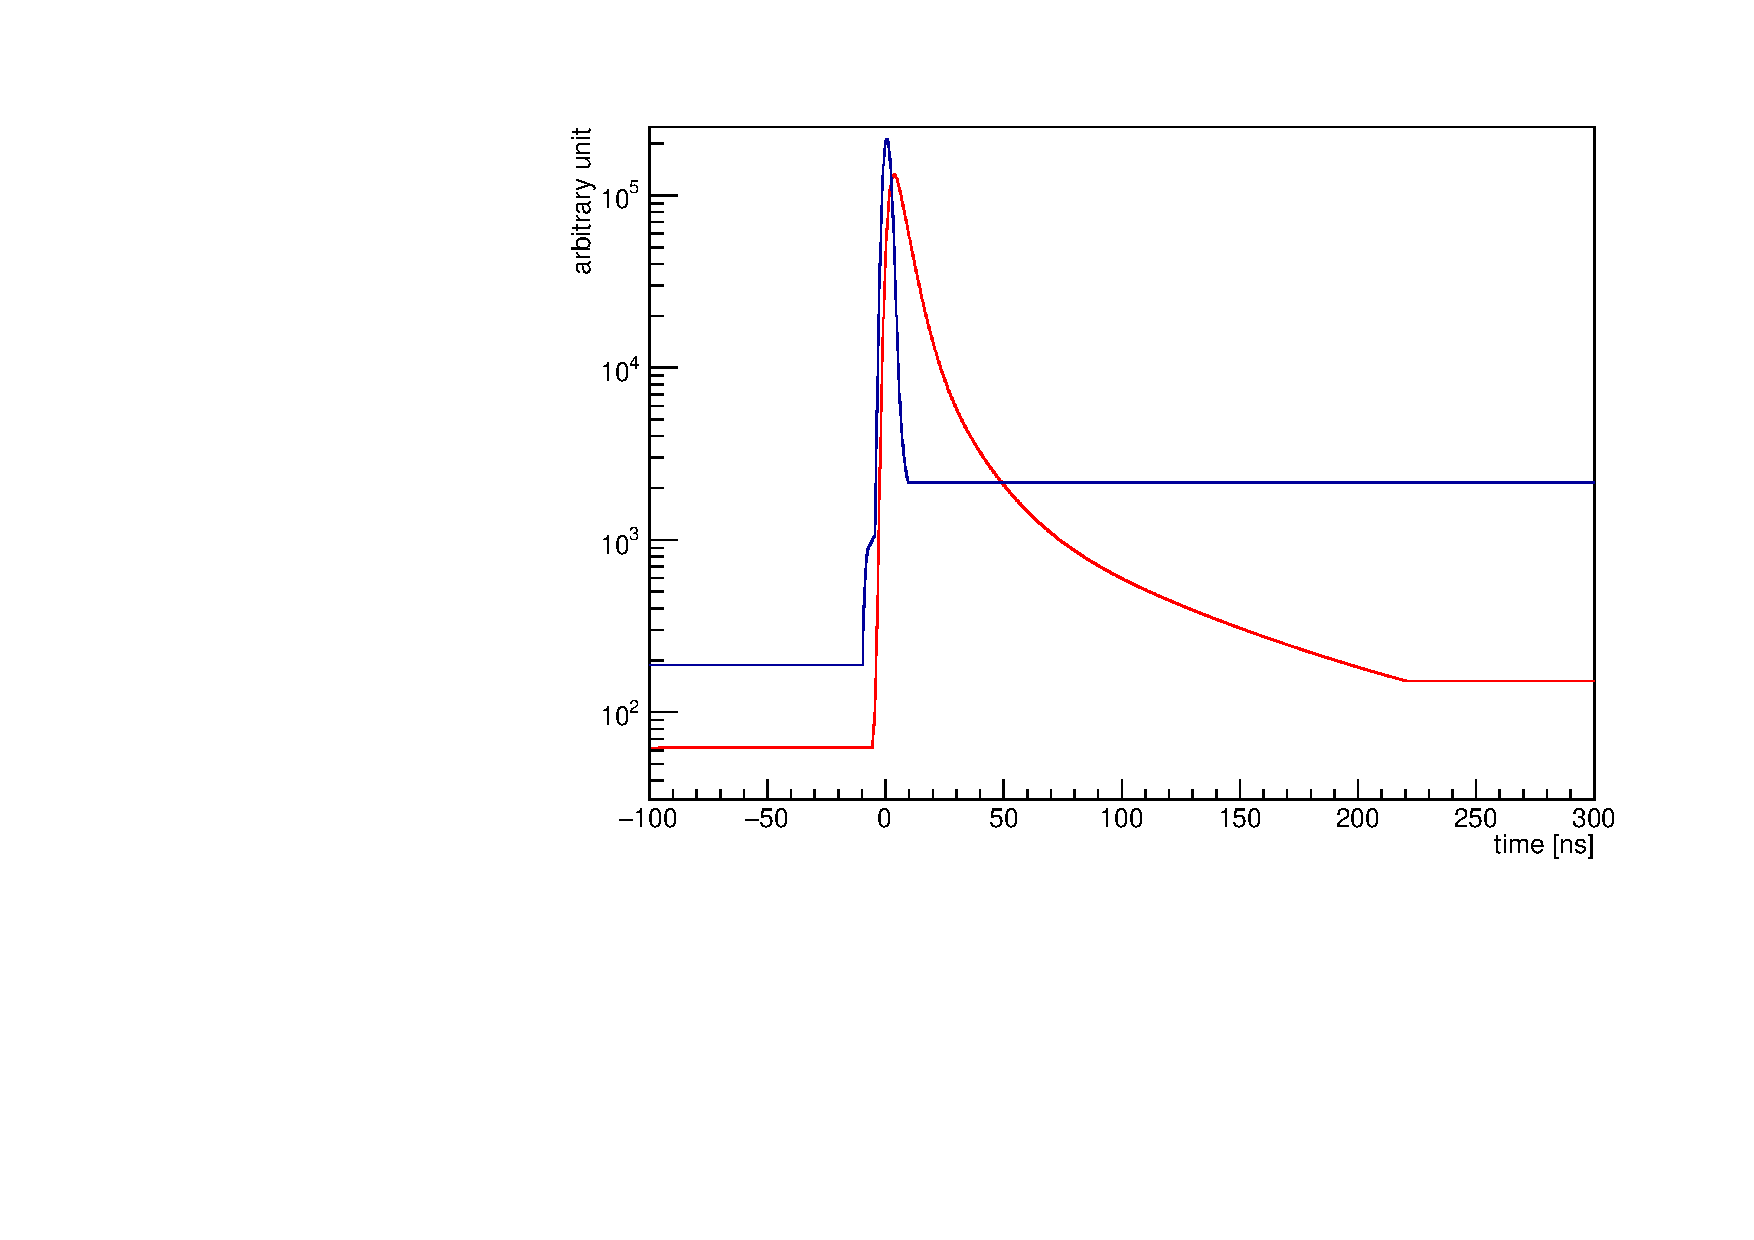
\includegraphics[width=7cm]{scintpdf.pdf}
	\caption{The timing $PDF$s used by the \texttt{MP partial fitter}. Blue: the timing $PDF$ used by the \texttt{MP water fitter}; red: the scintillator timing $PDF$.}
	\label{partialpdf}
\end{figure}

The next section will discuss the timing $PDF$s used by the fitter.

\subsection{Making Timing $PDF$s}

\subsubsection{Different PPO Concentrations during the Filling}
During the partial-fill phase, the water level and the concentration of PPO were changing.

Oxford group in the SNO+ collaboration has done a few bench-top measurements for the time constants and relative light yields of LAB mixed with different concentrations of PPO\cite{oxfordMeasurement}.

The emission time profiles and relative light yields of PPO dissolved in LAB at the following concentrations: 0.25, 0.5, 1.0, 2.0 and 6.0 g/l.

The partial fitter is re-coordinated according to these measurements.

\begin{equation}
\sum_{i=1}^3 (A_i\frac{e^{-\frac{t}{\tau_i}}-e^{-\frac{t}{\tau_{rise}}}}{\tau_i-\tau_{rise}})+A'\frac{e^{-\frac{t}{\tau_{rise}}}}{\tau_{rise}}.
\end{equation}

Based on these measured parameters, $PDF$s were built. 

\begin{table}[ht]
	\centering
	\caption{\label{oxfordMeasure} Time constants and amplitudes measured by Oxford group \cite{oxfordMeasurement}.}	
	{\centering
		\begin{tabular*}{160mm}{c@{\extracolsep{\fill}}ccccccccc}
			\toprule 
			PPO [g/L] & $\tau_{rise}$ [ns] & $\tau_1$ [ns] & $\tau_2$ [ns] & $\tau_3$ [ns] & $A_1$ [\%]  & $A_2$ [\%]   & $A_3$ [\%]  & $A'$ [\%] \\
			\midrule
			0.25 & 1.25 & 8.1 & 25.0 & 68.2 & 29.2 & 53.1 & 13.9 & 3.8\\
			0.5  & 1.12 & 7.2 & 18.7 & 49.1 & 43.5 & 40.4 & 12.6 & 3.5 \\
			1.0 & 1.18 & 5.5 & 13.3 & 40.9 &	45.6 & 37.5 & 13.3 & 3.6 \\
			2.0 & 1.06 & 4.2 & 11.7 & 48.9 & 57.9 & 27.8 & 8.9 & 5.4	\\
			6.0 & 0.94 & 2.5 & 9.3  & 46.0 & 63.7 & 17.0 & 8.6 & 10.7\\
			\bottomrule	
		\end{tabular*}
	}
\end{table}

%\begin{figure}[!htb]
%	\centering
%	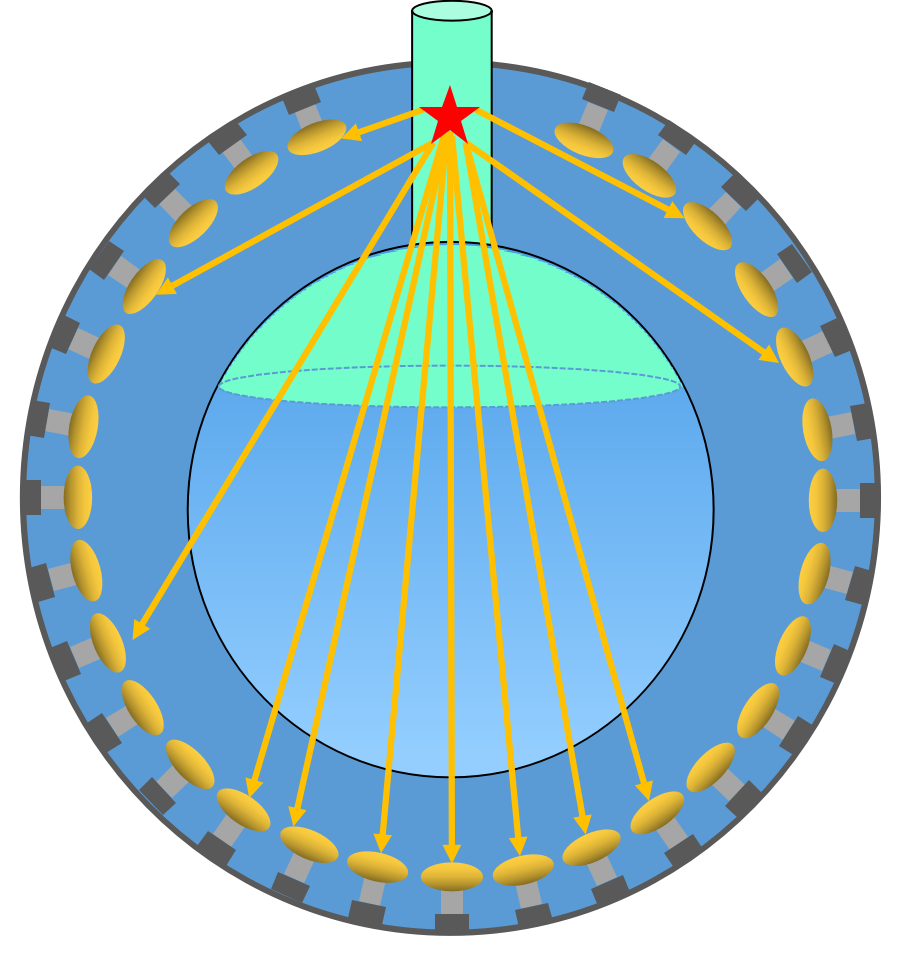
\includegraphics[width=6cm]{skyShine.png}
%	\caption{ Pdfs built for liquid scintillator with various PPO concentrations, based on the bench-top measurements.}
%	\label{oxford_pdf}
%\end{figure}

relative light yield (2 g/L = 11900)
\begin{table}[ht]
	\centering
	\caption{\label{oxfordMeasure2}Relative light yield (RLY) measured by Ref.~\cite{oxfordMeasurement}.}	
	{\centering
		\begin{tabular*}{60mm}{c@{\extracolsep{\fill}}cc}
			\toprule 
			PPO [g/L] & RLY \\
			\midrule
			0.25 & 0.57\\
			0.5 & 0.65\\
			1.0 & 0.9\\
			2.0 & 1.0\\
			6.0 & 0.93\\
			\bottomrule	
		\end{tabular*}
	}
\end{table}

\begin{figure}[!htb]
	\centering
	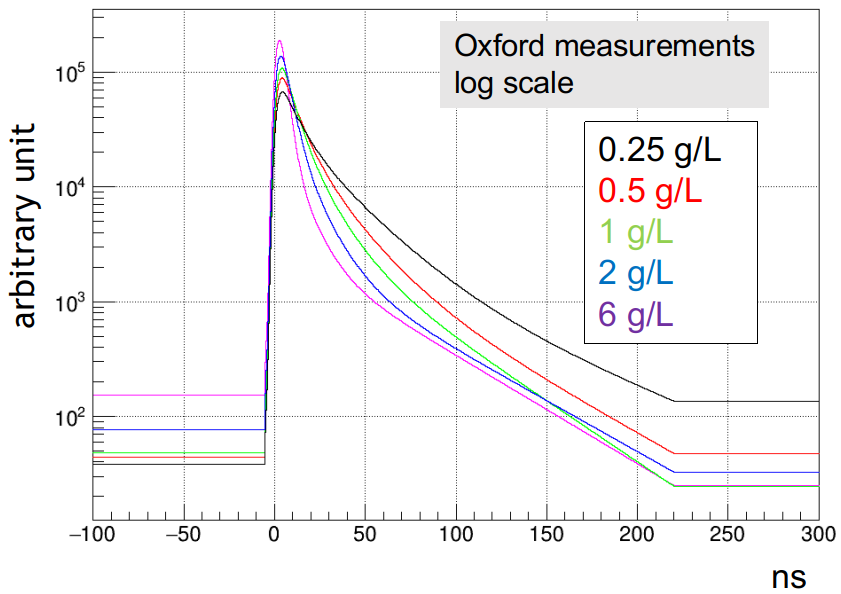
\includegraphics[width=10cm]{oxfordPdf_log.png}
	\caption{Timing spectrum for different PPO concentrations based on the Oxford bench-top measurements.}
	\label{oxfordPdf}
\end{figure}
The partial fitter is invulnerable to the changes caused by different PPO concentrations.

radial biases
\begin{table}[ht]
	\centering
	\caption{\label{partial_groupV}Tuned effective group velocities for different PPO concentrations.}	
	{\centering
		\begin{tabular*}{140mm}{c@{\extracolsep{\fill}}ccccc}
			\toprule 
			PPO [g/L] & $V_{gr,scint}$ [mm/ns]& $n_{scint}$ & $V_{gr,water}$ [mm/ns]& $n_{water,tuned}$\\
			\midrule
			0.25 & 184.068$\pm$5.153 & 1.629 & 211.871$\pm$5.731 & 1.415\\
			0.5  & 183.467$\pm$5.159 &1.634& 211.587$\pm$-5.773 & 1.417 \\
			1.0 & 182.93$\pm$5.193 &1.639& 211.393$\pm$5.805& 1.418 \\
			2.0 & 183.045$\pm$5.184& 1.638& 211.629$\pm$5.767 & 1.417	\\
			6.0 & 184.218$\pm$5.135& 1.627& 211.173$\pm$5.843 &1.420\\
			\bottomrule	
		\end{tabular*}
	}
\end{table}



%& 120.6
%& 90.02
%& 67.39
%& 55.81
%& 58.62

PPO in Fitter configuration
fit with wrong PPO concentrations:  
\begin{table}[ht]
	\centering
	\caption{\label{partial_bias1} Fit position biases for various PPO concentrations.}	
	{\centering
		\begin{tabular*}{140mm}{c@{\extracolsep{\fill}}cccccccc}
			\toprule 
			PPO [g/L] & $\Delta x$ & $\Delta y$ & $\Delta z$  & $\sigma_z$ & $r_{bias}$  & $\sigma_r$ & ratio in FV (\%)&\\
			\midrule
			0.25 & 6.80& 2.90& -14.61& 121.6& -4.82& 120.3& 93.70\%\\
			0.5  & 5.15& 2.82& -12.85 &120.2 &1.34 &123.0 &93.46\% \\
			1.0 &2.32 &1.95 &-13.22& 120.3& 0.344& 121.9 &93.78\% \\
			2.0 &5.76& 3.03& -9.61& 119.3& 7.264 &125.1& 93.26\% \\
			\bottomrule	
		\end{tabular*}
	}
\end{table}

\subsection{Partial Fitter Performances}

The performance of the fitter was studied with MC simulations. In a partial fill geometry with water level at 4.435 m, 2.5 MeV electrons are simulated inside the AV in the scintillator region only, the water region only and the whole AV region.


\begin{figure}[htbp]
	\centering
	\subfigure[scintillator region]{
		\begin{minipage}[t]{0.38\textwidth}
			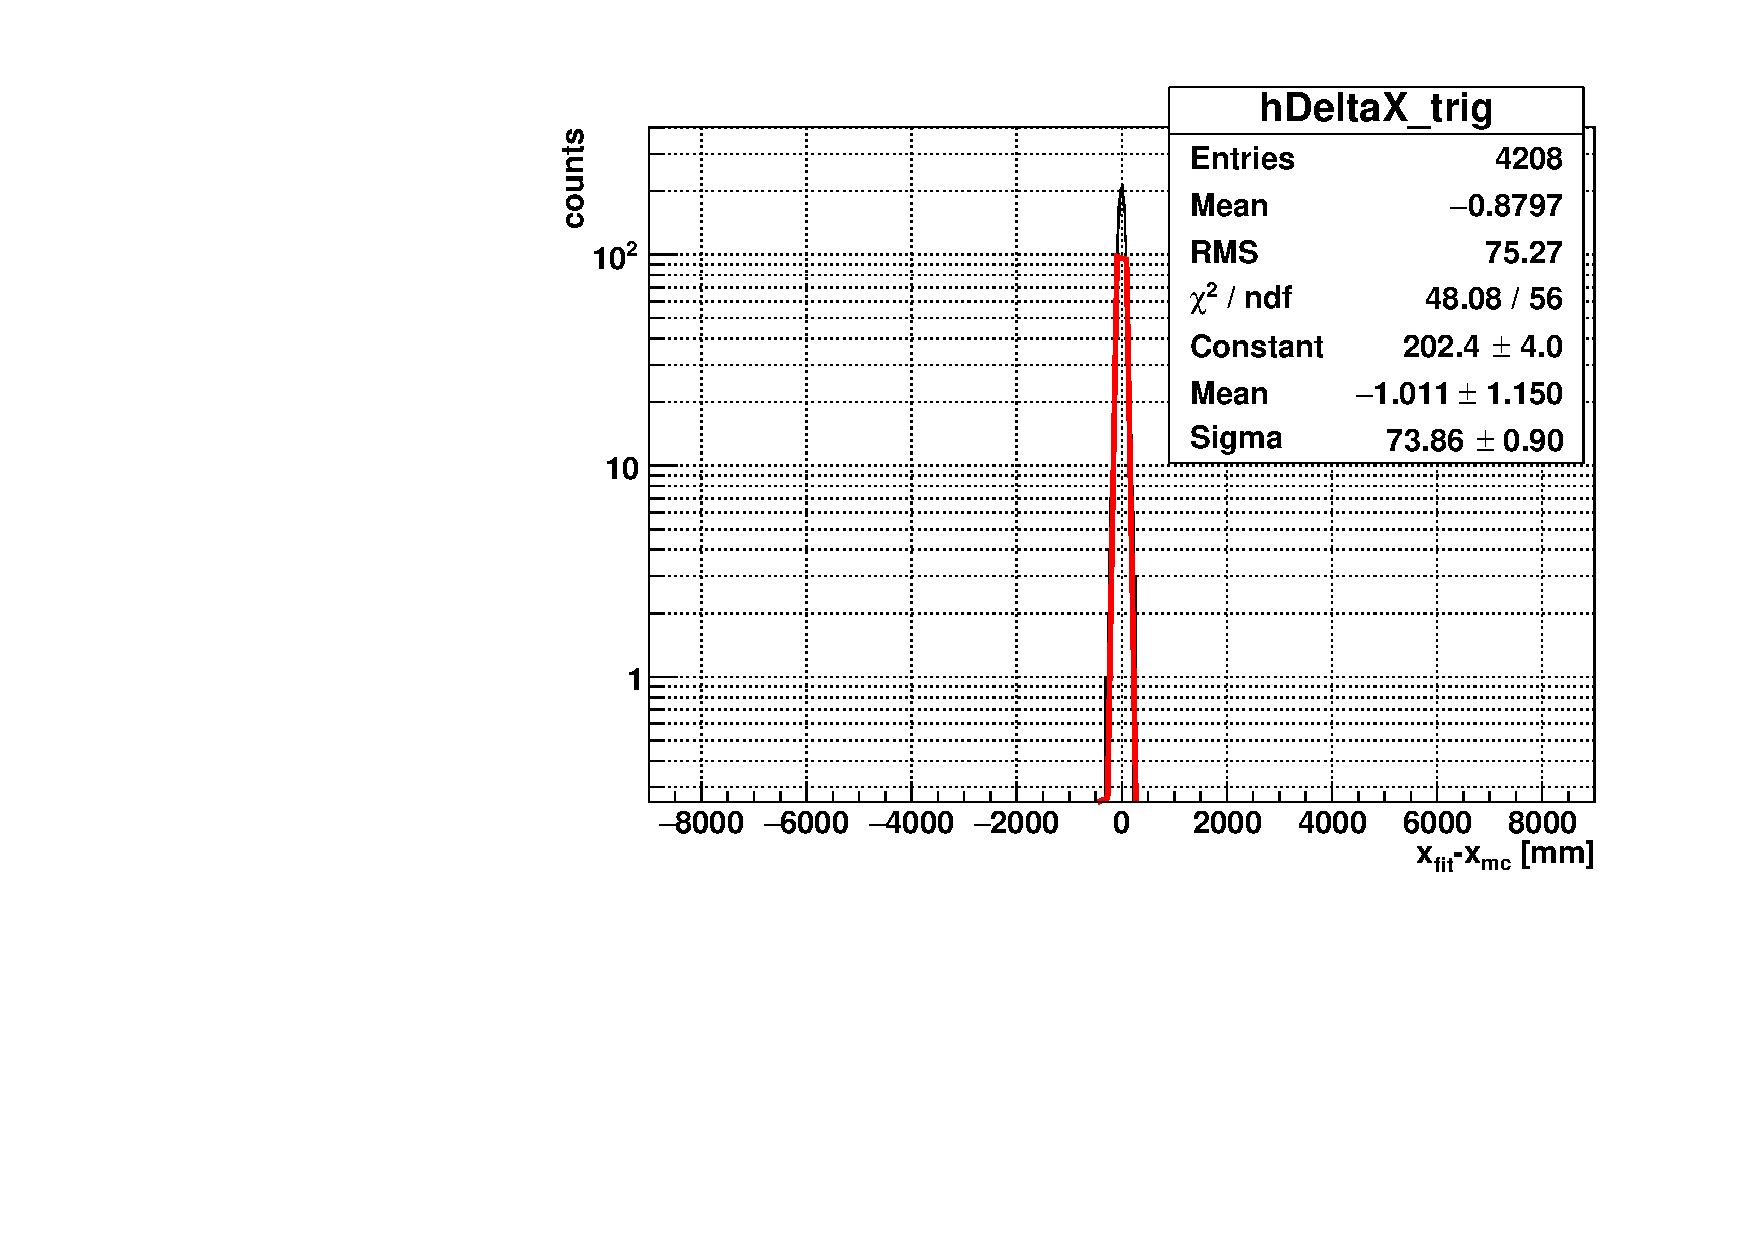
\includegraphics[width=6cm]{partial_top_x.pdf}
		\end{minipage}
	}   
	\subfigure[water region]{ 
		\begin{minipage}[t]{0.38\textwidth}
			\centering
			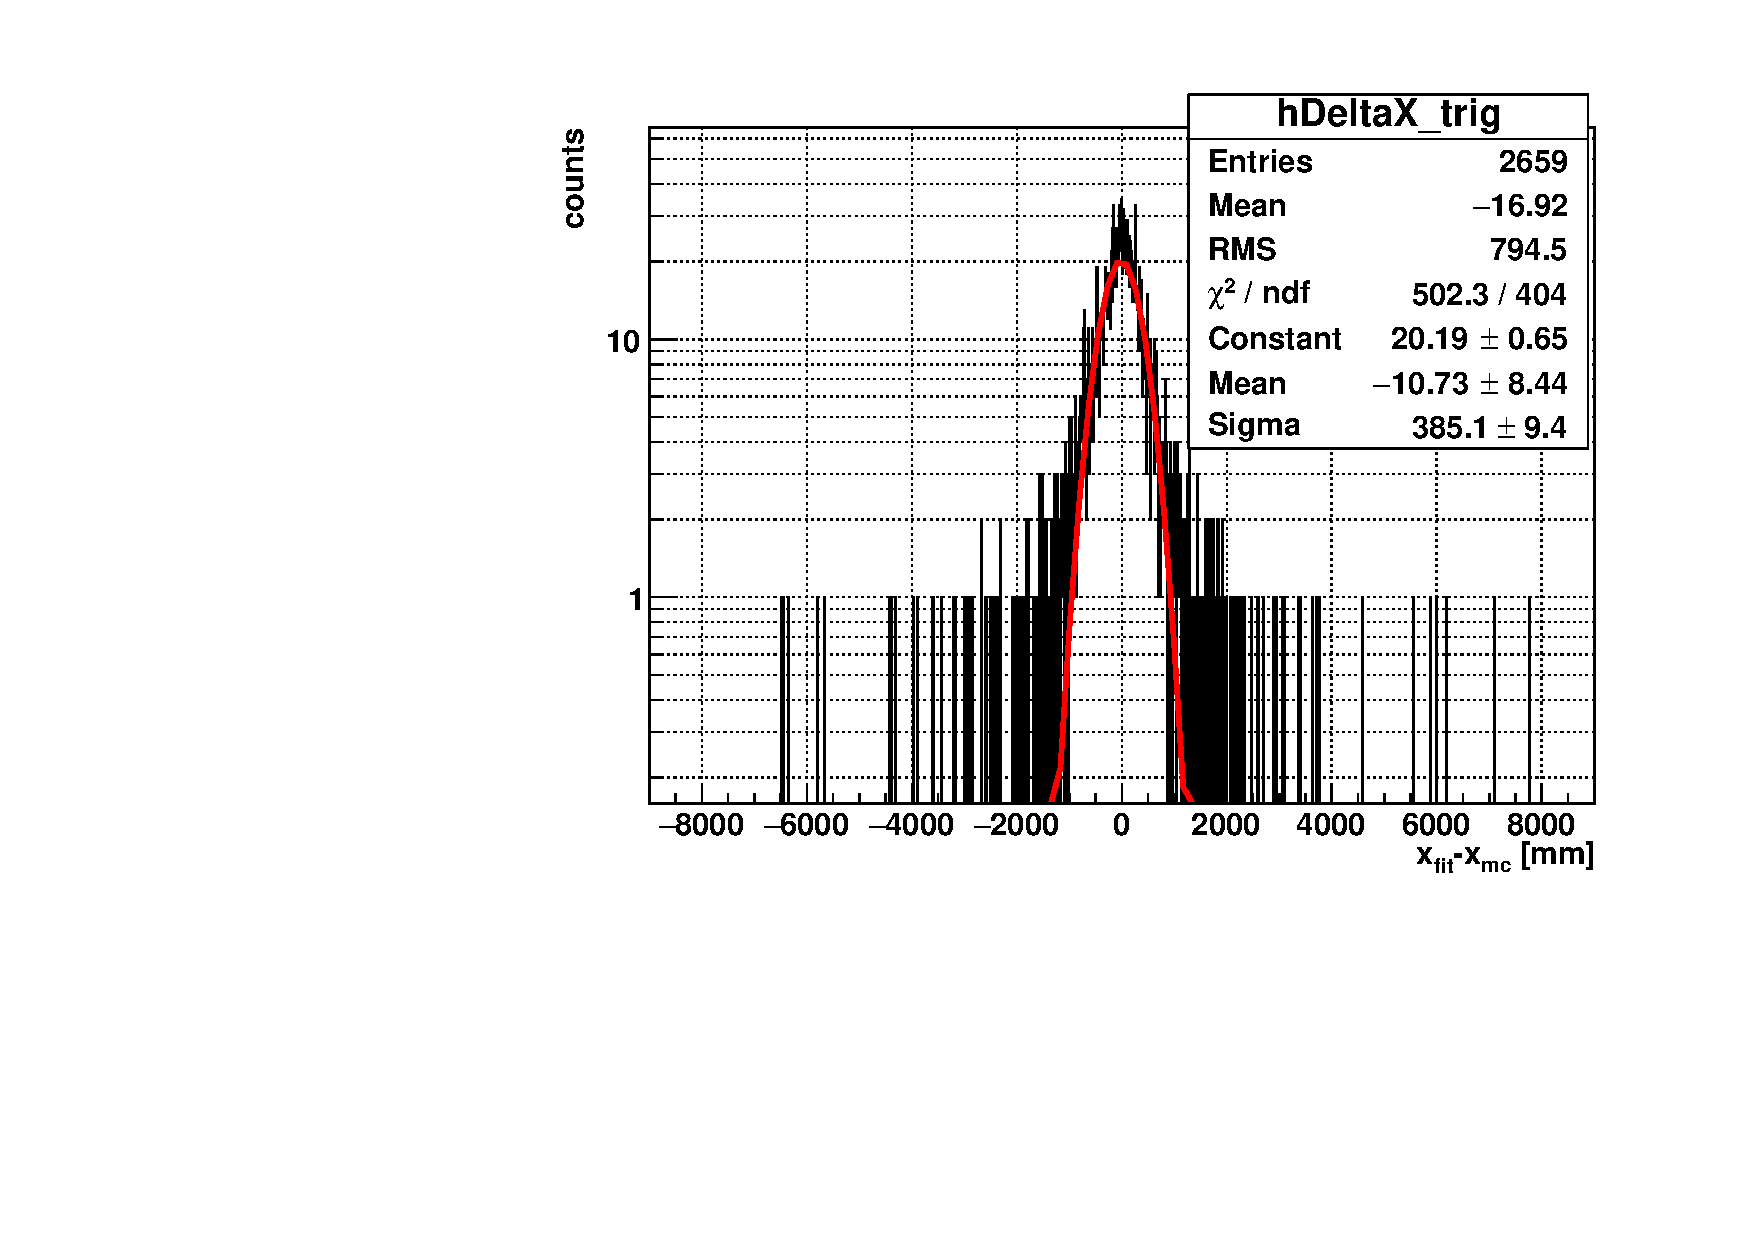
\includegraphics[width=6cm]{partial_bot_x.pdf}
		\end{minipage}
	}
	\subfigure[whole region]{ 
		\begin{minipage}[b]{0.32\textwidth}
			\centering
			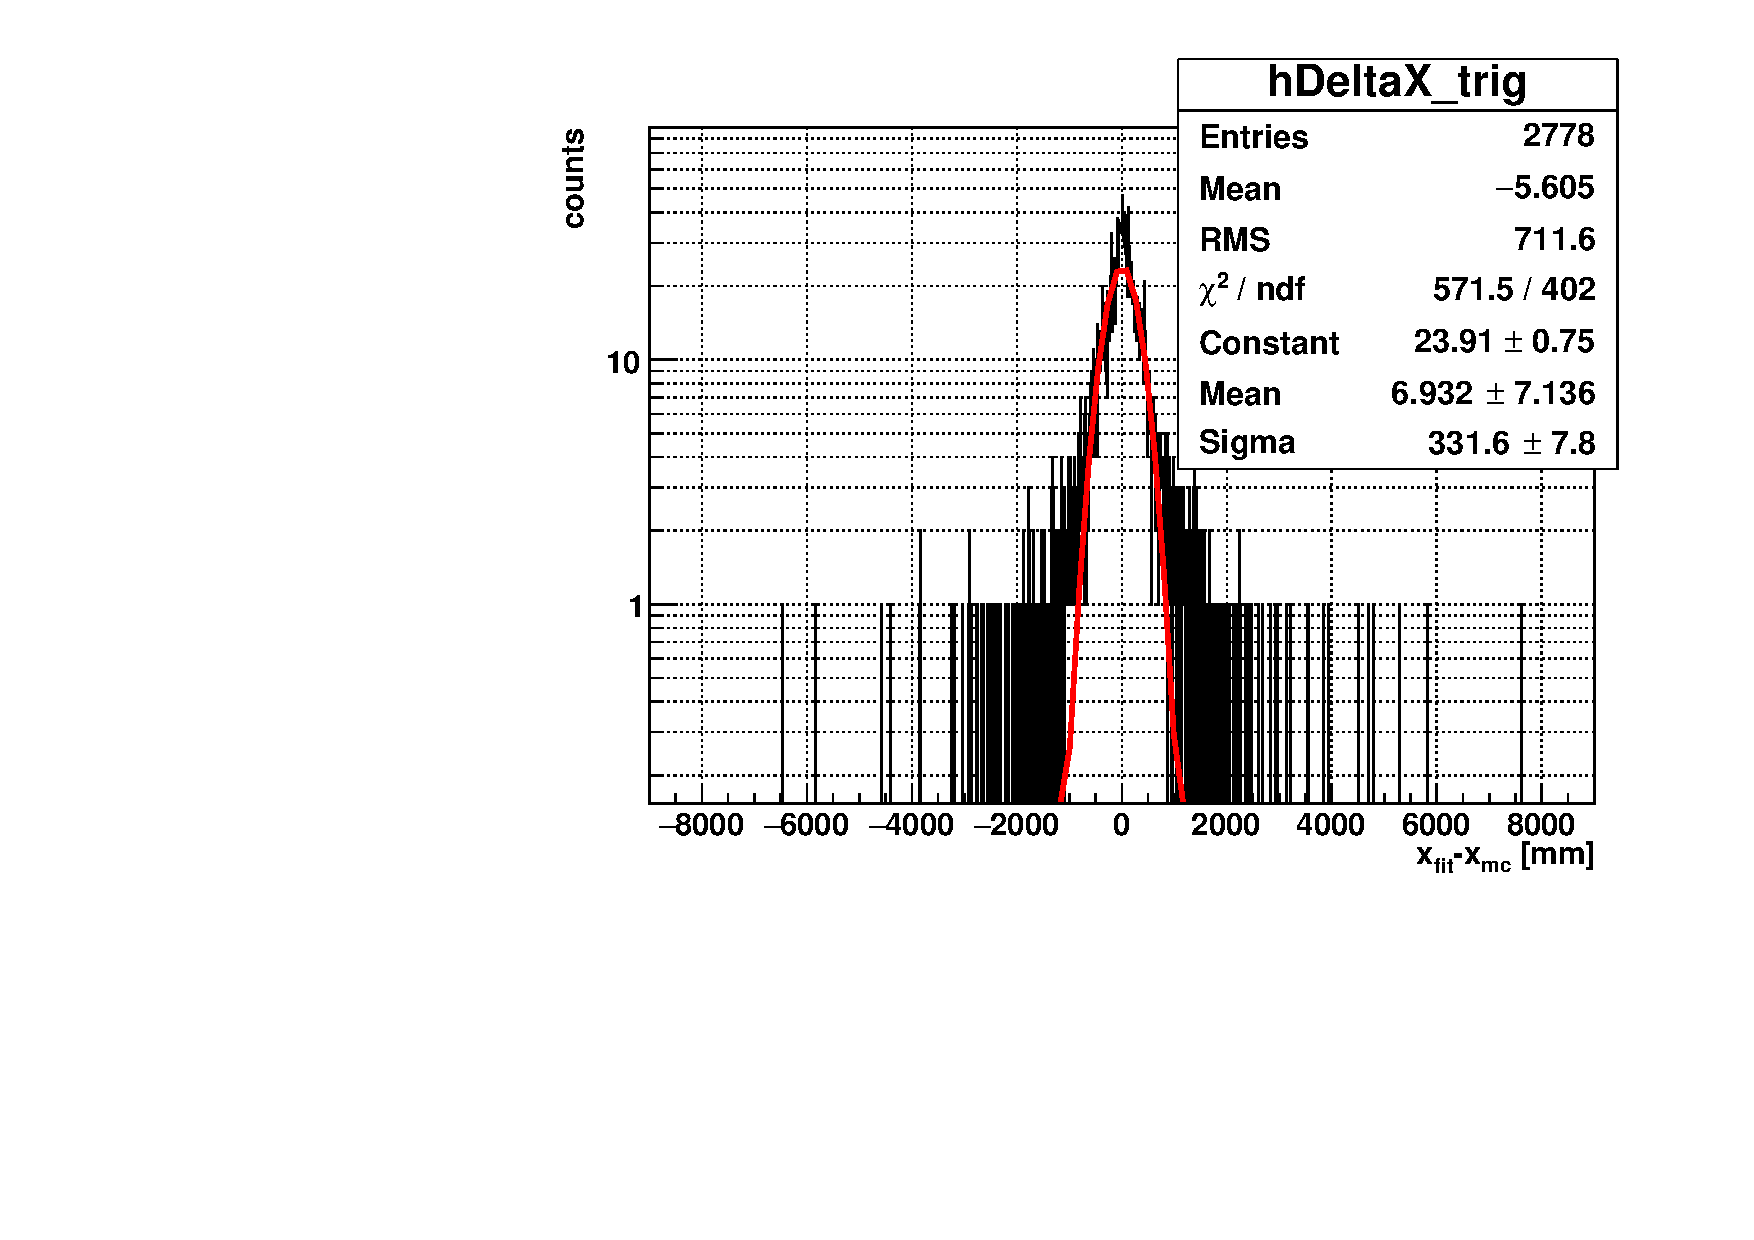
\includegraphics[width=6cm]{partial_full_x.pdf}
		\end{minipage}
	}
	\caption{Distributions of fit position bias projected on x axis ($x_{fit}-x_{MC}$).}
	\label{partial_fit_x}
	\subfigure[scintillator region]{ 
		\begin{minipage}[t]{0.38\textwidth}
			\centering
			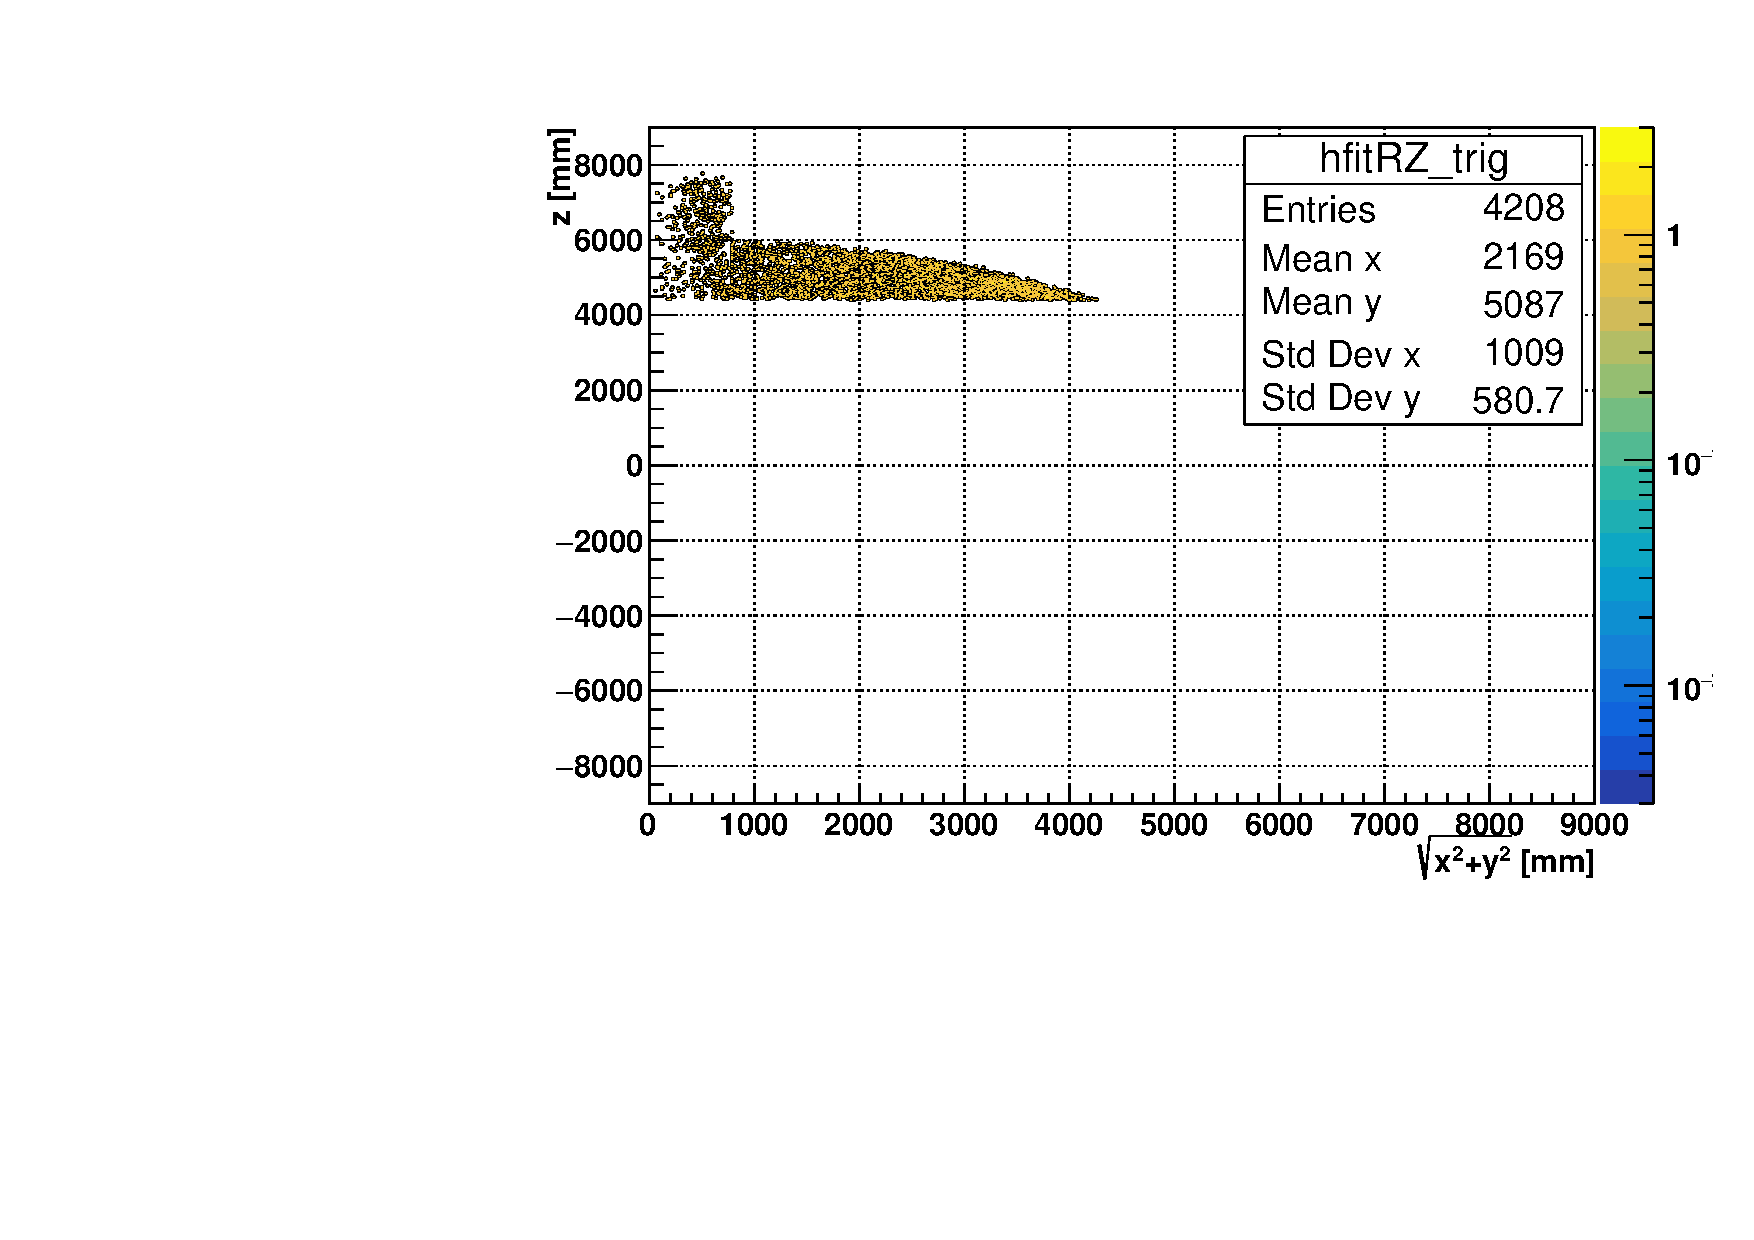
\includegraphics[width=5.8cm]{partial_top_r.pdf}
		\end{minipage}
	}
	\subfigure[water region]{ 
		\begin{minipage}[t]{0.38\textwidth}
			\centering
			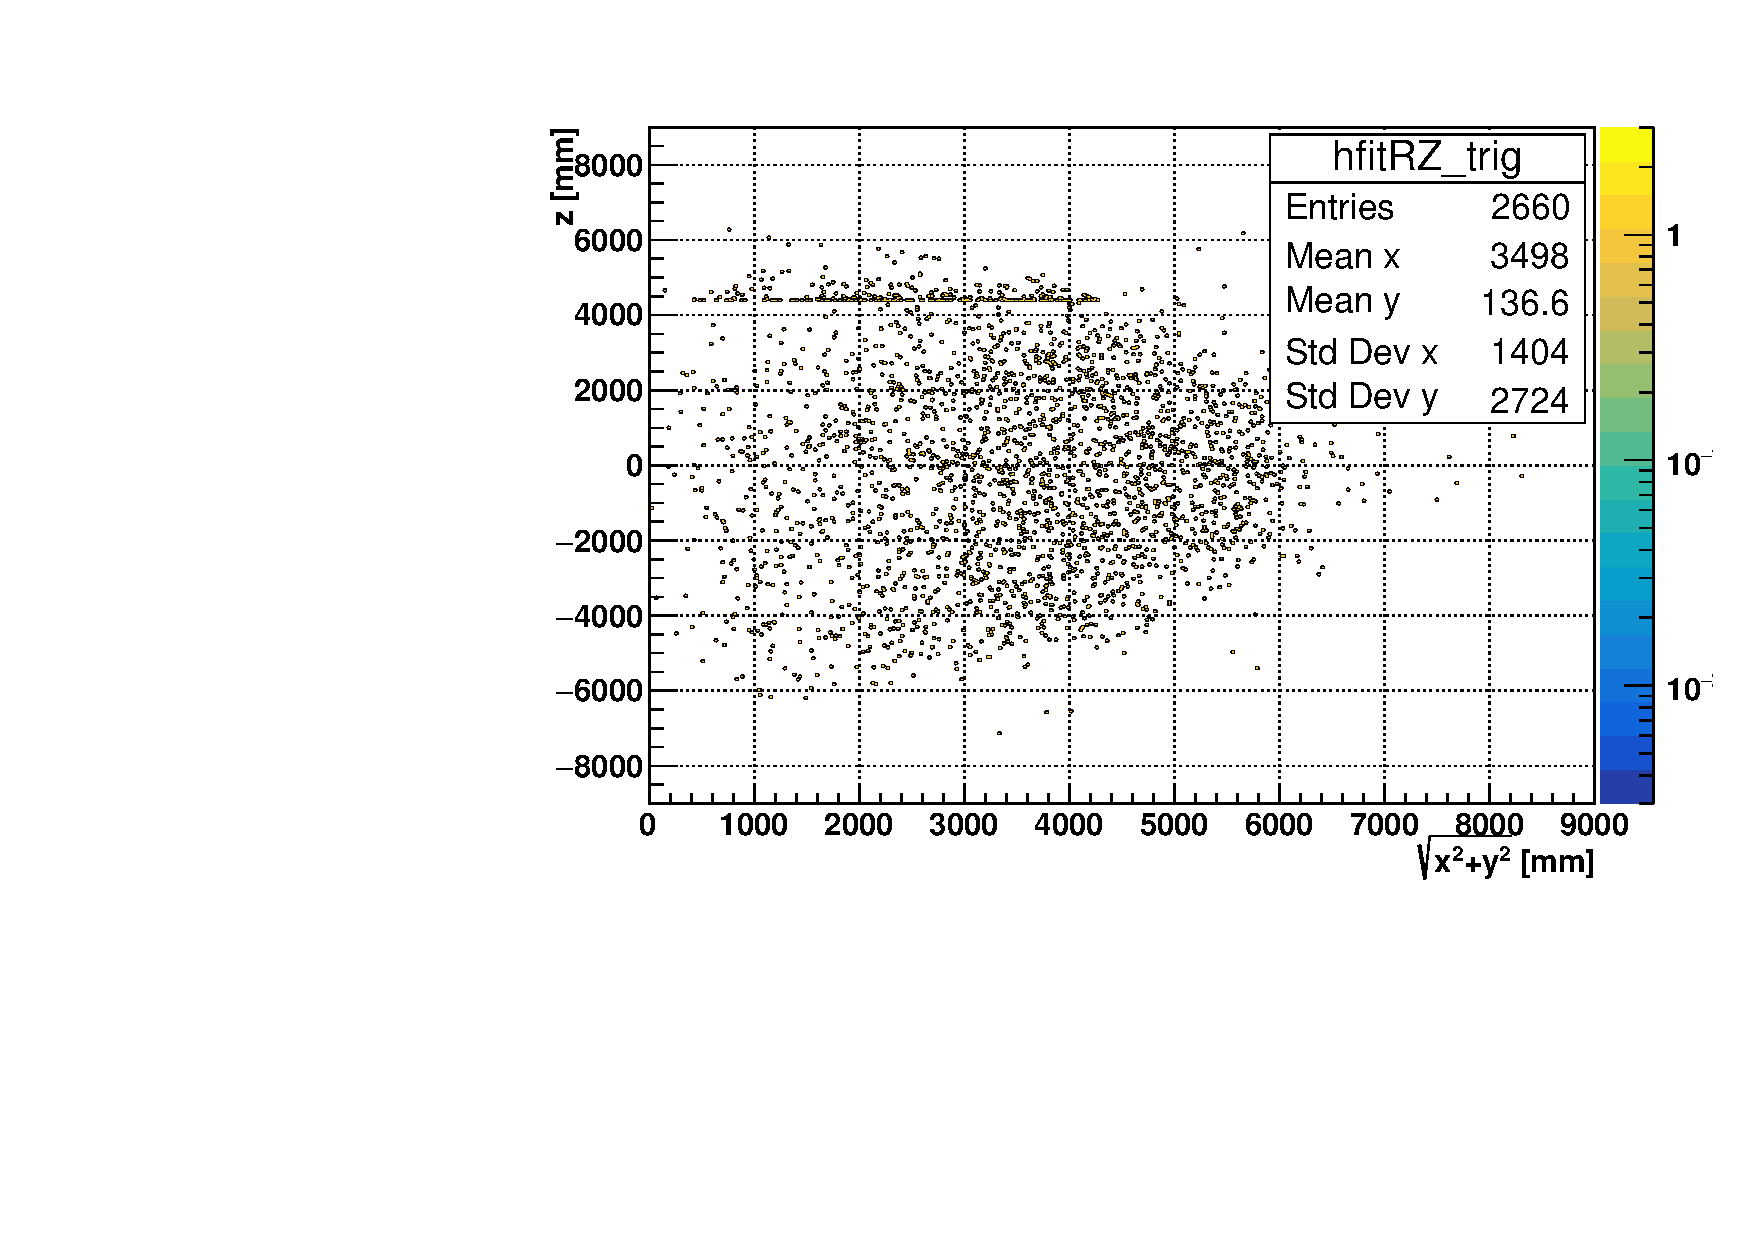
\includegraphics[width=5.8cm]{partial_bot_r.pdf}
		\end{minipage}
	}
	\subfigure[whole region]{ 
		\begin{minipage}[b]{0.35\textwidth}
			\centering
			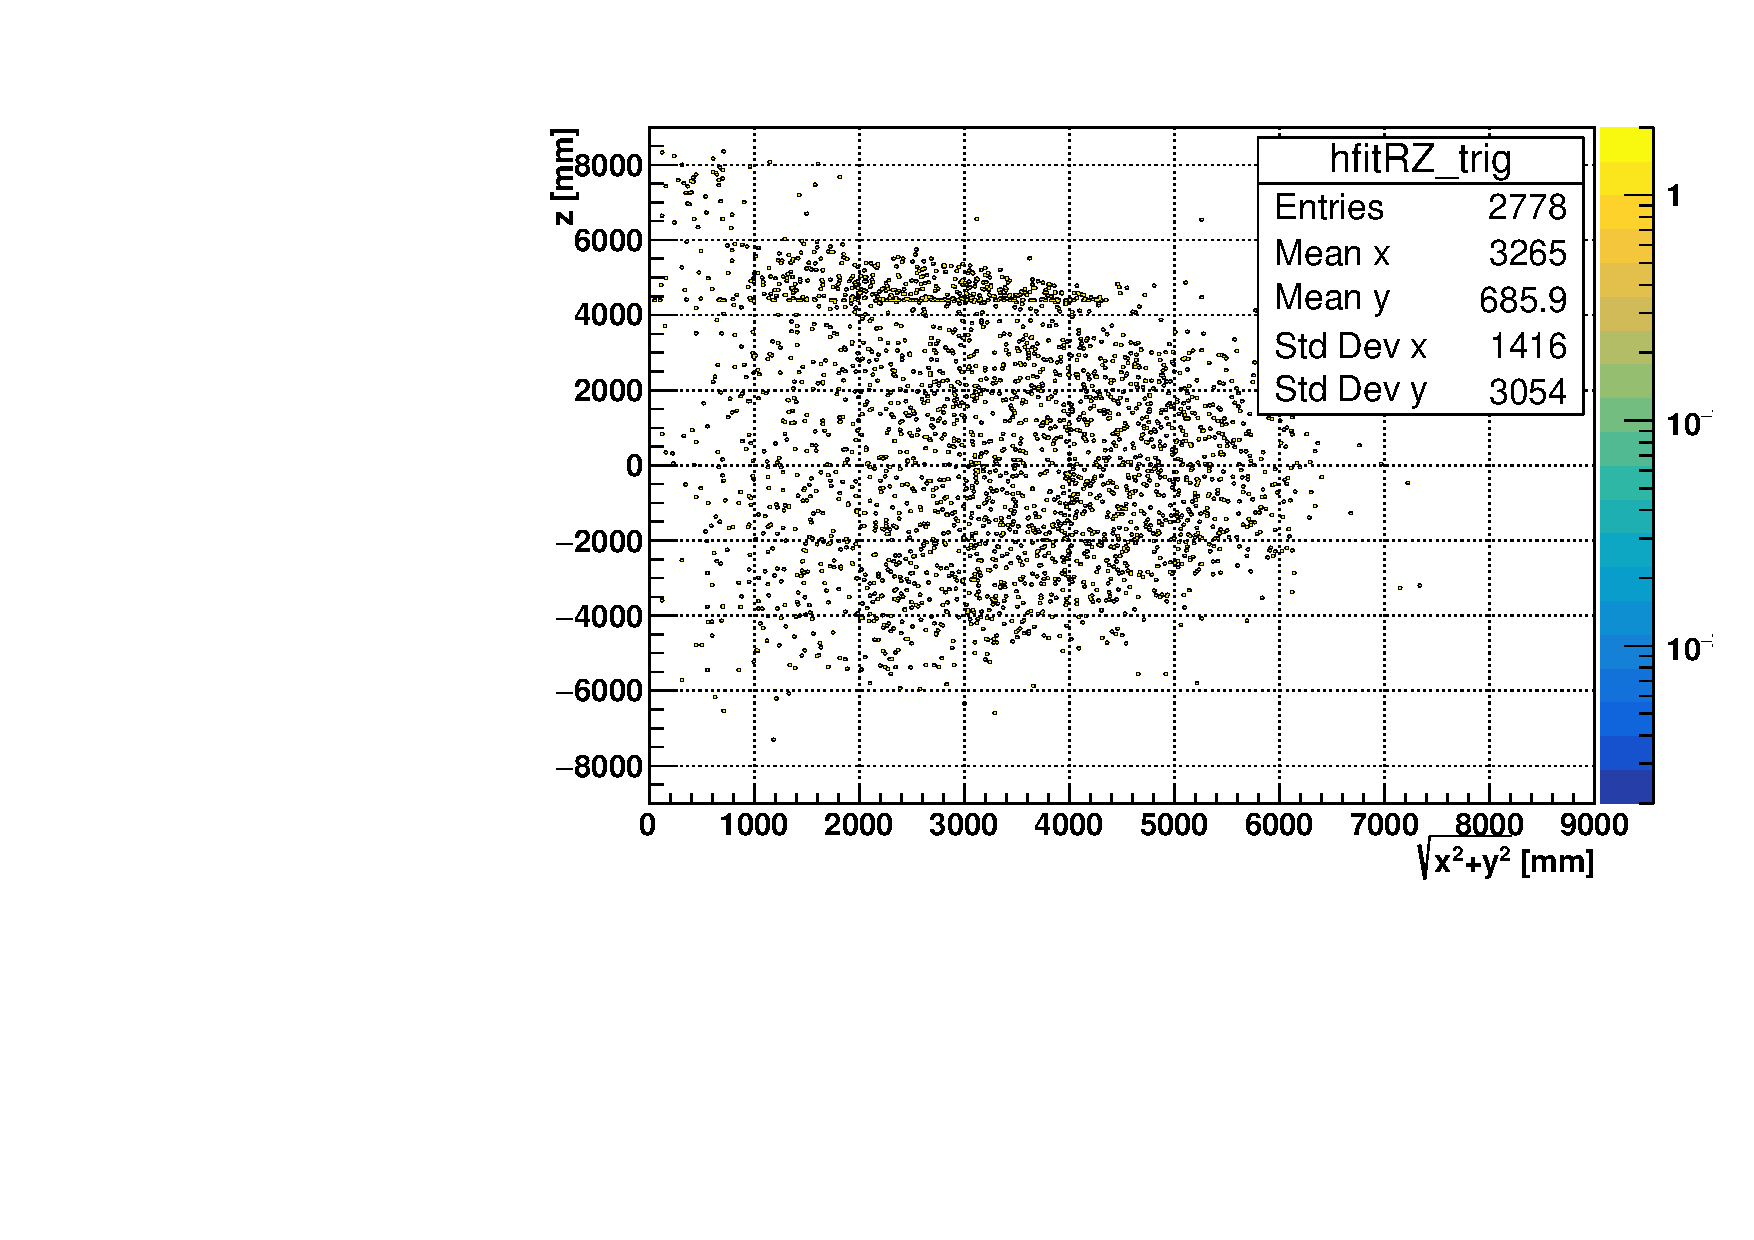
\includegraphics[width=5.8cm]{partial_full_r.pdf}
		\end{minipage}
	}
	\caption{Fit results: $\rho_{fit}=\sqrt{x_{fit}^2+y_{fit}^2}$ vs. $z_{fit}$.}
	\label{partial_fit_rz}
\end{figure}

Fig.~\ref{partial_fit_x} and Fig.~\ref{partial_fit_rz} show the MP Partial Fitter reconstructed results for these simulations. Fig.~\ref{partial_fit_x} shows the biases between the fit positions and MC positions, projected on the x axis. The distributions of position biases are fit with Gaussian functions. The values of Gaussian mean and sigma quantify the fit biases and resolutions. Table~\ref{partiaResol} lists these values.

\begin{table}[ht]
	\caption{Reconstructed position biases and resolutions for simulated events in partial fill.}
	\label{partiaResol}
	\centering
	\begin{tabular*}{120mm}{c@{\extracolsep{\fill}}ccc}
		\toprule
		regions of simulated events& bias (mm) &  resolution (mm) \\
		\hline
		scintillator region & -1.0  & 73.9\\
		water region & -10.7 & 385.1\\
		full region &6.9 & 331.72\\
		\bottomrule
	\end{tabular*}
\end{table}
For the events in water, the fit bias and resolution is comparable to the water phase results in Table~\ref{table_posresol}. The events in the scintillator region have smaller fit bias and better resolution due to more hit PMTs in the reconstruction.

Fig.~\ref{partial_fit_rz} shows the fitted $\sqrt{x^2+y^2}$ vs. fitted $z$ positions. It shows that the fitter can distinguish different events in the water or scintillator region. The fitter gives reasonable results of the three different MC simulations. 

$PDF$s for all timing \ref{sect:LS_SNO+}.


Radial bias is defined as the difference between the fitted and true position, projected along the radial component (unit vector) of the true position \cite{coulter2013modelling}.
\[
(\vec{X}_{fit}-\vec{X}_{true})\cdot \hat{X}_{true}
\]

The value of the mean radial bias is taken by fitting the histogram of the distributions of radial biases with a Gaussian profile and then get the mean of the fitted Gaussian profile.


\subsubsection{Test on Different PPO Concentrations}
Simulate 5000 events for 3-MeV $e^-$,  $\Delta x = x_{fit}-x_{mc}$

\begin{table}[ht]
	\centering
	\caption{\label{partial_bias} Fit speeds and biases for various PPO concentrations.}	
	{\centering
		\begin{tabular*}{145         mm}{c@{\extracolsep{\fill}}cccccc}
			\toprule 
			PPO [g/L] & fit speed [s/event]& $\Delta x$ [mm]& $\Delta y$ [mm]& $\Delta z$ [mm] & $r_{bias}$ [mm] & \\
			\midrule
			0.25 & 0.190 &6.65 &2.64& -18.24& -7.22\\
			0.5  & 0.144 &-0.73 &-1.69& -8.14& 3.30 \\
			1.0 &0.190 & 1.42 &0.57 &-5.65& 10.67 \\
			2.0 &0.194 & 0.34 &1.78& -4.01& 13.37	\\
			6.0 &0.145 & -0.11& -0.12& -25.97& -10.97\\
			\bottomrule	
		\end{tabular*}
	}
\end{table}

%% fit resolutions
$z_{fit}$ resolution [mm] 

\subsection{Test on Background Simulations}

\subsection{Bi-Po Simulations}
The Bi-Po analysis was performed on simulations to check the fitter efficiency. This analysis suggests a model offset of the water level to include more fitted data. A flowchart of the algorithm for picking up the Bi-Po event pairs is shown in Appendix.~\ref{appendix:bipo}, Fig.~\ref{biPo_flowchart}.



\subsection{Discussions for the Partial Fitter}
An attempt to use the \texttt{MP partial fitter} to fit the water level was discussed \cite{mpFitWaterLevel}.
\[
\frac{\partial L}{\partial splitZ} = \frac{\partial L}{\partial tof}\cdot\frac{\partial tof}{\partial splitZ}=\frac{\partial L}{\partial tof}\cdot\frac{\partial a_3}{\partial splitZ}
\]

\[
\frac{\partial L}{\partial splitZ} = 0
\]

%Appendix: Levenberg-Marquardt method for fitter minimization
(ref: press2007numerical)

The fit results gave a Gaussian resolution of $293.9$ mm, which is much larger than the position resolution and is not good enough for the analysis.

%for M unknown parameters: $a_0, a_1, ... , a_{M-1}$ (for example, the 4 parameters of an event vertex: $(x,y,z,t)$)

The $PDF$ can be expanded and fit with Chebyshev polynomials to obtain an analytic approximation function\cite{press2007numerical}. This analytical function can give proper analytical derivatives.


\section{Vertex Reconstruction for the Scintillator Phase}\label{sect:scintFitter}
As mentioned in the last section, the vertex reconstruction for the scintillator phase is similar to the partial-fill case, while no water-scintillator interface is considered here since the AV is fully filled with liquid scintillator. Only the ray-sphere and ray-cylinder intersections are calculated and thus the major code of the \texttt{MP scint fitter} was modified directly from the \texttt{MP partial fitter} by removing the ray-plane intersection calculations.

\subsection{Performance of the Vertex Reconstruction}

Since the 2.5-MeV event is the major interested signal in the scintillator and tellurium-loading phases, 10000 2.5-MeV $e^-$ events were simulated at random positions inside the AV and with isotropic directions. 

Fig.~ shows the performance of the \texttt{MP scint fitter} for this set of simulations. The histograms of the fit position biases were fitted with Gaussians. A position resolution of 
%%fullScint_2p5MeV_rhoVsZ.png

For other energies, the Gaussian means and resolutions were shown in .

It is ob
down to the 1 MeV, with a position resolution of 91 mm.

\begin{figure}[htbp]
	\centering
	\subfigure[$x_{fit}-x_{mc}$]{
		\begin{minipage}[t]{0.38\textwidth}
			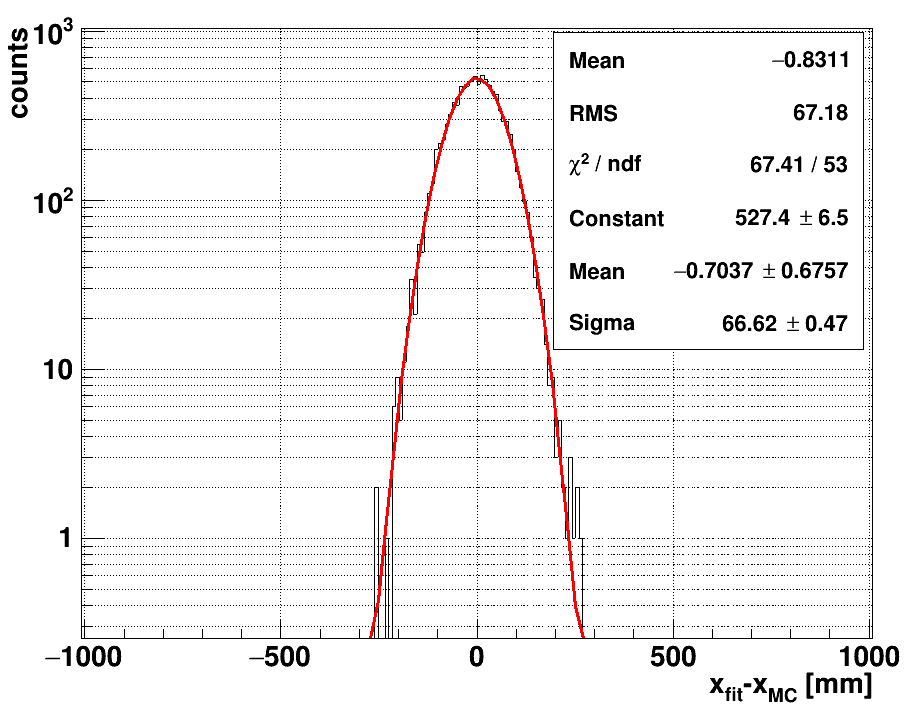
\includegraphics[width=6cm]{fullScint_2p5_xbias.png}
		\end{minipage}
	}   
	\subfigure[$y_{fit}-y_{mc}$]{ 
		\begin{minipage}[t]{0.38\textwidth}
			\centering
			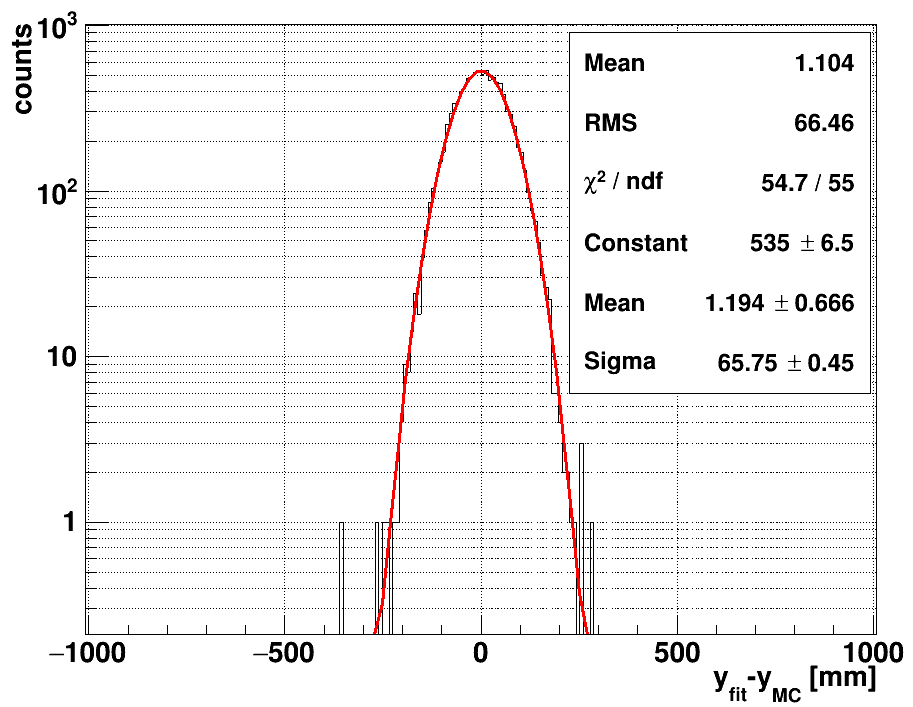
\includegraphics[width=6cm]{fullScint_2p5_ybias.png}
		\end{minipage}
	}
	\subfigure[$z_{fit}-z_{mc}$]{ 
		\begin{minipage}[b]{0.38\textwidth}
			\centering
			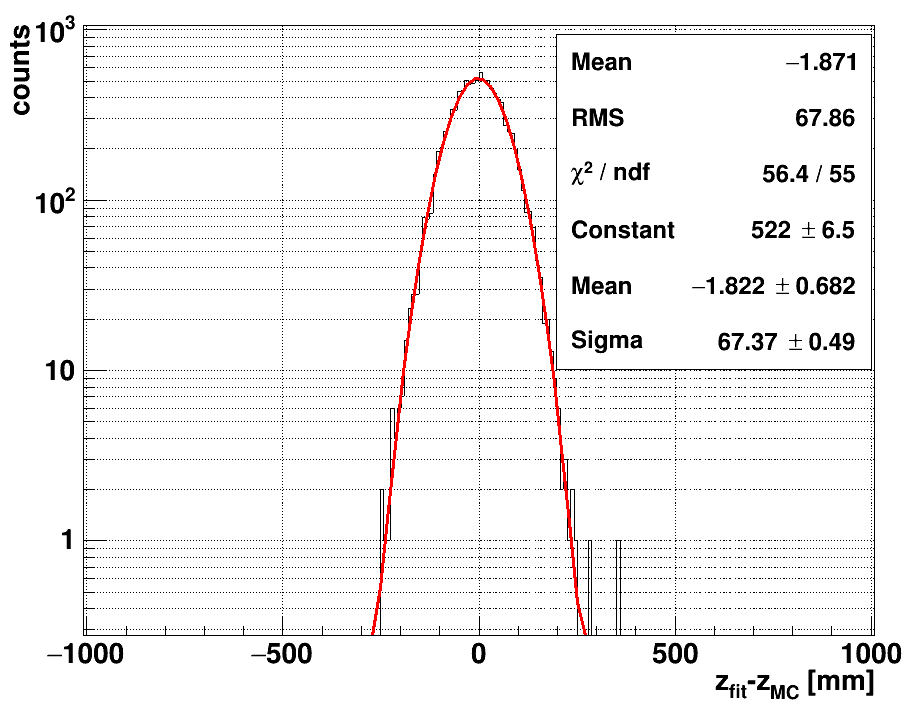
\includegraphics[width=6cm]{fullScint_2p5_zbias.png}
		\end{minipage}
	}
	\subfigure[$(\vec{X}_{fit}-\vec{X}_{mc})\cdot \hat{X}_{mc}$]{ 
	\begin{minipage}[b]{0.38\textwidth}
		\centering
		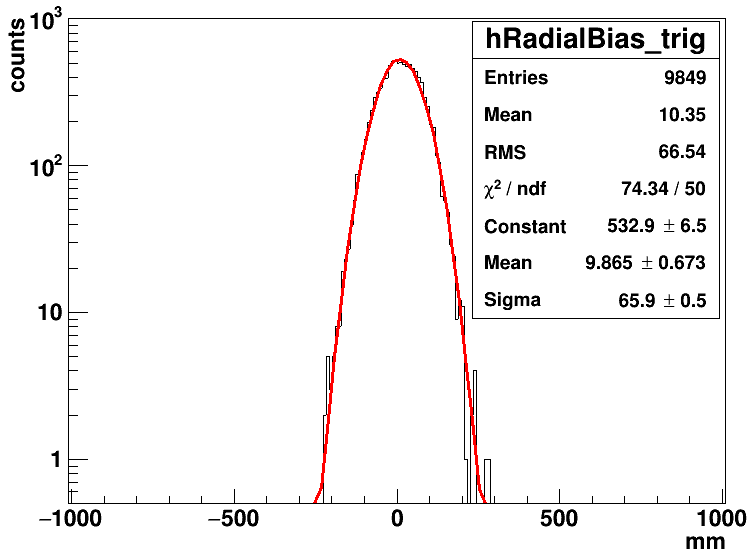
\includegraphics[width=6cm]{fullscint_2p5MeV_radialBias.png}
	\end{minipage}
    }
	\caption{Distributions of fit position biases for 10000 MC simulations of 2.5-MeV $e^-$ events.}
\end{figure}


\section{Multi-path Fitter Structure for Multiple SNO+ Physics Phases}

The \texttt{MP fitter} has already been implemented into the \texttt{RAT} software for data processing and analyzing. Following the \texttt{RAT} event reconstruction structure, the \texttt{MP fitter} is feasible to tackle with multiple SNO+ physics phases. 

The \texttt{MP fitter} first loads the fitter data base. The database contains the parameters used by the fitter, including the physics constants (e.g., speed of light), detector geometry parameters (e.g., $r_{PSUP}$, length of neck, water level), fitter setting parameters (e.g., the effective group velocity, fitter iteration number, etc.) and $PDF$s. It is included in the \texttt{RAT} database (ratdb) in a \texttt{JSON} format\cite{JSONwiki} and contains tables which are tagged by different indices to indicate specific physics phases or detection medium. For example, for the partial-fill phase with a PPO concentration of 0.5 g/L, the fitter extracts the $PDF$s and fitter setting parameters under the index of ``labppo\_0p5\_scintillator''. These fitter setting parameters and $PDF$s were optimized for the 0.5 g/L PPO partial-fill geometry.

Then the \texttt{MP fitter} goes through the event-by-event reconstruction. For a triggered event, it calls PMT selectors and sends the information of the selected PMTs to a \texttt{Likelihood Calculation Class}. Section \ref{sect:PMTselector} will give the details about the PMT selectors. In the \texttt{Likelihood Calculation Class}, there are mainly 4 likelihood calculation functions\footnote{The \texttt{AirWaterVertex} for the early partial water fill test in 2014 and the \texttt{WavelengthShifterVertex} for the conceptual wavelength-shifter test, as mentioned in the previous sections, were not included in the current version of \texttt{RAT} since they are not used in actual physics phases.}: the \texttt{WaterVertex} and \texttt{WaterDirection} for the event vertex and direction reconstruction in the water phase; the \texttt{ScintWaterVertex} for the vertex reconstruction in the partial-fill phase; and the \texttt{ScintVertex} for the vertex reconstruction in scintillator and tellurium-loading phases.

Reading the detector geometry settings as well as the assigned index of detection medium, the fitter selects proper likelihood functions to construct the likelihood functions and to calculate the likelihoods and their derivatives by evaluating fit parameters based on different light path calculations in different detector geometries. The calculated likelihoods and derivatives are sent to the MRQ method class to maximize the likelihood and finds the best-fit values. The MRQ method class does not care about how the likelihood functions are constructed and how the likelihoods and derivatives are calculated. 
	
A \texttt{Dump Likelihood Class} stores the trial fit parameters with respect to their likelihoods and derivatives for interested events by designating their event GTIDs in the database. By looking at the likelihood surfaces and derivatives of the interested event, the fit performance of that event can be checked to see whether the fitter finds the global or local maximum. Sect.~\ref{appendix:likelihoodSurface} shows an example of the dumped likelihood surfaces and derivatives for an $^{16}$N event vertex reconstruction. 

Once the reconstructed results are obtained, the fitter will send them to the classifiers for further analysis calculations. 

\section{PMT Selectors for the Reconstruction}\label{sect:PMTselector}
Several PMT selectors are used to select or remove PMTs from all the recorded PMTs triggered by an event and send the proper PMTs to the fitter for reconstruction. They are developed for optimizing the fitter or boosting up the fit speed:

\begin{itemize}
	\item[$\bullet$] Straight Light Path Time Residual Cut Selector
	
	This selector is used for the direction reconstruction for the SNO+ water phase. It is first developed by Singh for the MultiPath fitter. In the selector, the value of time resifal ($t_{res}$) is calculated for each hit PMTs from an event and the PMT with a $t_{res}$ value in a prompt time window of $[-10.0, 120.0]~ns$ is selected for the fitter. The selector calculates $t_{res}$ by using straight line light path, which is the same to the MultiPath water fitter. This can remove the PMTs triggered by photons with late timing, such as the photons reflected off the detector elements (late light) and keep the possible Cherenkov ring hit pattern clear for the direction fitter to fit. Also, dropping the irrelevant PMTs can potentially boost up the fit speed.
	
	\item[$\bullet$] Mode Cut Selector
	
	This selector was developed by the collaboration for all fitters. It checks the hit time ($t_\mathrm{PMT}$) distributions of all the hit PMTs and finds a mode value of the hit time ($t_{mode}$). If $t_{mode}$ fails to be found, it calculates a median value ($t_{median}$) instead\cite{modeCut}. Then it selects the PMT with $t_\mathrm{PMT} \in [t_{mode}+t_{low}, t_{mode}+t_{high}]~ns$. This selector is used to remove the PMTs triggered by noise and light light from reflection. The values of $t_{low},~t_{high}$ are optimized for different scintillators. For the MPW fitter, the optimized window is $[t_{mode}-50, t_{mode}+100]$ ns by checking with the fit biases and resolutions for the \isotope[16]{N} central run data in the water phase, while for the MP scint-water fitter the optimized window is $[t_{mode}-100, t_{mode}+100]$ ns based on checking with the simulations.
	
	\item[$\bullet$] Uniform PMT Selector
	
	I designed this selector for the partial-fill phase and the scintillator phase when a single event can trigger a large amount of PMTs. It reduces the number of the hit PMTs to a designated number ($n_{select}$) in order to boost up the fit speed. When an event triggers $N$ calibrated PMTs, the selector goes through these recorded PMTs and uniformly picks up one PMT by an interval of $\left \lceil{N/n_{select}}\right \rceil $. If $N\leq n_{select}$, the selector does nothing. By doing this, the selector uniformly reduces the number of the PMTs for the fitter without an obvious bias.
	
	\item[$\bullet$] Earliest Hit PMT Selector
	
	Similar to the uniform PMT selector, this selector reduces the number of the hit PMTs to boost up the fit speed. It first groups the PMTs by their positions in the PMT support sphere. Take the centre of the sphere as coordinate origin, the sphere is divided by the azimuth angle $\phi$ (as longitude) and zenith angle $\theta$ (as latitude). In the sphere, the positions of the PMTs in $\phi$, ranging in $[-\pi,\pi]$, is uniformly divided into $n$ intervals while the positions of the PMTs in $\cos\theta$, ranging in $[-1, 1]$, is also divided into $n$ intervals. Thus, the PMTs are grouped into $n\times n$ panels, see Fig.~\ref{GroupPMTs}. 
	\begin{figure}[!htb]
		\centering
		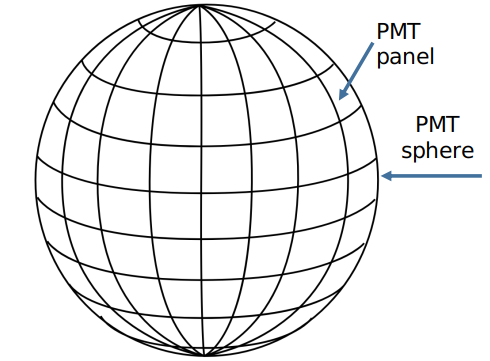
\includegraphics[width=5cm]{GroupPMTs.png}
		\caption{Group the PMTs by dividing the PMT sphere with latitudes and longitudes.}
		\label{GroupPMTs}
	\end{figure}
	
	For each panel, the selector first drops the PMTs triggered too early ($t_\mathrm{PMT}<100~ns$, where $100~ns$ is set as a default threshold). These PMTs could be triggered by noises, such as pre-pulsing. In the rest of the PMTs, the selector picks up one PMT with the earliest $t_\mathrm{PMT}$ in each panel. Thus the number of the PMTs is reduced to $n\times n$ for the fitter, i.e., $n_{select}=n\times n$. If $N\leq n_{select}$, the selector does nothing. 
	
	The other timing parameters can also be used for selecting the PMT in each panel, such as the $t_{mode}$ or the $t_{median}$. However, tests from the simulations for the scintillator phase show that using the earliest hit time gives less fit biases and better fit resolutions.
\end{itemize}

\section{Energy Reconstruction}
The SNO+ energy fitter mainly uses a lookup table to convert number of hit PMTs (NHits) and position in the detector into a reconstructed energy.

For the energy reconstruction in the water phase,  

energy response processor, or the energy RSP fitter, is derived from SNO \cite{boulay2004direct,moffat2001optical}.

It uses the fitted position and direction of an event as inputs and then calculates an effective 

estimated $N_\gamma$,

detailed detector effects are taken into account.

the asymmetric geometry of the detector, for example the neck cylinder on the top of the AV sphere; the actual number of online PMTs in a realistic physics run.

\isotope[16]{N} calibration scans at certain detector points.

Energy lookup table built from the simulation data set.

energy look up\cite{energyRSP}.
(\texttt{energyRSP})

%     A lookup table is used to
%	// map from estimated Cerenkov photons to energy. 
%	
%	the PMT efficiency, and the position and angular dependence of the $NHits$ is also taken into account. 
%	
%	// This method calculates the optical response of each PMT (taking into
%	// account PMT efficiency, solid angle, Cerenkov angular distribution,
%	// etc.) to estimate the number
%	// of Cerenkov photons from the prompt hits. This fitter is only
%	// for a detector geometry with light water in the inner av.


\subsection{Figure of Merit}\label{sect:energy_fom}
Three figure of merit quantities for the energy fitter were developed by the SNO+ collaboration in order to identify the poor reconstructed results which have large biases to the true energy values, especially for the low energy regions around 2.2 MeV, which helps the analysis of neutron capture\cite{waterunidoc}.

%Water Reconstruction Errors & FOMs 6190
\begin{itemize}
	
	\item[$\bullet$]$U$-test ($U_{test}$):
	A Mann-Whitney quantity uses the channel hit probabilities by EneryRSP which are ordered and ranked. The rank of the channels with hits are summed.%cite logan docDB 6190	
		\begin{equation}
		U_{test}\equiv \frac{S-N(N+1)/2}{N(N_{active}-N)},
		\end{equation}
	where $S\equiv \sum_{i}^N \mathrm{rank}_i$. 
	
	\item[$\bullet$] $G$-test ($G_{test}$):
	A quantity uses the hit probabilities by EnergyRSP ($E_i$) which are normalized to the number of observed hits ($N$) %cite logan docDB 6190	
	
	\begin{equation}
	G_{test}\equiv \frac{1}{N}\sum_{i=1}^N \log(\frac{1}{E_i}),
	\end{equation}
	
	\item[$\bullet$] $Z$-factor ($Z_{factor}$):
	A quantity uses the medians and median absolute deviations
of hit probabilities by EnergyRSP
	
	\begin{equation}
     Z'\equiv 1-\frac{3(\sigma_p+\sigma_n)}{\mu_p-\mu_n},
    \end{equation}
\end{itemize}

\subsection{Energy Reconstruction in Partial-fill Phase}
Up till this thesis writing, there is no proper energy fitter for the partial-fill phase works. I attempted two methods for the energy reconstruction in the partial-fill phase: the NHit scale method and the NHit ratio method. Both of them are based on the simulations. These two methods need more effects to be improved.
\subsubsection{NHit Scale}
In the partial-fill phase ,  In \cite{partialEnergy}, 
to scale $\mathrm{NHits}$ based on several sets of simulations.

\subsubsection{NHit Ratio}

The fitter follows the idea of the charge-ratio fitter for the partial energy reconstruction\cite{partialEnergyYang}.

\begin{equation}
E = p_0+p_1\cdot NHit+p_2\cdot NHit^2
\end{equation}


$\mathrm{NHits}$ ratio table based on position.


\section{Other Reconstruction Algorithms}
\subsection{Hough Transformation for Direction Reconstruction}

Hough transformation is a pattern recognition algorithm used in image analysis and computer vision\cite{davies1997machine}. This algorithm was first invent to extract patterns in bubble chamber\cite{houghwiki}, 

is used by Super-K\cite{shiozawa1999reconstruction}.

The Hough transformation algorithm was used in SNO data analysis for counting the numbers of the Cherenkov rings caused by multiple charged particles in a high energy event such as atmospheric neutrinos event\cite{bonventre2014neutron}. It is also suggested for the reconstruction of event direction in the SNO+ scintillator phase\cite{houghTransform}.

As illustrated in Fig.~\ref{houghTrans}, 

circular Hough transformation
\begin{figure}[!htb]
	\centering
	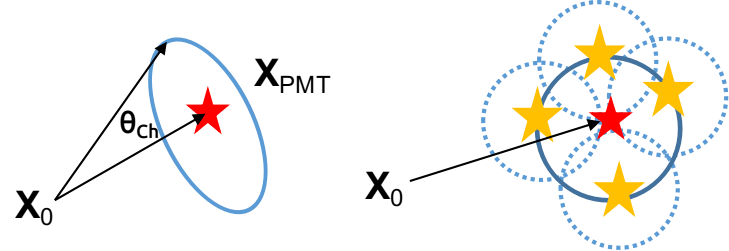
\includegraphics[width=8cm]{houghTransform.png}
	\caption{Hough transformation for catching the ring structure of Cherenkov signals and fitting the direction.}
	\label{houghTrans}
\end{figure}

\subsection{Deep Learning}
Nowadays, the vast amount of data available to particle experiments make it feasible to implement machine learning and deep learning methods for data analysis. At the time of this writing, a deep learning framework is being developed\cite{markMachineLearning,markNeuralTalk,markNeuralNetwork}. This method investigates the relation between the hit PMT distributions and the event reconstruction, currently for the position and direction. It trains neural networks based on the MC simulation datasets (with $\mathcal{O}(10^6)$ events) as well as the calibration datasets to predict the event position and direction\cite{markNeuralTalk}. A few physics-based loss functions, such as the loss function checking the $t_{res}$, can be further included to improve the reconstruction performance\cite{markNeuralTalk}. 

Once the neural networks are trained, the reconstruction speed is expected to be 100 to 1000 times quicker than the traditional likelihood-fit method if running on the CPU (Central Processing Unit), and since the deep learning method can also utilize the computing power of the GPU (Graphics Processing Unit), it is expected to be 10000 times quicker\cite{markNeuralTalk,markNeuralNetwork}. Such a fast speed reconstruction will be promising to be applied in the scintillator phase where it is time-consuming for reconstructing the higher $\mathrm{NHits}$ events. The deep learning framework is also expected to aid the data analysis.

\section{Conclusion}
The Multi-path Fitter framework of event vertex reconstruction was developed for multiple SNO+ physics phases. Under this framework, the \texttt{Multi-path Water Fitter} works as an alternative fitter to provide additional reconstruction information for the water data and it gives proper position and direction resolutions for the water analysis. The \texttt{Multi-path Scint-Water Fitter} works as the prime fitter for the SNO+ partial-fill phase.